\documentclass[whitelogo]{TUD-report2020}

\usepackage[style=apa]{biblatex}
\addbibresource{report.bib}

\usepackage{changes}
\usepackage{graphicx}
\usepackage{amsmath}
\usepackage{hyperref}

\widowpenalties 1 10000
\raggedbottom
\setcounter{tocdepth}{1}

\begin{document}

%% Use Roman numerals for the page numbers of the title pages and table of
%% contents.
\frontmatter

%% Uncomment following 19 lines for a cover with a picture on the lower half only
\title[tudelft-white]{Identification of Near-Earth Asteroids using Multi-Spacecraft Systems}
\author[tudelft-white]{J. G. P. Vermeulen}
\affiliation{Technische Universiteit Delft}
\coverimage{img/cover.png}
%\titleoffsetx{10cm}
\titleoffsety{10cm}
%\afiloffsetx{1cm}
\afiloffsety{18cm}
\covertext[tudelft-white]{
    \textbf{Master Thesis}}
\makecover

%% Uncomment following 16 lines for a cover with a picture on the lower half only
%\title[tudelft-white]{Identification of Near-Earth Asteroids using Multi-Spacecraft Systems}
%\author[tudelft-white]{J. G. P. Vermeulen}
%\affiliation{Technische Universiteit Delft}
%\coverimage{img/cover.png}
%\covertext[tudelft-white]{
%}
%\setpagecolor{tudelft-cyan}
%\makecover[split]


%% Include an optional title page.
\begin{titlepage}


\begin{center}

%% Insert the TU Delft logo at the bottom of the page.

%% Print the title in cyan.
{\makeatletter
\largetitlestyle\fontsize{36}{48}\selectfont\@title
%\largetitlestyle\color{tudelft-cyan}\Huge\@title
\makeatother}

%% Print the optional subtitle in black.
{\makeatletter
\ifx\@subtitle\undefined\else
    \bigskip
   {\tudsffamily\fontsize{22}{32}\selectfont\@subtitle}    
    %\titlefont\titleshape\LARGE\@subtitle
\fi
\makeatother}

\bigskip
\bigskip

by
%door

\bigskip
\bigskip

%% Print the name of the author.
{\makeatletter
%\largetitlefont\Large\bfseries\@author
\largetitlestyle\fontsize{26}{26}\selectfont\@author
\makeatother}

\bigskip
\bigskip

to obtain the degree of Master of Science
%ter verkrijging van de graad van Master of Science

at the Delft University of Technology,
%aan de Technische Universiteit Delft,

to be defended publicly on DAY MONTH DAY, 2022 at TIME.
%in het openbaar de verdedigen op dinsdag 1 januari om 10:00 uur.

\vfill

\begin{tabular}{lll}
    Student number: & 4382889 \\
    Project duration: & \multicolumn{2}{l}{26 April 2021 -- MONTH DAY, 2022} \\
    Thesis committee: & Prof.\ dr.\ ir.\ P.\ Laceholder, & TU Delft \\
        & Dr.\ J.\ Guo, & TU Delft, supervisor \\
        & Dr.\ M.\ J.\ Heiligers, & TU Delft, supervisor
\end{tabular}
%% Only include the following lines if confidentiality is applicable.

\bigskip
\bigskip
\emph{Cover image: P. C. Budassi "Asteroid belt landscape", 9 August 2020, CC BY-SA 4.0. Retrieved from: \url{https://commons.wikimedia.org/wiki/File:Asteroid_belt_landscape.png}}

\bigskip
\bigskip
An electronic version of this thesis is available at \url{http://repository.tudelft.nl/}.
%\\[1cm]

%\centering{\includegraphics{cover/logo_black}}


\end{center}

\begin{tikzpicture}[remember picture, overlay]
    \node at (current page.south)[anchor=south,inner sep=0pt]{
        \includegraphics{cover/logo_black}
    };
\end{tikzpicture}

\end{titlepage}



\chapter*{Preface}
\setheader{Preface}

Starting out, 7 years ago, the entire idea of writing a thesis and graduating seemed foreign, and far away. How is it possible to take such a vague assignment and develop it in a meaningful way? Yet here we are, and for some reason these things always seem to go faster than anticipated. It's been a long, \textit{interesting} journey here in Delft, but I wouldn't have wanted to miss it in any way. Next to meeting and interacting with a diverse group of people, the general skills and development in \textit{thinking} about things will prove for ever valuable: looking back at previous projects, my own skills not just in designing flying things, but more general in analysing and thinking critically about problems, have progressed tremendously. I wonder how it will be like looking back on this document in a few years time...\\

Next to all the people in my life who've had to deal with my busy schedules and stressed weekend nights, and inspiring and motivating me to continue working on it: parents, family, friends and colleagues, I'm also especially grateful for the wonderful people of the faculty of AE: From the students, to the support staff, teachers, and other academic personell, they've made a lasting impression and truly made the experience into what it is. \\

Among those people, let's not forget a special mention for the two people of the faculty I've been working with the past year: Jian Guo and Jeannette Heiligers, my two supervisors. Although initially starting out the project in an entirely different direction, we've ended up at a fascinating blend of both sides of the spaceflight coin. From guiding me in the right direction to actually obtain a useful research question and plan at the beginning of my work, all the way to challenging sometimes the most minute statements in my final conclusions, I could not have delivered this work without their input, questions, and discussion. Sometimes indeed the correct approach is not to dive straight back into work, but to take a step back and actually \textit{think}. Often, that thinking proves that the simplest, most straightforward comments provide the largest headaches.\\

Dear reader, I would lastly like to thank \textit{you}, for taking the time to read this report, and I hope you'll enjoy reading it as much as I enjoyed making it.

\begin{flushright}
{\makeatletter\itshape
    \@author \\
    Delft, February 2022
\makeatother}
\end{flushright}



\chapter{Summary}

Asteroids have long been a well-known threat to life on Earth. Since discovering that a large asteroid was responsible for the extinction of the non-avian dinosaurs, 66 million years ago, humanity has been aware of the threat of impacts from space. Through numerous surveys over the past decades, humanity has achieved a substantial level of knowledge about the asteroid population. The goal which is currently pursued - cataloguing 90\% of all asteroids over 140 meters in diameter - is expected to be completed in the upcoming years, and it is expected that all asteroids capable of global destruction have been identified - and known to not present any danger. However, knowledge of the population of asteroids below these sizes is very limited. Meanwhile, these smaller asteroids impact Earth far more frequently, and in some cases - such as the 2013 Chelyabinsk meteor - can damage numerous buildings and injure thousands of people. Next to defending humanity against asteroids, a complete overview of the Near-Earth Asteroid (NEA) population would increase our understanding of the evolution of the Solar system, and various interactions within it, to a deeper degree. Therefore, increasing the survey completeness of the NEA population is a topic worthy of scientific pursuit. \\

For these reasons, numerous efforts are currently underway to realize future NEA surveys. However, most surveys to date are conducted from Earth. While this allows easy access to electricity, computing infrastructure, and logistical support for very large telescopes, efforts are hindered by interference from day/night cycles, weather, and general distortion due to the atmosphere. Even the surveys that have been conducted from space, have been conducted from orbits near Earth. This still presents numerous problems, such as interference by the Earth and Moon, and a different thermal environment. Therefore, currently numerous proposals are on the table for deep space NEA survey missions. Using telescopes far away from Earth, in more optimal locations, might increase our knowledge of the NEA population in a more effective way. In this report, initial research into a variation on these deep-space surveys is presented: carrying out these surveys using a system of multiple spacecraft. Not only does increasing the number of spacecraft increase the area of the sky which can be imaged in any given time period, other synergistic effects are also present: Firstly, multiple spacecraft can cover each others blind spots, which are caused by interference of Solar glare or thermal limitations, thereby reducing the volume in which NEAs can not be detected. Secondly, multiple spacecraft might match targets in their images, allowing triangulation to directly determine the position of an asteroid, rather than only finding its direction, such as in a single 2D image. This reduces the required number of observations to identify the asteroid and determine its orbit. Lastly, multiple spacecraft can employ advanced search strategies where, for example, certain telescopes act as follow-up telescopes, attempting to quickly identify new findings of other spacecraft. \\

The research presented aims to answer the question: ``What is the optimal position and composition for a system of spacecraft with the purpose of identifying and cataloguing previously unidentified near-Earth asteroids?'' Therefore, the primary parameters of interest are the number of spacecraft in the system, the type of payload - either thermal infrared telescopes, or visual light, including whether a system which combines both payloads might provide an advantage - and their orbits, investigation of which was limited to semi-major axis, anomaly, and eccentricity. To research this topic, a simulation was developed based on sources in literature. The aim of the simulation is to model the actual process of an asteroid survey completely. Therefore, first a debiased population model based on the current understanding of the population of NEAs is implemented. As no detailed study is done of the orbits of the NEAs, positions are propagated using basic two-body mechanics. For each of these asteroids, the signal as it would be received by a spacecraft observing it is calculated. This is combined with knowledge of the background signal, and various hardware properties such as sensor noise, to calculate the signal-to-noise ratio. Based on this signal-to-noise ratio, a probabilistic detection model is implemented. If the system manages to achieve a sufficient number of detections within a reasonable time window, the asteroid is marked as ``identified''. The primary result at the end of a simulation is the survey completeness, the number of asteroids identified divided by the total number of asteroids in the population. \\

The survey completeness parameter was used as the main objective to optimize the problem. Initially, the various parameters of the problem - the aforementioned number of spacecraft and their associated payloads and orbital elements - were investigated using a grid-search method. Following this, a numerical optimization scheme based on the method of surrogate optimization was implemented. Here, a secondary function which is easier to optimize is fitted to the to-be-optimized function. This method was necessary as modelling a complete survey is computationally expensive, and therefore the number of required simulations should be limited. Initially, the parameters of the system were constrained to co-orbital solutions, where all spacecraft are in the same orbit, and only the anomaly at epoch differs. Later, several variations involving unique orbits per spacecraft were investigated to reach a definite conclusion. \\

Several conclusions were obtained with regards to the behavior and performance of the system, all of which form a basis for possible future design efforts or trade-offs. Firstly, it was determined that the performance of the system will continuously increase as the number of spacecraft increases. Initially, the increases compared to a single-spacecraft system are substantial, approximately 40\% for the addition of a second spacecraft, and a further 10\% for a third, fourth and fifth spacecraft each. However, diminishing returns quickly become an important factor, and further addition of spacecraft will yield only minor improvements, although these improvement continue to manifest even for a system of 100 spacecraft. The best solutions were found to comprise spacecraft in a single circular orbit, in such a way that the spacecraft are spread out evenly over the orbit. This maximizes the volume of space in which NEAs can be detected. Even when all spacecraft were allowed unique orbits, no solution was found which outperformed this circular, evenly-spaced solution in a significant way, although shortcomings in the optimization preclude concluding that no such superior solution might exist. The semi-major axis of the system should be dependent on the number of spacecraft, and the optimal value for it increases with increasing number of spacecraft, although there is a range of approximately $\pm$0.1 AU in which the system will operate near the optimum. \\

In the end, it was found that a two spacecraft system is capable of achieving approximately 60\% completion for asteroids 100 meter in diameter, compared to only 45\% completion for a single spacecraft system. The difference is smaller at larger asteroid diameters, decreasing to an improvement from 85\% to 90\% at 500 meter diameter. Addition of further spacecraft will still yield an increase, although this increase is limited at NEA sizes over 100 meters. Primarily, larger numbers of spacecraft will improve the completeness at a small diameter. These results mean that such systems are a noteworthy consideration for future mission designs aiming to increase humanity's knowledge of the NEA population, to safeguard Earth from asteroid impact, or to conduct valueable scientific research.


\listoffigures
\listoftables

\chapter*{List of Symbols}

\begin{table}[h!]
\centering
\begin{tabular}{l|l|l}
\textbf{Symbol} & \textbf{Meaning}                         & \textbf{Unit} \\ \hline
a               & semi-major axis                          & AU            \\
A               & bond albedo                              & -             \\
A               & aperture                                 & m$^2$            \\
AH              & area covered at magnitude H              & AU$^2$           \\
Atotal          & total area                               & AU$^2$           \\
be              & heliocentric ecliptic latitude           & deg           \\
bg              & galactic latitude                        & deg           \\
C               & completeness                             & \%            \\
D               & diameter                                 & m             \\
D               & dark current                             & e$^-$s$^{-1}$          \\
e               & eccentricity                             & -             \\
Ec              & emissivity of component c                & -             \\
F               & flux                                     & Wm$^{-2}$          \\
H               & absolute magnitude                       & -             \\
i               & inclination                              & deg           \\
kf              & straddle factor                          & -             \\
le              & heliocentric ecliptic longitude          & deg           \\
lg              & galactic longitude                       & deg           \\
n               & number                                   & -             \\
n\_c            & density of component c                   & 1/AU  \\
P               & probability                              & \%            \\
pv              & assumed albedo                           & -             \\
Qe              & quantum efficiency                       & \%            \\
R               & heliocentric distance                    & AU            \\
r               & heliocentric distance of target          & AU            \\
R               & readout noise                            & e$^-$            \\
Sb              & Background signal                        & e$^-$            \\
St              & target signal                            & e$^-$            \\
T               & temperature                              & K             \\
T               & period                                   & s$^{-1}$           \\
t               & time                                     & s             \\
T0              & reference temperature                    & K             \\
V               & apparent magnitude                       & -             \\
Z               & zodiacal flux                            & Wm$^{-2}$          \\
$\alpha$           & solar phase angle                        & deg           \\
$\Delta$           & distance from target to observer         & AU            \\
$\eta$             & beaming parameter                        & -             \\
$\phi$             & angular distance from the subsolar point & deg           \\
$\phi_{max}$         & maximum solar elongation                 & deg           \\
$\lambda$          & wavelength                               & m             \\
$\tau$             & integration time                         & s             \\
$\Theta$           & field of view                            & deg$^2$          \\
$\theta$           & angular size                             & deg           \\
$\theta$           & mean anomaly at epoch                    & deg           \\
$\Delta \theta$     & inter-spacecraft spread                  & deg           \\
$\omega$           & argument of periapsis                    & deg           \\
$\Omega$           & right ascension of the ascending node    & deg          
\end{tabular}
\end{table}

\chapter*{List of Abbreviations}

\begin{table}[h!]
\centering
\begin{tabular}{l|l}
\textbf{Abbrevations} & \textbf{Meaning}                                                \\ \hline
ANN                   & Artificial Neural Network                                       \\
ATLAS                 & Asteroid Terrestrial-Impact Last Alert System                   \\
$b$                     & body-centered, ecliptic reference frame                         \\
CCD                   & Charge-coupled device                                           \\
COBE                  & Cosmic Background Explorer                                      \\
CSS                   & Catalina Sky Survey                                             \\
CURR                  & current                                                         \\
$e$                     & heliocentric, ecliptic reference frame                          \\
$g$                     & galactic reference frame                                        \\
$h$                     & body-centered, ecliptic reference frame oriented w.r.t. the Sun \\
JPL                   & Jet Propulsion Laboratory                                       \\
$L_1$, $L_2$, $L_3$            & Lagrange Points                                                 \\
LSST                  & Large Synoptic Survey Telescope                                 \\
NASA                  & National Aeronautics and Space Administration                   \\
NEA                   & Near-Earth asteroid                                             \\
NEATM                 & Near-Earth asteroid thermal model                               \\
NEOCam                & Near-Earth Object Camera                                        \\
NEOWISE               & Near-Earth Object WISE                                          \\
PROJ                  & projection                                                      \\
S/C                   & spacecraft                                                      \\
SNR                   & Signal-to-noise ratio                                           \\
TIR                   & Thermal Infrared                                                \\
VIS                   & Visual Light                                                    \\
WISE                  & Widefield Infrared Survey Explorer                              \\
$\odot$                  & the Sun                                                         \\
$\oplus$                 & the Earth                                                      
\end{tabular}
\end{table}

\chapter*{List of Constants}

\begin{table}[h!]
\centering
\begin{tabular}{l|l|l|l}
\textbf{Constant} & \textbf{Meaning}                    & \textbf{Value} & \textbf{Unit} \\ \hline
h                 & planck constant                     & 6.62607015     & JHz$^{-1}$         \\
c                 & speed of light                      & 299,792,458      & ms$^{-1}$           \\
$\sigma$             & Stefan-Boltzmann constant           & 5.67E-08       & Wm$^{-2}$K$^{-4}$       \\
k                 & Palomar-Leiden exponent             & 2.95 to 3.5    & -             \\
$b_{NGP}$              & laittude of the North Galactic Pole & 29.81          & deg           \\
$l_{NGP}$              & ascending node of the Milky Way     & 270.02         & deg           \\
$l_{GC}$               & longitude of the Galactic Core      & 6.38           & deg           \\
$F_{\odot}$            & Solar flux at 1 AU                  & 1351           & W/m$^2$         
\end{tabular}
\end{table}


\tableofcontents

%% Use Arabic numerals for the page numbers of the chapters.
\mainmatter

\hypersetup{
    colorlinks = true,
    citecolor = tudelft-cyan,
    linkcolor = tudelft-cyan,
    urlcolor = tudelft-cyan
}

\chapter{Introduction}
\label{ch:introduction}
66 Million years ago, an asteroid the size of Rotterdam initiated what is perhaps the most well known cataclysmic event in the history of life on Earth. With an impact releasing the energy of a billion nuclear bombs, the asteroid left a 180 km crater in the Gulf of Mexico. Launching enough debris into the atmosphere to block out the light of the Sun, the impact led to the extinction of three quarters of spiecies on Earth, most famously the non-avian dinosaurs (\cite{DinosaurAsteroid}). In recorded human history, a multitude of noteworthy asteroids have impacted Earth, such as the Tunguska impactor in 1908 in Siberia. Flattening over 2000 km$^2$ of forest, events such as this serve as a staunch reminder of the massive kinetic energy that can be released by an object descending to Earth from space, and the danger this poses to human civilization.\\

Cognizant of such hazard, the United States launched the Spaceguard Survey in 1992, aiming to ``identify 90\% of near-Earth Asteroids (NEA's) larger than 1 km within 10 years.'' (\cite{Spaceguard}). With improvements in observation technology, more meteors were witnessed and recorded, leading to greater awareness into the frequency and unpredictability of such events. Of course, impacts from space are not a problem exclusive to Earth; as the 1994 impact of comet Shoemaker-Levy 9 into Jupiter proved (\cite{LevyShoemaker}). This impact showed that impacts of objects large enough to cause global catastrophe were not as highly improbably as once considered, and asteroid identification efforts took off with it.\\

The initial spaceguard survey goal was completed succesfully, and it is known that there are - within reasonable probability - no civilization-ending asteroids destined for Earth impact in the coming millenium. Nevertheless, smaller asteroids can still pose a local threat to human life or property. In addition, much is still unknown about the exact population of near-Earth asteroids, and such knowledge might provide valuable insights into the origin and evolution of the Solar system. Therefore, NASA extended the spaceguard mandate to detect 90\% of all NEA's larger than 140m (\cite{SpaceguardHistory}). \\

Since then, a lot of progress has been made in cataloguing and identifying smaller NEAs. Additionally, consideration has been given to survey for smaller limiting diameters (e.g. \cite{2003NEOSDT}). However, such efforts have to date still been very unsuccesful. For example, in 2013, a meteoric airburst over the city of Chelyabinsk, Russia, seriously injured almost 1500 people and damaged several thousands of buildings. Although damage was limited due to the high altitude of the explosion, no precautionary measures could be taken, as the asteroid was completely unknown until the moment of atmospheric entry. Luckily, such events are not a common occurence. However, the large majority of NEA's of this size is completely unknown, and as such they can strike anywhere at any time. \\

This lack of completeness can largely be attributed to the nature of current survey efforts: the majority of surveys are carried out from Earth, influenced by weather, daylight, and atmospheric interference. Even the surveys from space have always been conducted from orbits around Earth, subjecting them to unfavourable thermal environments and light from the Earth and Moon. Recently, several proposals have been made to undertake surveys from deep space. In this report, an extension to this idea is proposed for a multi-spacecraft system. After introducing the concept, and the various advantages of the system, research is performed to identify the optimal positions and compositions of such systems, as well as what performance to expect.

\newpage
\chapter{Research Outline}
In \autoref{ch:introduction}, some background on the difficulties of identification and cataloguing of NEAs was given. In this chapter, the resulting problem and associated knowledge gap will be presented. Then, the associated research questions and expected outcomes will be listed.

\section{Problem Statement}
Currently, humanity's knowledge of NEA populations is at a low level of completeness, especially for small diameter NEAs. Therefore, valuable scientific knowledge about the composition and evolution of the Solar system is unknown, and Earth is vulnerable to impacts which can be hazardous to human life and property. \\

It has been shown that current efforts are not adequate to reach the current goal of the spaceguard survey. Several missions have been proposed, and others are under development, which will cover this goal. However, a new more ambitious goal to identify smaller NEAs is still far out of reach. Even with a modern satellite positioned in deep space, only a limited survey completeness can be reached at limiting diameters $D < 100 \mathrm{m}$. This is caused by the limitations in position of this system, the required follow-up time and the number of detections required, and interference from the Sun.

\section{A Multi-Spacecraft Approach}
\label{sec:researchmultispacecraft}
To address this problem, we propose the option of a multi-spacecraft system. In recent years, spacecraft constellations have already shown a lot of potential in reaching complex mission goals. In the application of near-Earth asteroid surveys, more telescopes will firstly speed up the survey cadence, allowing the system to image the same area of sky at a faster rate. However, there are further synergystic advantages to such an approach. Three major benefits are noted in a multi-spacecraft system over a single telescope, which will be discussed in the following paragraphs.\\

Firstly, a multi-spacecraft system will mostly solve the problem of Solar glare: Although a spacecraft in syzygy with the Sun and an asteroid will not be able to detect the latter if it is located in the direction of the Sun, a different spacecraft located away from it might observe the Sun-asteroid arrangement from the side, allowing it to detect the target. In this way, a multi-spacecraft system is capable of minimizing the amount of blind spots in the search space. \\

Secondly, using multiple spacecraft allows for easier identification and orbit determination of the NEA: Normally, a single telescope takes images in 2D of a target. As the asteroid will almost certainly be below the Rayleigh criterion of the telescope, it is not possible to estimate how close the asteroid is from its estimated diameter and the projected size on the sensor. Therefore, only the angular direction towards the target is known. Therefore, to obtain the orbit of the target requires solving Gauss' problem, which requires a minimum of three subsequent observations (six unknown parameters for the full orbit specification, two variables measured per observation). When using multiple spacecraft, it is possible to perform a kind of ``triangulation'', provided the spacecraft and the asteroid are not colinear. This allows for solving for the three-dimensional position of the asteroid. Thus, using only two observations in time reduces the orbit determination to Lambert's problem. This means the asteroid will only have to be within the area where telescopes can observe it for half the time as a single-spacecraft system. \\

Lastly, a multi-spacecraft approach allows for more complex search strategies. The possibility for doing such search strategies when multiple sensors are available is demonstrated by the Cataline Sky Survey. Using their follow-up telescope, a new target is quickly selected for follow-up imaging, quickly gathering the required observations to perform orbit determination and thereby identification. In space, such a strategy would of course by more complex, as the problem becomes influenced by the location of the spacecraft. However, such an implementation will be very helpful in detecting NEAs which are only visible for a short period of time, such as highly eccentric objects with long semi-major axis, which are only visible for a short window around their perihelion. \\

However, before such strategies can be developed and implemented in a mission, it is first required to know the location and composition of such a multi-spacecraft system. To the author's best knowledge, the behavior of a multi-spacecraft survey has never been evaluated. In addition, to adequately assess the performance, it is vital to discover where the craft in such a system should be positioned, and how they should be equipped. The aim of this work are to provide insight into these points using simulation of such a survey.

\section{Research Questions and Expected Outcomes}
\label{sec:researchquestions}

\newpage
\chapter{Theoretical Background of Survey Modelling}
\label{ch:surveymodelling}

Space missions are very expensive to design, build, launch and operate. Therefore, it is important that all properties and behaviors of such a mission are well known in advance. Then, an accurate assessment can be made of the merits of the mission and what results are to be expected. In addition, it allows for selecting the design which will produce the best results. In order to study these properties and determine the optimum, computer simulations are an excellent tool. They allow for cheap and rapid testing of a multitude of possible mission parameters, and recording the relevant data for easy analysis. \\

Currently, no model is publicly available for modelling multi-spacecraft surveys. Therefore, a simulation will be developed. During and after development, the model is also extensively verified and validated. The process for this is described in \autoref{ch:vandv}. Other research (e.g. \cite{Flyeye}, \cite{2017NEOSDT}) has demonstrated the potential for explicitly modelling the entire survey as it would be conducted by the actual system. In this chapter, the theoretical background from sources in literature for the various steps in simulating a NEA survey will be given. Implementation of the simulation will then be treated in the next chapter: the contents of this chapter are all sourced from literature.\\

The components of the simulation consist of first generating a representative population of asteroids (described in \autoref{sec:modelling_population}), then, at each timestep, calculating the background and target signal (\autoref{sec:modelling_background} and \autoref{sec:modelling_target}, respectively). Knowing these signals, the signal-to-noise ratios can then be determined after estimation of some of the detector properties (\autoref{sec:modelling_hardware_SNR}). The frequency and location of the observations is determined by the search strategy, and resulting cadence (detailed in \autoref{sec:modelling_cadence}) and lastly through repeat observations, it can be determined whether the system is capable of identifying a target (\autoref{sec:modelling_identification}).\\

\section{Population of Asteroids}
\label{sec:modelling_population}
The first component of the simulation is the asteroid population model. This population was already briefly described in \autoref{sec:introduction_NEA}. In this section, more details on the generation of the population and the process of determining the positions of the NEAs, are given. As already mentioned in \autoref{sec:introduction_NEA}, the most comprehensive debiased population model is the one by \cite{GranvikPopulation}. This population model was generated by propagating an initial population of NEAs based on several known interactions (e.g. gravitational interaction with the planets), and then comparing the resulting population to the results of the NEOWISE mission. Essentially, the problem then reduces to the question: ``What initial population would result in the results that are observed in the NEOWISE mission?''. Then, the initial population model can be fitted to the results of the NEOWISE mission, and a debiased population model is thus obtained. \\

\begin{figure}[htbp]
 \centering
 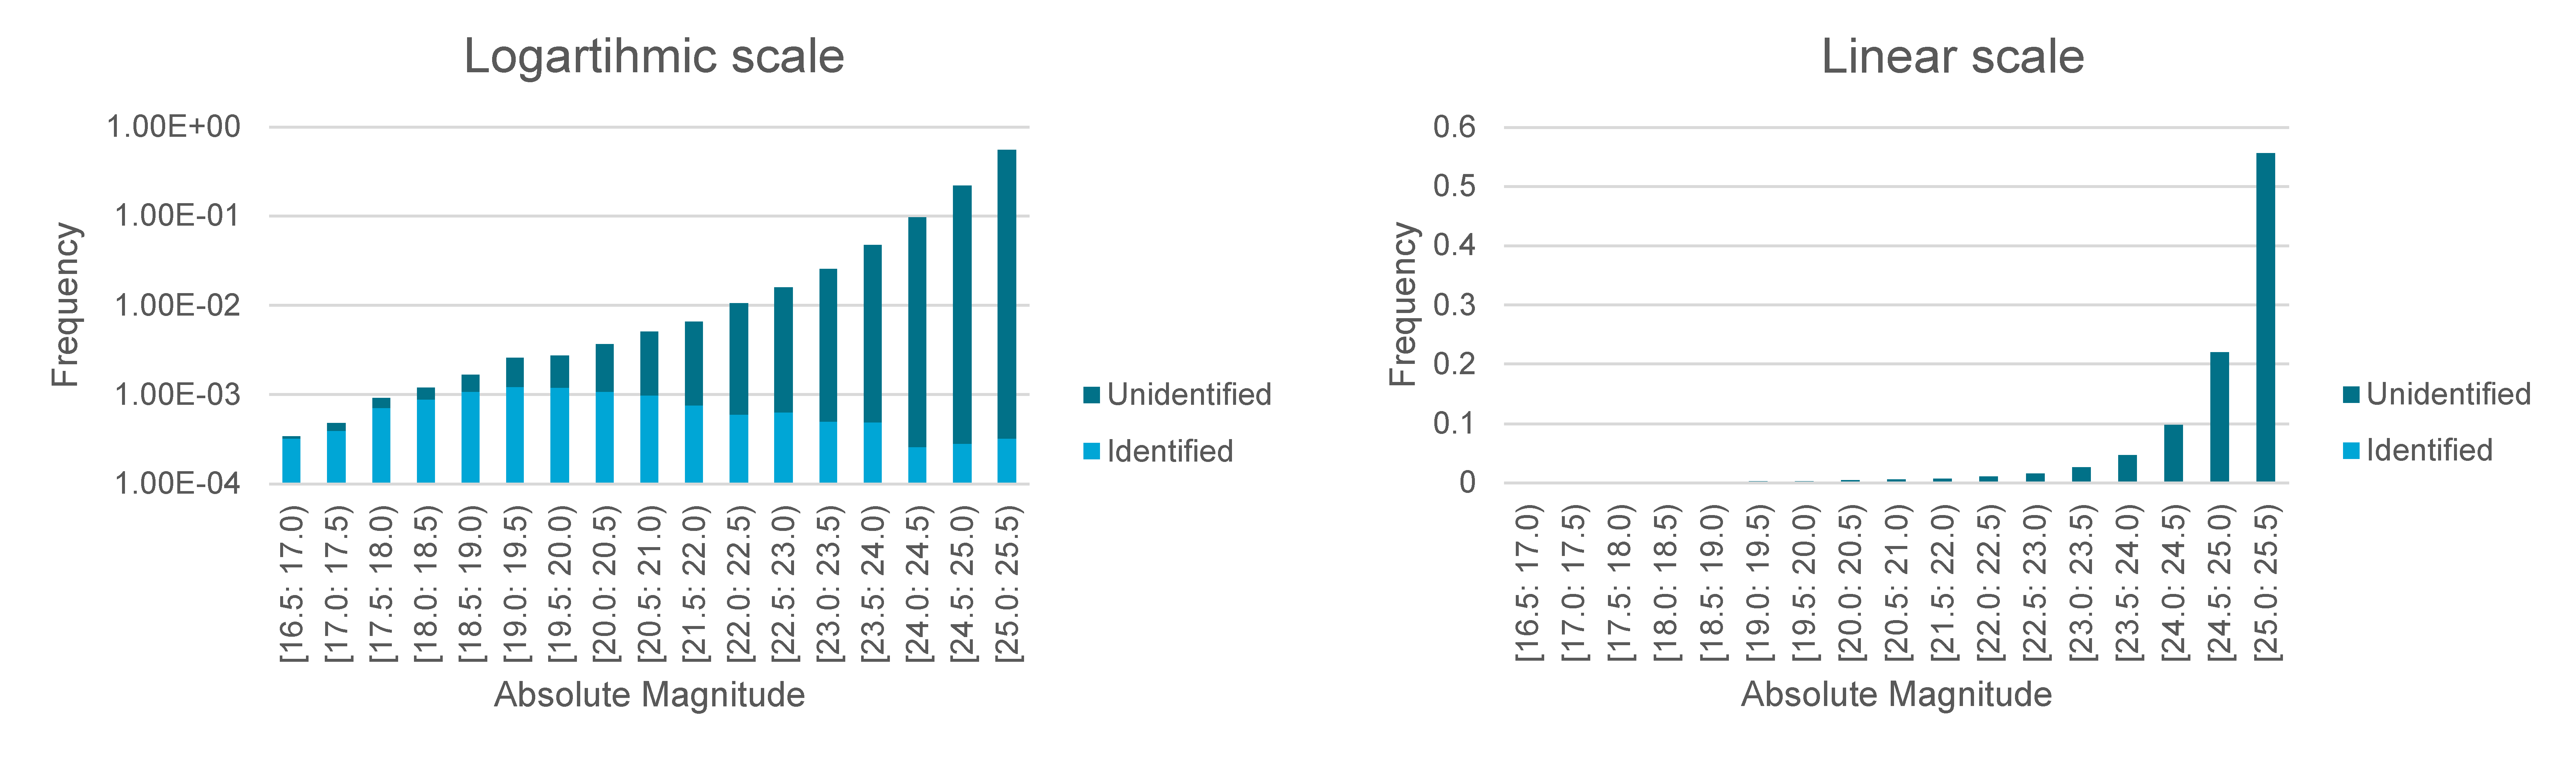
\includegraphics[width=1.0\textwidth]{img/population_identification_correction.pdf}
 \caption{Distribution of the full population of asteroids per \cite{GranvikPopulation}, and an estimation of how many asteroids have already been identified, per \cite{HarrisPopulation}. The left graph is shown logarithmically, the right graph uses a linear scaling.}
 \label{fig:populationcorrection}
\end{figure}


Of course, this results in a full population of NEAs; whereas a population of \textit{unidentified} NEAs is required for this work. Therefore, a correction to the population was made based on the work of \cite{HarrisPopulation}. To do this, the population as given by \cite{GranvikPopulation} was separated, based on absolute magnitude, into bins of width 0.5. Then, it was assumed that the detection of NEAs is roughly uniform over the orbital parameters. The completeness statistics of \cite{HarrisPopulation} can then be used to discard a part of the population as \textit{identified}. For example, assume there are 1000 asteroids in the $H=(21.0; 21.5]$ absolute magnitude bin. \cite{HarrisPopulation} predicts a completeness of 0.115 for this range. Thus, to correct for the known fraction of NEAs, 115 out of the 1000 asteroids are selected randomly, and removed from the population. This process is performed for every absolute magnitude bin between $H=16.5$ and $H=25.5$. The result of this process is shown in \autoref{fig:populationcorrection}. Of course, the assumption of uniformity in the detection of NEAs is false: highly eccentric NEAs, NEAs that are very dark, or NEAs with a large semi-major axis are more likely to be undetected. However, no data is available on this matter, and therefore no better alternative was deemed to be available. The error is judged to be sufficiently small: firstly, all simulations will be affected equally. Secondly, as can be seen in the second diagram in \autoref{fig:populationcorrection}, only a small part of asteroids is discarded as the largest population groups by size have very low completeness numbers.

\section{Background Signal}
\label{sec:modelling_background}
Before considering the existing knowledge on modelling asteroid signals, first the background in which these targets has to be observed is discussed. In this section, the current relevant body of knowledge on modelling this background signal will be given. The background signal will be split into two components. Firstly, the background light originating from the Sun. This manifests most dramatically in the form of direct sunlight. However, also reflections off of interplantary dust are important. This reflection manifests in the phenomena of zodiacal light and gegenschein. The second component of the background signal, is the light from outside the Solar system. This light originates from other stars and manifests mainly as a diffuse background of starlight. Particularly, a very large concentration of this starlight is found around the galactic plane. \\

\begin{figure}[htbp]
 \centering
 \includegraphics[width=1.0\textwidth]{img/referenceframes.png}
 \caption{Illustration of the utilized reference frames. Also shown are the Sun, spacecraft, ecliptic plane (incl. vernal equinox), and Milky Way.}
 \label{fig:referenceillustration}
\end{figure}


The reason for separating the background signal into these two components is straightforward: in a reference frame fixed among the stars, the background signal from outside the Solar system is practically unchanging as the spacecraft moves around the Sun; the parallax of moving several AU is negligible on galactic scales. In constrast, the contribution of light from our Sun is directly dependent on the position of the spacecraft with regards to the Sun. For the mathematical treatment of these signals, four reference frames are defined, which can be seen in \autoref{fig:referenceillustration}:

\begin{itemize}
 \item \textbf{A heliocentric ecliptic reference frame} $e$: A right-handed reference frame whose principal plane is the eclpitic plane, origin at the center of the Sun, and the positive $X_e$-direction towards the vernal equinox.
 \item \textbf{A body-centered ecliptic reference frame} $b$: A right-handed reference frame whose principal plane is the orbital plane of the spacecraft, origin at the center of the spacecraft, and the positive $X_b$ direction towards the vernal equinox. Note that all orbits considered for the spacecraft lie in the ecliptic plane, and therefore this reference frame also has the ecliptic plane as its principal plane.
 \item \textbf{A body-centered ecliptic reference frame, oriented relative to the Sun} $h$: A right-handed reference frame defined similar to $b$, but with the positive $X_h$-direction towards the center of the Sun.
 \item \textbf{A galactic reference frame} $g$: A right-handed reference frame whose principal plane is the plane of the Milky Way, origin at the center of the Sun, and positive $X_g$-direction towards the galactic core.
\end{itemize}


The transformations between heliocentric ecliptic longitude and latitude $(l_e, b_e)$ and galactic longitude and latitude $(l_g, b_g)$ involve a series of rotations, and therefore require some reference values. With $b_{NGP}$ the latitude of the North Galactic Pole, approximately equal to $29.81^\circ$ or $0.5203 \mathrm{rad}$; ascending node of the Galaxy $l_{NGP}$, approximately $270.02^\circ$, $4.712 \mathrm{rad}$; and longitude of the galactic core $l_{GC}$, approximately $6.38^\circ$, or $0.1114 \mathrm{rad}$ (\cite{SkyBrightness}), the transformations are given by \cite{SkyBrightness} as follows:

\begin{align}
 b_g &= \sin ^{-1} (\sin b_e * \sin b_{NGP}) - \cos b_e \sin b_{NGP} \sin (l_e - l_{NGP} \\
 \sin l_g' &= \frac{\sin b_e \cos b_{NGP} + \cos b_e \sin b_{NGP} \sin (l_e - l_{NGP})}{\cos b_g} \\
 \cos l_g' &= \frac{\cos (l_e - l_{NGP}) \cos b_e}{\cos b_g} \\
 l_g &= \begin{cases}
        \sin ^{-1} (\sin l_g') + l_{GC}; & \cos l_g' \geq 0 \\
        \pi - \sin^{-1} (\sin l_g') + l_{GC}; & \cos l_g' < 0, \sin l_g' > 0 \\
        - \pi - \sin^{-1} (\sin l_g') + l_{GC}; & \cos l_g' < 0, \sin l_g' \leq 0
       \end{cases}
\end{align}

The transformation from the $e$ to the $b$ frame is simply a translation by the spacecraft coordinates $[x_e^{S/C}, y_e^{S/C}, z_e^{S/C}]$:
\begin{align}
 x_b &= x_e - x_e^{S/C} \\
 y_b &= y_e - y_e^{S/C} \\
 z_b &= z_e - z_e^{S/C}
\end{align}

Where $z_e^{S/C}$ will generally be zero as the spacecraft is located in the ecliptic plane. As the values of $[x_e^{S/C}, y_e^{S/C}, z_e^{S/C}]$ are negligible on galactic scales, the transformations from the spacecraft-fixed frame $b$ to the galactic frame $g$ are the same as the transformation from the heliocentric frame $h$ to the galactic frame. Lastly, the transformation from the body-centered frame $b$, to the body-centered frame oriented relative to the Sun $h$, involves a rotation around the $Z_b$-axis. As the latitude of the Sun in the $b$-frame is zero, the transformation is simply a subtraction of the longitude of the Sun in the $b$-frame, $b_b^{\odot}$ from the longitude in the $b$-frame:
\begin{align}
 l_h &= l_b \\
 b_h &= b_b - b_b^{\odot}
\end{align}

With the reference frames defined, the individual components can be discussed. Firstly, the contribution of the Sun will be discussed, and then the background starlight for both thermal infrared and visual light.

\subsection{Solar contribution}
Modelling of the thermal infrared background radiation as a result of the light from the Sun is described by \cite{IRDust}, based on observations of the COBE mission. This model focusses on a modelling of the thermal state of interplanetary dust, and the resulting thermal infrared emission observed. Thus, the signal is not comprised of light originating at the Sun - but rather on the radiation from bodies heated by that light. The authors state that the albedo of particles at the relevant wavelengths is very close to zero, and therefore scattered Sunlight needs not be considered; only the emissions of the particles. Thus, the zodiacal flux $Z(l, b)$ can be expresssed as an integral over the line of sight (in practice, a distance up approximately the orbit of Jupiter is sufficient) of the sensor of the various contributions (which will be discussed in  more detail below):
\begin{equation}
 Z(l, b) = \Sigma_c \int _{\lambda_0} ^{\lambda_1} \int _S n_{c}(X, Y, Z)  E_{c}(\lambda) B(\lambda, T) ds d\lambda
 \label{eq:irdustflux}
\end{equation}
With $n_c$ the density of the dust due to a contribution $c$, $B$ is the blackbody emission given by Planck's law and $E_c$ is a wavelength-specific emission correction factor. The temperature of the dust grains is assumed to follow a power law function of distance from the Sun $R$:
\begin{equation}
 T(R) = T_0R^{-0.467}
\end{equation}
Temperature $T_0$ at 1 AU is set to $286\mathrm{K}$, and the emissivity modifications at the $4.9 \mu\mathrm{m}$ and $12 \mu\mathrm{m}$ thermal infrared wavelength are $0.997$ and $0.958$, respectively. Then, based on observations of the COBE mission, the authors construct a parametric model, based on three contributions. The first contribution is a ``donut-shaped'' dust cloud centered at the Sun, and inclined $2.03^\circ$ with respect to the ecliptic. This is the largest contributor to the density of interplanetary dust. Two more contributions which are modelled are a set of three dust bands, inclined at $0.56^\circ$, $1.2^\circ$ and $0.8^\circ$. Lastly, a circumsolar ring is modelled along the orbit of the Earth, which has a higher concentration around $10^\circ$ behind Earth in its orbit, as dust trails the planet due to its gravity. For conciseness, the exact model will not be described here in detail; interested readers can refer to \cite{IRDust}. An illustration of the contours of the components is seen in \autoref{fig:irdustcontributions}.\\

\begin{figure}[htbp]
 \centering
 \includegraphics[width=1.0\textwidth]{img/ir_dust_components.png}
 \caption{Isodensity contours of the interplanetary dust model, shown at a plane perpendicular to the ecliptic. F.l.t.r.: the dust cloud, dust bands, and the circumsolar ring. Units of the contours are $10^{-7} ~\mathrm{AU}^{-1}$ for the dust cloud, and $0.125\cdot10^{-7} ~\mathrm{AU}^{-1}$ for the bands and ring (\cite{IRDust}).}
 \label{fig:irdustcontributions}
\end{figure}

The combined density model is shown in \autoref{fig:irdustcombined}. As can be seen, the dust cloud is the largest contributor to the density of the dust cloud. With the density and temperature components known, the infrared background due to the interplanetary dust can be modelled. The only factor that needs to be added to this is the direct thermal radiation from the Sun, which can be obtained directly from Planck's law. \\

\begin{figure}[htbp]
 \centering
 \includegraphics[width=0.6\textwidth]{img/ir_dust_combined.png}
 \caption{Combined isodensity contour of the interplanetary dust in a plane perpendicular to the ecliptic (\cite{IRDust}).}
 \label{fig:irdustcombined}
\end{figure}

Combining all these components and performing the integration leads to the full contribution as a result of Solar radiation and interplanetary dust. An illustration of the signal can be seen in \autoref{fig:solartirbackground}. The contribution from the Sun, and the hot dust near the Sun, is the most important source. However, there is still a sizeable flux originating in the interplanetary dust throughout the Solar system.\\

\begin{figure}[htbp]
 \centering
 \includegraphics[width=1.0\textwidth]{img/background_tir_zodiac.png}
 \caption{Contribution of light from the Sun to the background signal in thermal infrared, in the body-fixed reference frame $b$, as seen from a spacecraft located at (-1, 0, 0) AU in the heliocentric frame $h$. Units are Megajansky per steradian, $1 \mathrm{MJy}{sr}^{-1} = 10^{-21} \mathrm{W}\mathrm{m}^{-2}\mathrm{Hz}^{-1}\mathrm{sr}^{-1}$, and the scale is clipped at $35 ~\mathrm{MJy}{sr}^{-1}$ for clarity.}
 \label{fig:solartirbackground}
\end{figure}

On the other hand, the background signal in the visual spectrum is more readily available. As it can be quickly and repeatedly measured from the surface of the Earth, early measurements of this signal exist. The components of the visual light background signal are tabulated by \cite{LightOfTheNightSky}, using data obtained from measurements. The resulting contribution from the Sun and Sunlight reflected off of interplanetary dust can be seen in \autoref{fig:solarvisbackground}. Next to the obvious contribution of the Sun and zodiacal light, the phenomenon of gegenschein can be observed in the middle of the plot. Although this is the point where target asteroids are at their brightest, it is also a point of increased background flux. The values as tabulated by \cite{LightOfTheNightSky} are only valid at a distance from the Sun of 1 AU. \cite{SkyBrightness} offer a correction factor to obtain the flux $F$ for changing heliocentric distance of the observer $R$ from the flux at 1 AU $F_{1~\mathrm{AU}}$ as follows:
\begin{equation}
 F(R) = F_{1~\mathrm{AU}}R^{-2.3}
 \label{eq:sunscale}
\end{equation}
This correction factor accounts for both the approximate decrease in interplanetary dust density when moving away from the Sun, as well as the decrease in solar flux. With these components, the Sun-dependent portion of the background signal is fully available for modelling. \\

\begin{figure}[htbp]
 \centering
 \includegraphics[width=1.0\textwidth]{img/background_vis_zodiac.png}
 \caption{Contribution of light from the Sun to the background signal in the visual spectrum, in the body-fixed reference frame $b$, as seen from a spacecraft located at (-1, 0, 0) AU in the heliocentric frame $h$. Units are $S10_\odot$ or solar-type stars of 10th magnitude per square degree. $1S10_\odot = 9.00\mathrm{W}\mathrm{m}^{-2}\mathrm{sr}^{-1}$. The scale is clipped at $1000 S10_\odot$ for clarity.}
 \label{fig:solarvisbackground}
\end{figure}


\subsection{Milky Way and Diffuse Starlight}

For the background signal originating from the Milky Way and other diffuse starlight, similar models exist for both the thermal and infrared and the visual light spectrum. By subtraction of the signal from the Sun, zodiacal light and gegenschein, the remaining portion of the background signal could be attributed to this component. The resulting models from \cite{IRDust} and \cite{LightOfTheNightSky} are shown in \autoref{fig:starstirbackground} and \autoref{fig:starsvisbackground}, respectively. Due to the research being more modern, and more computer and data storage resources being available at the time, the thermal infrared background model can be seen to be more detailed than the visual light spectrum model. However, other similarities, such as the light from the galactic core around $l_b = 270^\circ$ can be observed in both. Lastly, note that while the diffuse background starlight generally has a lesser magnitude than the emission and reflection of the interplantary dust, the Milky Way is brighter than the interplanetary dust in both spectra and thus warrants inclusion into the model. \\

\begin{figure}[htbp]
 \centering
 \includegraphics[width=1.0\textwidth]{img/background_tir_stars.png}
 \caption{Contribution of light from the Milky Way and diffuse starlight to the background signal in thermal infrared, in the body-fixed inertial frame $b$. Units are Megajansky per steradian, $1 \mathrm{MJy}{sr}^{-1} = 10^{-21} \mathrm{W}\mathrm{m}^{-2}\mathrm{Hz}^{-1}\mathrm{sr}^{-1}$, and the scale is clipped at $35 \mathrm{MJy}{sr}^{-1}$ for clarity.}
 \label{fig:starstirbackground}
\end{figure}

A final note is to be made about individual stars: readers who occassionally glance at the night sky are undoubtedly familiar with the fact that numerous stars outshine the diffuse background, making them appear as individual, distinct points. Naturally, these point will also appear in images taken of the sky. Similarly, large features such as distant galaxies or nebulae will contribute higher concentrations of background signal. However, as these objects are essentially fixed with regards to the movement and timescale of human surveying efforts, they have been extensively catalogued. Therefore, treatment of the signal from these objects is a fairly straightforward and well-understood process (see \cite{StarRemoval} for a thorough explanation). Even if an NEA was to pass in front of such a source, as the mean signal of the source is known, the contribution of the target can still be extracted. Therefore, it is not required to include these objects in the analysis explicitly: their effect is included in the resulting Poisson noise from the background signal.

\begin{figure}[htbp]
 \centering
 \includegraphics[width=1.0\textwidth]{img/background_vis_stars.png}
 \caption{Contribution of light from the Milky Way and diffuse starlight to the background signal in the visual spectrum, in the body-fixed inertial frame $b$. Units are $S10_\odot$ or solar-type stars of 10th magnitude per square degree. $1S10_\odot = 9.00\mathrm{W}\mathrm{m}^{-2}\mathrm{sr}^{-1}$. The scale is clipped at $1000 S10_\odot$ for clarity.}
 \label{fig:starsvisbackground}
\end{figure}


\section{Target Signal}
\label{sec:modelling_target}
In addition to modelling the background signal, the target signal has to be modelled. Although in reality the radiation emitted or reflected by an asteroid is dependent on many factors, including, but not necessarily limited to, its size, surface composition, shape, temperature and rotational motion, models exist which provide good approximations. As the asteroid population model from \cite{GranvikPopulation} gives a distribution of absolute magnitudes, the starting point of these models will also be the asteroids absolute magnitude, along with the position of the asteroid and the spacecraft relative to the Sun. \\

Firstly, for determining the emission of an asteroid in the thermal infrared, several models have been constructed in recent years. The original model for asteroids in thermal infrared is provided in the work of \cite{AsteroidSTM}. However, more recently \cite{AsteroidNEATM} have given an updated model of the thermal emissions of asteroids, and therefore their Near-Earth Asteroid Thermal Model (NEATM) is considered the standard at time of writing. \\

The NEATM assumes asteroids to be spherical, nonrotating bodies in thermal equilibrium with the radiation emitted by the Sun. The night side of the asteroid is assumed to have a temperature of $0~K$. The equilibrium temperature is modelled as follows:
\begin{align}
 T(\phi) &= \begin{cases}
            T(0) \cos ^{1/4} \phi;& \phi < 90^\circ \\
            0;& \phi \geq 90^\circ
           \end{cases} \\
T(0) &= \left[(1-A)F_{\odot}/(\eta \epsilon \sigma)\right]^{1/4}
\end{align}
With $\phi$ the angular distance from the subsolar point, $A$ the bond albedo, $F_{\odot}$ the incident solar flux, $\epsilon$ the emissivity, $\sigma$ the Stefan-Boltzmann constant and $\eta$ the so-called \textit{beaming parameter}, a correction factor for the emission dependent on the non-sphericalness of the surface, which can be calibrated from observations. For the NEATM, this value is set to $\eta = 1.22$.\\

With the temperature distribution known, the emission can be determined through integration of Planck's law over the visible hemisphere. For this, the size of the asteroid needs to be determined, which can be done using \autoref{eq:asteroidsize}. Estimation of this albedo using current data is difficult, and therefore the previously mentioned value of $p_v = 0.14$ is assumed. Of course, this calculation is sensitive to the assumed value of the albedo. A future system utilizing both visual and thermal infrared measurements could use this dependancy on albedo to calculate the asteroid's size \textit{and} albedo, instead of only the absolute magnitude by comparing the target's signal in the visual spectrum (which is dependent on size and albedo), to the signal in the thermal infrared (which is only dependent on the size). This might lead to better estimates of these values in the future.\\

Calculation of the target signal in the visual spectrum is more straightforward, as no integration is needed; a simple phase equation is readily available to obtain the apparent visual magnitude $V$, as detailed by \cite{2003NEOSDT}:
\begin{align}
 V &= H + 5 \log r \Delta - 2.5 \log \left[ (0.85) \Phi_1 + 0.15 \Phi_2 \right] \\
 \Phi_1 &= e^{-3.33\left(\tan \frac{\alpha}{2} \right)^{0.63}} \\
 \Phi_2 &= e^{-1.87\left(\tan \frac{\alpha}{2} \right)^{1.22}}
\end{align}
For solar elongations less than 60 degrees, \cite{2003NEOSDT} suggest using a modified equation instead:
\begin{equation}
 V = H + 5 \log r \Delta + 5.03 - 10.373 \log (\pi - \alpha)
\end{equation}
In these equations, $H$ is the absolute magnitude, $\alpha$ is the solar phase angle, $r$ is the distance from the Sun to the target and $\Delta$ is the distance from the observer to the target. By definition, the ratio between a flux $F_2$ and a reference flux $F_1$ can be determined from the difference in their apparent magnitude $\Delta V$:
\begin{equation}
 \frac{F_2}{F_1} = 100^{\frac{\Delta V}{5}}
\end{equation}
As the Sun has an apparent magnitude of $V_\odot = -26.74$, and a flux of $F_\odot = 1361 \mathrm{W}\mathrm{m}^{-2}$ at 1 AU, the visual flux of the target $F_t$ can be calculated from its apparent magnitude $V_t$ as follows:
\begin{equation}
 F_t = F_\odot 100^{\frac{-26.74 - V_t}{5}}
\end{equation}
It is here where part of the difficulty of detecting very small NEAs becomes apparent: relative to a $D = 3.5 \mathrm{km}$ asteroid ($V \approx 15$), a $D = 350 \mathrm{m}$ asteroid ($V \approx 20$) only results in 1/100th of the flux, and a $D = 35 \mathrm{m}$ asteroid ($V \approx 25$) will only give off 1/10,000th of the flux in both spectra. Note also that there is no \textit{inherent} advantage to either method in detecting small NEAs when considering the target signal. However, the thermal infrared background signal is relatively smaller relative to the target signal (\cite{2003NEOSDT}).

\section{Hardware Properties and Signal-to-Noise Ratio}
\label{sec:modelling_hardware_SNR}

In addition to the signal properties, the hardware used to image the target is also of interest. Some of the properties of the hardware can then be used to compute the signal-to-noise ratio (SNR) of the target, and several other properties will be used in the next section to determine the search strategy and cadence. \cite{2017NEOSDT} gives a description of representative hardware for current and upcoming space survey telescopes. The overview can be seen in \autoref{tab:hardwareproperties}. For the thermal infrared, a HgCdTe detector is utilized, for the visual light a silicon CCD. \\

\begin{table}[htbp]
\centering
\caption{Representative hardware properties for space-based survey telescopes. (\cite{2017NEOSDT})}
\label{tab:hardwareproperties}
\begin{tabular}{ll|ll}
\textbf{Parameter}        &  & \textbf{Thermal Infrared} & \textbf{Visual Light} \\ \hline
Aperture &{[}m{]}            & 0.5                       & 0.5                   \\
Field of view &{[}deg{]}     & 1.7 x 7.13                & 10.6 x 5.3            \\
Bandpass &{[}$\mu$m{]}       & 6 - 10                    & 0.4 - 1.0             \\
Integration time &{[}s{]}    & 150                       & 24                    \\
Quantum efficiency &{[}\%{]} & 65                        & 88                    \\
Dark current &{[}e-/s{]}     & 1                         & 0.00055               \\
Read noise &{[}e-{]}         & 22                        & 4
\end{tabular}
\end{table}

Two important observations should be made from the data in \autoref{tab:hardwareproperties}. Firstly, the visual light system has better specifications with regards to noise and quantum efficiency. This is due to the more advanced level of technology in CCD development compared to thermal infrared detectors. Secondly, the square angle subtended by the visual light sensor is almost five times as large as the thermal infrared sensor, and the required integration time is less than one sixth. The former factor is also due to discrepancies in technological development, the latter is a result of the weaker signal in the thermal infrared band. Together, these factors result in a sizeable decrease in survey cadence, which will be discussed in the next section. A last factor which is not shown in the table is the requirement for thermal infrared telescopes to be cooled to very low temperatures, to avoid the heat of the telescope itself interfering with the measurements. Visual light telescopes are not hindered much by their own temperature, as spacecraft at normal operating temperatures emit very little visible light. \\

The signal-to-noise ratio of the observation can then be calculated by dividing the signal in $e^-$ by the root-sum-square of the noise terms, assuming the noise terms to be independent (\cite{DetectionAndTracking}):
\begin{equation}
 SNR = \frac{S_t}{\sqrt{S_t + S_b + D + R^2}}
\end{equation}
The target signal $S_t$ and background signal $S_b$ can be calculated from the flux $F$ as follows (\cite{DetectionAndTracking}):
\begin{align}
 S_t &= \frac{1}{hc}A \tau k_f Q_e F_t \\
 S_b &= \frac{1}{hc}A \tau Q_e F_b
\end{align}
Here, $A$ is the telescope aperture, $\tau$ the integration time of the image, $k_f$ is the \textit{straddle factor}, a correction factor for the diffraction of a point source ($k_f \approx 0.9$), $Q_e$ the quantum efficiency, and $h$ and $c$ the Planck constant and speed of light, respectively. The background flux is obtained by summation of the components described in \autoref{sec:modelling_background}; the implementation of calculation of the target flux is described in the next chapter. in the direction of the target. The noise terms in the SNR equation are:
\begin{itemize}
 \item $\sqrt{S_t}$: the Poisson noise of the target signal.
 \item $\sqrt{S_b}$: the Poisson noise of the background signal. Note that the background signal itself can be subtracted fairly easy, and thus only the Poisson term has to be considered (see \cite{StarRemoval}).
 \item $\sqrt{D}$: the Poisson term of the dark current noise. The mean dark current can be removed through proper sensor calibration (see \cite{OpNav}).
 \item $\sqrt{R}$: the readout noise.
\end{itemize}

Thus, the SNR of every target can be calculated at any point in time from any telescope in space in both the thermal infrared and visual light spectrum.

\section{Search Strategy and Cadence}
\label{sec:modelling_cadence}
Next, it is important to consider how the telescope will conduct the survey. Of course, a telescope can not view in all directions simultaneously. Very little literature exists on setup and optimization of such search strategies. \cite{Cadence} provides some guidance based on the search strategy for the NEOCam mission. Essentially, the telescope performs a grid-like search, from north to south and west to east. Each section of the sky is revisited four times in a short time to allow for determining the direction of motion of targets, which aids in the precision of orbital determination. Thus, the number of images required to image the entire sky once, $n_{images}$ is approximately four times the solid angle of a sphere $\Omega = \frac{360^2}{\pi} = 41253\mathrm{deg}^2$, divided by the solid angle subtended by the image sensor's field of view $\Theta$:
\begin{equation}
 n_{images} = 4\frac{41253\mathrm{deg}^2}{\Theta}
\end{equation}
The time required per image $t_{image}$ is the summation of three terms: the integration time $\tau$, the settle time $t_{settle}$, and the slew time $t_{slew}$, where the latter can be approximated conservatively by taking the larger of the two dimensions of the image sensor, $\theta_1$, and dividing it by the slew rate $\dot{\theta}$:
\begin{equation}
 t_{image} = \tau + \frac{\theta_1}{\dot{\theta}} + t_{settle}
\end{equation}
The survey cadence (the time required to do one survey cycle of imaging the entire sky; i.e. a survey cadence of ten implies the telescope images the entire sky every ten days) is then given by:
\begin{equation}
 T_{survey} = n_{images}t_{image}
\end{equation}

From the previously stated hardware properties of the visual light telescope in \autoref{tab:hardwareproperties}, and assuming a slew rate of $\dot{\theta} = 0.5^\circ\mathrm{s}^{-1}$ and a settle time of $t_{settle} = 10 \mathrm{s}$ the following values are obtained:
\begin{align}
 \Theta &= 10.6 * 5.3 = 56.18\mathrm{deg}^2 \\
 \theta_1 &= \mathrm{max}(10.6, 5.3) = 10.6 \mathrm{deg} \\
 \tau &= 24 \mathrm{s} \\
 t_{slew} &= \frac{10.6}{0.5} = 21.2 \mathrm{s} \\
 t_{settle} &= 10 \mathrm{s} \\
\end{align}
Therefore:
\begin{align}
 n_{images} &= 4\frac{41253}{56.18} = 2938~\mathrm{images~per~survey~cycle}\\
 t_{image} &= 24 + 21.2 + 10 = 55.2~\mathrm{seconds~per~image}\\
 T_{survey} &= 2938 * 55.2 = 162,177.6~\mathrm{seconds~per~survey} \approx 1.88~\mathrm{days~per~survey}
\end{align}

Which, at a duty cycle of just over 90\% represents a fair assumption of the visual survey cadence of 2 days. Similarly, a survey cadence of 21 days was calculated for the thermal infrared system. Note that, as already alluded to in the previous section, the thermal infrared system has a far slower survey cadence, which will hinder the identification performance. Therefore, no system can yet be said to be superior: the thermal infrared system benefits from increased imaging performance, but a worse survey cadence.

\section{Detection and Identification}
\label{sec:modelling_identification}

From the signal-to-noise ratio, detection and identification can finally be established. Firstly, detection of the signal from the noise. As described by \cite{2017NEOSDT}, detection in processed images is a probabilistic process: At low SNR (SNR < 1), while detection is possible, the detection should be rejected because the probability of false detections becomes too high. Conversely, at high SNR (SNR > 5), detection becomes almost certain: the risk of false positives is so small that detection can be established aggressively. Modelling the process by a normal distribution allows for the intermittent range of SNR to be approximated by an integrated Gaussian. This distribution can be seen in \autoref{fig:snrgraph}. \\

\begin{figure}[htbp]
 \centering
 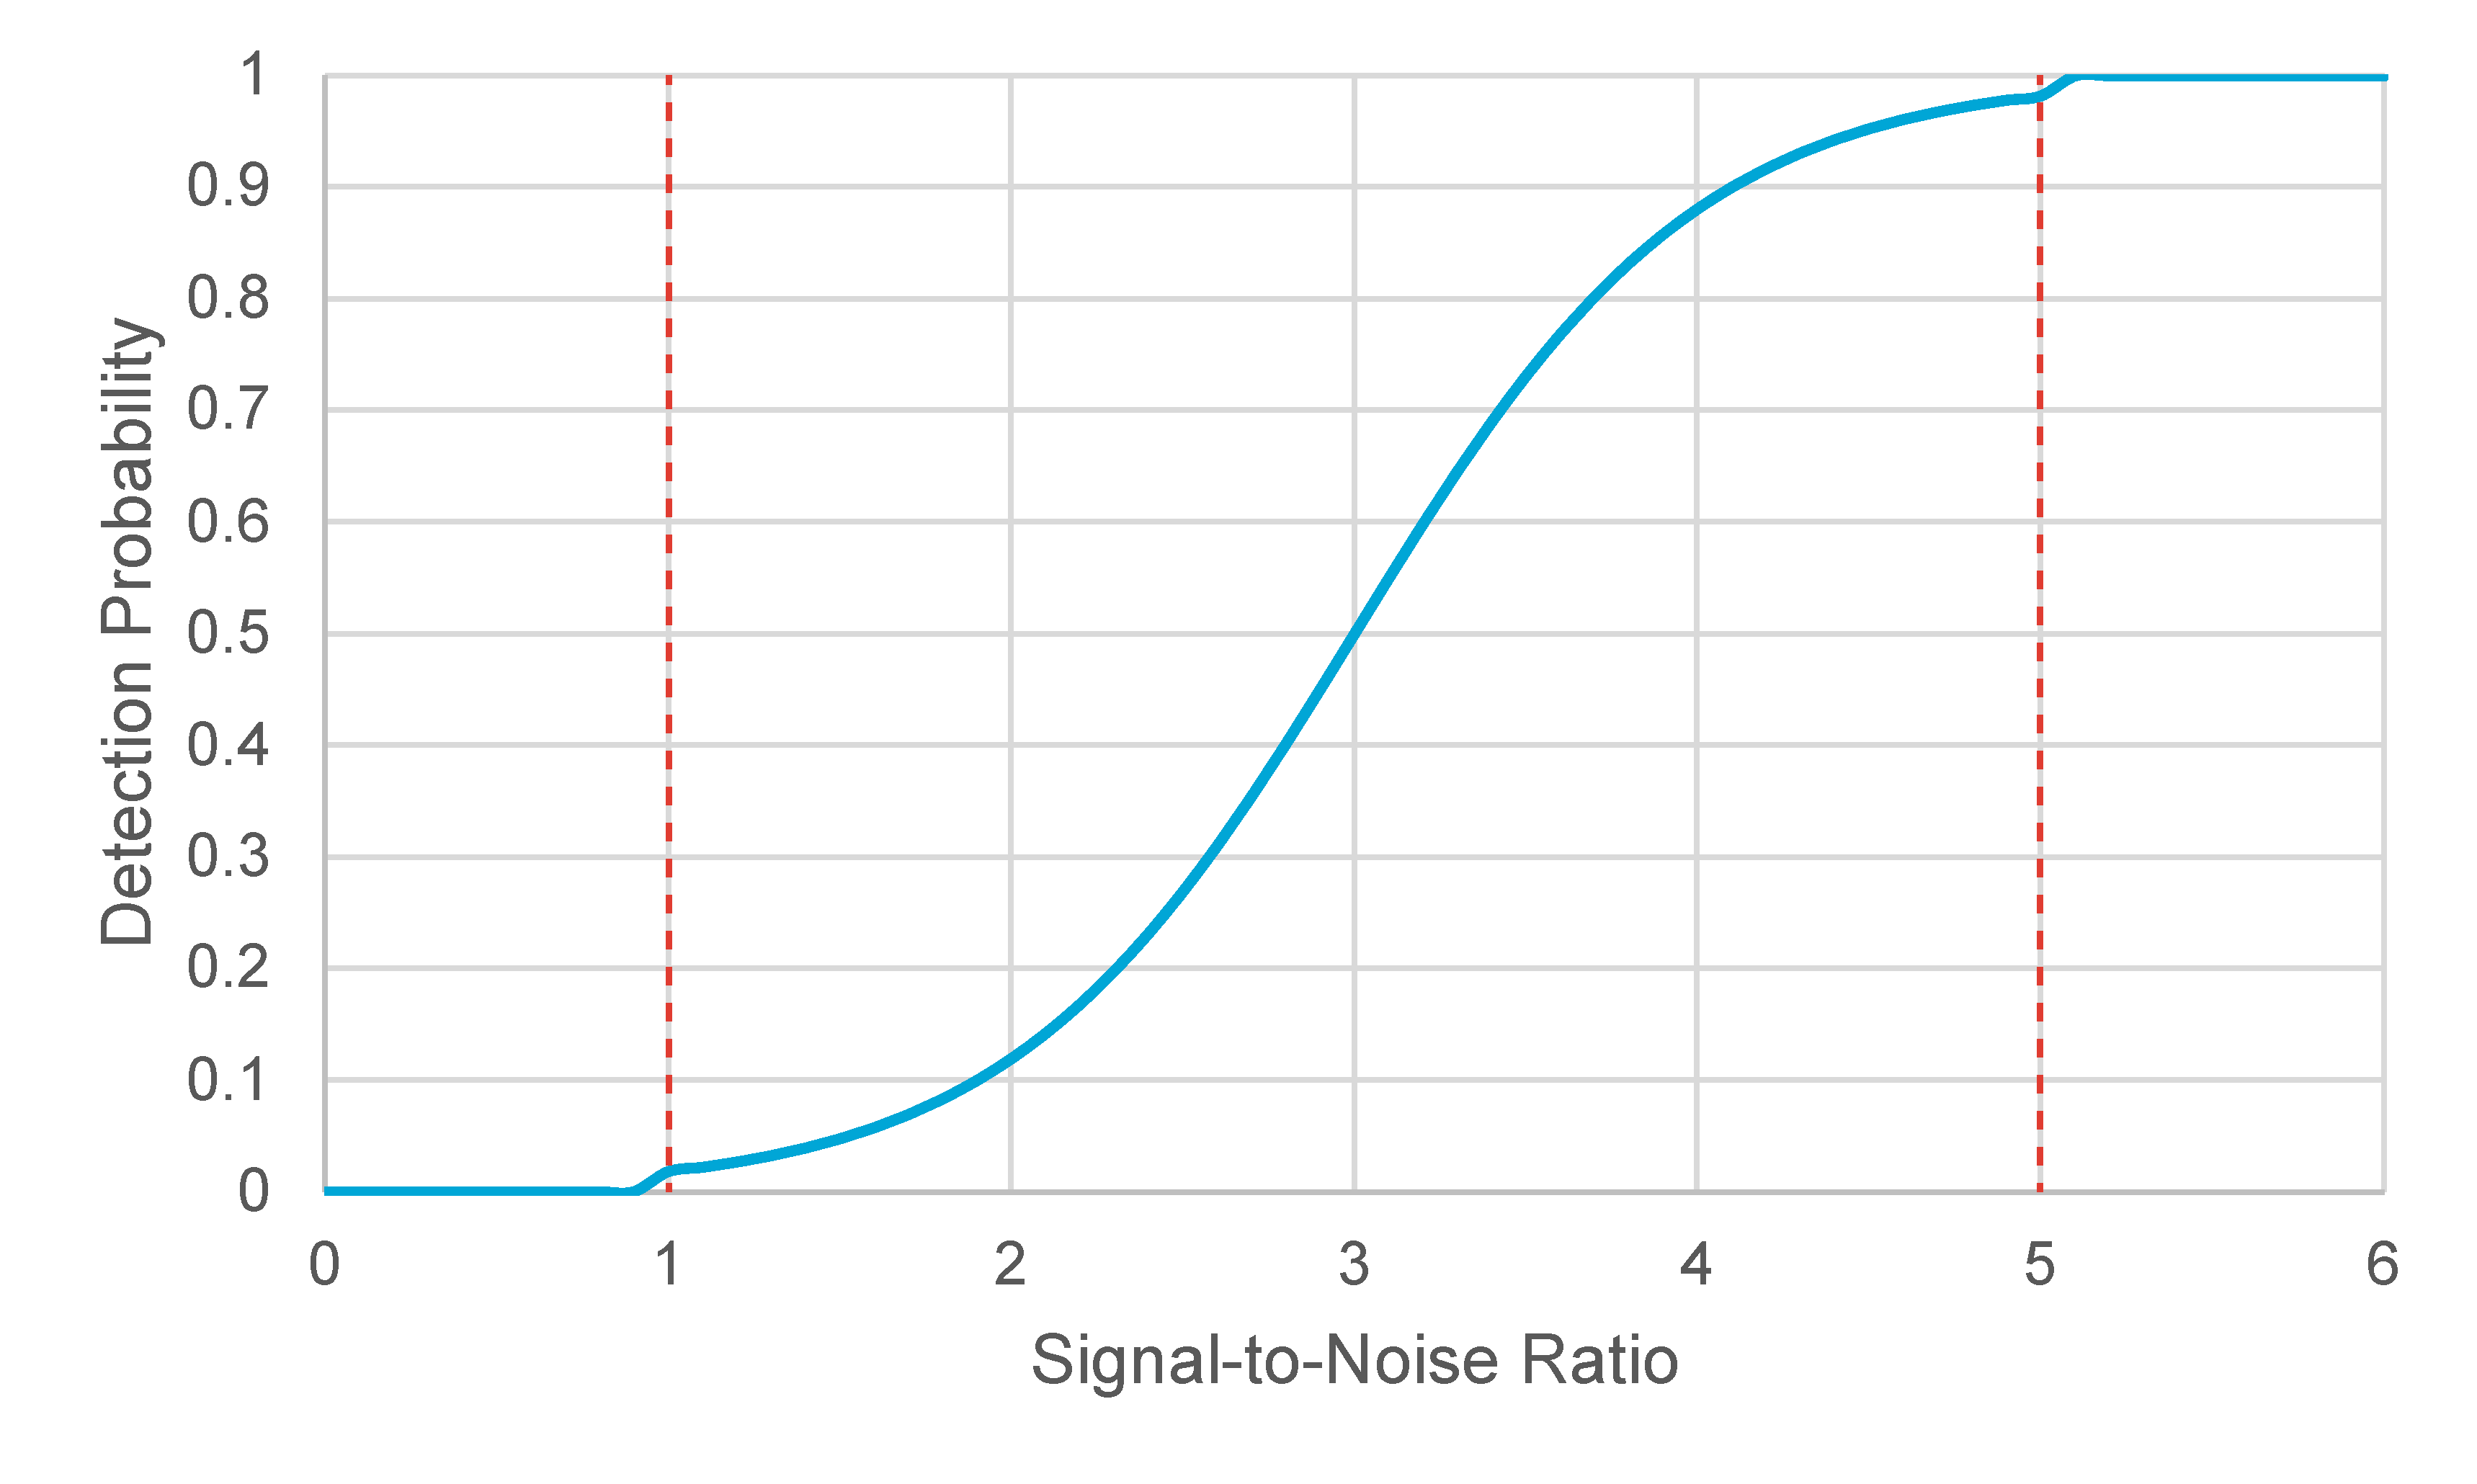
\includegraphics[width=0.7\textwidth]{img/snr_graph.pdf}
 \caption{Detection probability as a function of signal-to-noise ratio according to an integrated Gaussian. The function is truncated to 0 at SNR < 1, and to 1 at SNR > 5: at very low SNR, detection should be rejected as the possibility of false positives becomes too high; at very high SNR, the risk of false positives becomes so small that detection essentially becomes a certainty.}
 \label{fig:snrgraph}
\end{figure}

The process of identification is slightly more complicated. In essence, the process of solving for the orbit of a target asteroid using a single telescope uses Gauss' method, to obtain an orbit from three sets of angular measurements and the time between these. When multiple spacecraft are used and trangulation can be performed, two sets of positions and the time between these is enough to solve for the orbit, per Lambert's problem (see e.g. \cite{Curtis} for a thorough treatment of both methods). Theoretically, the time between these observations does not matter much, as long as the period is long enough to ensure that the curvature of the arc is larger than the uncertainty in the measurement (\cite{OpNav}). However in practice, the problem of \textit{linking} the observations arises: how does the system know that two observations spaced far apart in time belong to the same object? Currently, in practice, this results in a maximum time between subsequent observations ranging from 30 and 90 days (\cite{DetectionAndTracking}, \cite{2017NEOSDT}). However, it is expected that the resulting limit will be located more towards the maximum due to new techniques such as those presented by \cite{ShortArcs} and subsequent papers.\\

However, these methods rely on data being available throughout the system. It is currently unclear what data would need to be shared precisely, as no multi-spacecraft surveying systems have been researched to that level of detail to date. However, as \cite{2017NEOSDT} state, communication of survey results will be a point of attention for all deep-space surveying missions, not just multi-spacecraft ones, and an advanced communication system along with on-board data processing will be required. Luckily, modern techniques such as machine learning are being used to find computationally unintensive and simple solutions to the image processing pipeline (see, e.g., \cite{AIImage}). Therefore, this point will be considered to be out of scope of the research presented in this report. \\

With the detection and identification treated, a full overview has thus been presented of the process from obtaining the signal of both background and target, calculating the resulting SNR, and establishing detection and identification of NEAs. In the next chapter, implementation of these methods will be discussed.

\newpage
\chapter{Experimental Methodology}
After review of the background of near-Earth asteroid surveys and the existing body of literature for modelling surveys, this chapter will discuss the developed simulation in more detail. Firstly, in \autoref{sec::methdologysimulation}, the architecture of the simulation is discussed on a top-level. Then, in \autoref{sec:methdologyimplementation}, the implementation of the components of the simulation based on the literature in \autoref{ch:surveymodelling} is explained. Then, discourse will be given to the methods of optimization utlized in the research in \autoref{sec:methodologyoptimization}. Lastly, in \autoref{sec:methodologyprocess}, the process of using the simulation and optimization methods to obtain the results and conclusions presented in the next chapter is explained as well as the reasoning to support the optimization results. For reference, the interested reader can find the complete code as-is \href{https://github.com/ArjanVermeulen97/thesis/tree/main/code}{on Github.}

\section{Simulation Overview}
\label{sec:methodologysimulation}
First, before discussing the specifics of implementation, a general overview of the simulation is given. The objective of the simulation is to accurately predict the performance of a NEA survey by a given system of spacecraft, on a given population. Any optimization or validation is not considered a part of the simulation, but rather a system utilizing it. This will be further explained in \autoref{sec:methdologyprocess}.

\begin{figure}[htbp]
 \centering
 \includegraphics[width=0.7\textwidth]{img/simulation_overview.png}
 \caption{Overview of the simulation architecture and main loops.}
 \label{fig:simulation_overview}
\end{figure}

The architecture of the simulation is shown in \autoref{fig:simulation_overview}. On the top left, the main input parameters to the model are displayed. These are primarily the spacecraft and asteroid properties. Both of these consist of a full set of Keplerian orbital elements per spacecraft or asteroid. The asteroid properties furthermore include the albedo, size, and absolute magnitude of each asteroid; the spacecraft properties include which type of payload the spacecraft is carrying. \\

The simulation consists of a nested loop. Firstly, at the start of each timestep (the time between the timesteps is determined by the survey cadence), the positions of all asteroids and spacecraft are determined by propagation of their orbital elements. Then, in the inside loop, each spacecraft is checked against each asteroid to see if it can detect said asteroid. This is done through calculation of the signal-to-noise ratio (SNR). Lastly, as it is known which asteroids got succesfully detected by which spacecraft, it can be determined if asteroids have been identified. Then, at the end of the simulation, the result is a list of the asteroid population in addition to whether they have been detected, and if so, when. Of course, this data can be further processed.

\section{Implementation}
\label{sec:methodologyimplementation}
In this section, the implementation of the simulation algortihm is discussed. The simulation was written fully in Python 3.8, for reasons of easy testing and iteration, availability of packages for data handling and analysis, and familiarity of the author. The simulations were ran on several computers equipped with consumer-grade 6-core CPU's. \\

With regards to specific packages, data handling and computation was performed using \href{https://pandas.pydata.org}{Pandas} and \href{https://numpy.org}{NumPy}. Parallelization was performed using \href{https://dask.org}{Dask}. Critical paths of these packages are written in C/C++/Cython, vastly improving the performance of the simulation. Optimization was implemented through \href{https://pypi.org/project/scikit-optimize}{Scikit-optimize} and \href{https://scikit-learn.org/stable/index.html}{Scikit-learn}. Where necessary for the purpose of analysis, data visualisation was performed using \href{https://seaborn.pydata.org}{Seaborn}. Several other packages were used, but their exact functionality and specification is not relevant for the implementation and operation of the simulation.

\subsection{Population of Asteroids, Spacecraft, and Orbital Mechanics}
The population of asteroids was implemented based on the work of \cite{GranvikPopulation}. The authors \href{http://www.iki.fi/mgranvik/data/Granvik+\_2018\_Icarus}{provide an already generated population model} of 802,000 NEA's of absolute magnitude $17 < H < 25$. This saves having to implement and validate their modelling separately. For the simulation, a random sample of asteroids is drawn for each simulation run. It was found that a number of 1000 asteroids provided adequate accuracy while reducing computational load. For validation runs, 2500 asteroids were sampled instead to ensure a higher level of accuracy. The model includes for each NEA a unique identifier, a set of six keplerian orbital elements, the absolute magnitude, and the albedo. The data is implemented as a Pandas dataframe. Similarly, the spacecraft are also implemented as a Pandas dataframe, although their orbital elements and payload are given as input arguments to the simulation. \\

Orbits of asteroids and spacecraft were modelled using Keplerian orbits. As no complex mission gemetries or three-body interactions such as impacts are being studied, it was assumed that this would provide an accurate representation. The transcendental Kepler equation was solved numerically using the iterative method proposed by \cite{KeplerEquation}. Resulting orbits and transformations were verified manually. It is noted that calculation of the position of asteroids and spacecraft, especially solving of the Kepler equation, presents one of the largest contributors to the simulation's runtime. For future work, an alternative implementation is recommended.

\subsection{Background Signal}
Implementation of the background signal as described in \autoref{sec:modelling_background} was carried out as follows: Data for visual light is directly provided in the work of \cite{LightOfTheNightSky} in tabulated format for a longitude range of $[0^\circ, 360^\circ]$, in intervals of $10^\circ$. Latitude coordinates are provided in the interval $[-90^\circ, 90^\circ]$, in intervals of $10^\circ$. Additionally, latitude values of $-15^\circ, -5^\circ, -2^\circ, 2^\circ, 5^\circ, 15^\circ$ are provided for additional detail around the brightest areas (such as the galactic core or the Sun). Background signal originating from the Sun uses eclitic coordinates, signal from the background stars use galactic coordinates. After manual verification, the tables were saved. \\

The thermal infrared signal as described in \cite{IRDust} was implemented in two steps. Firstly, the thermal infrared background signal from outside the solar system was loaded, and the model for interplanetary dust and sunlight for the Sun-dependent portion of the background signal was implemented. For the latter, the required line-of-sight integration was performed numerically using a Riemann sum with a step size of $0.1~\mathrm{AU}$, up to a distance of $5.2~\mathrm{AU}$ from the Sun. Results were verified manually by inspection, and comparison of locations of well-known objects in the Milky Way to their locations in the background star signal. The latter step was taken to also ensure that the transformation from ecliptic to galactic coordinates was performed correctly. After verification, the resulting data was tabulated for the same longitude and latitude combinations as the visual light background signal. This was done to ensure universal operation of the code, reducing errors, and to avoid the computational load associated with processing the highly detailed \textit{COBE} data and performing the abovementioned numerical integration. \\

After tabulation, the background signal data can be held in memory during operation. Where necessary, it can be corrected to account for the spacecraft's distance from the Sun using \autoref{eq:sunscale}. When necessary, the value of the signal is determined from interpolation by means of Scikit's linear N-dimensional interpolator. \autoref{fig:combinedvisbackground} and \autoref{fig:combinedtirbackground} show the resulting background signal in the visual light and thermal infrared, respectively. It can be seen that some loss of detail in the thermal infrared is incurred due to the tabulation, however the effect is minor.

\begin{figure}[htbp]
 \centering
 \includegraphics[width=1.0\textwidth]{img/background_vis_combined.png}
 \caption{Background signal in the visual spectrum, in ecliptic coordinates, as seen from a spacecraft located at (-1, 0, 0) AU. Units are $S10_\odot$ or solar-type stars of 10th magnitude per square degree. $1~S10_\odot = 9.00~\mathrm{W}~\mathrm{m}^{-2}~\mathrm{Sr}^{-1}$. The scale is clipped at $1000 ~S10_\odot$ for clarity.}
 \label{fig:combinedvisbackground}
\end{figure}

\begin{figure}[htbp]
 \centering
 \includegraphics[width=1.0\textwidth]{img/background_tir_combined.png}
 \caption{Background signal in thermal infrared, in ecliptic coordinates, as seen from a spacecraft located at (-1, 0, 0) AU. Units are Megajansky per steradian, $1 ~\mathrm{MJy}~{sr}^{-1} = 10^{-21} ~\mathrm{W}~\mathrm{m}^{-2}~\mathrm{Hz}^{-1}~\mathrm{Sr}^{-1}$, and the scale is clipped at $35 ~\mathrm{MJy}~{sr}^{-1}$ for clarity.}
 \label{fig:combinedtirbackground}
\end{figure}

\subsection{Target Signal}
Implementation of target signal is a straightforward process. For the visual spectrum, the formulae listed in \autoref{sec:modelling_target} could be directly copied. The thermal infrared signal involves a triple integration, and is slightly more complex. As this process has to be performed $n_{asteroids} * n_{spacecraft} * T_{simulation} / \Delta t$ times per simulation, performance has to be taken into account when implementing the integrations. \\

Firstly, the integration of Planck's law over the bandpass. No closed-form solution exists for the definite integral of Planck's law. As Planck's law is relatively smooth, the decision was made to approximate the integral by the average of the start and end of the bandpass. In practice this means:
\begin{equation}
 \int _{6 \mu\mathrm{m}}^{10 \mu\mathrm{m}} B(\lambda, T) d\lambda \approx \frac{1}{2}\left[B(6 \mu\mathrm{m}, T) + B(10 \mu\mathrm{m}, T)\right] \Delta \lambda
\end{equation}
This essentially approximates Planck's law as a linear function in the domain. It is assumed that this is accurate for the range and temperatures considered. This simplification has to be made, as this integration has to be carried out for every part of the numerical integration over the visible hemisphere of the asteroid, and is thus performed even more often per simulation (in fact, it is the most-called function in the simulation). The integration over the visual hemisphere of the asteroid is performed by first assuming the asteroid to be a sphere. From geometry this integral is well known:
\begin{equation}
 F(x) = R^2\int_{-\pi/2}^{\pi/2}\int_{-\pi/2}^{\pi/2} f(x) \cos \theta \cos \phi d \theta d \phi
\end{equation}
This integration was implemented through a Riemann sum as well, using the midpoint rule and an interval of $\pi/4$ for both directions, resulting in a total of 16 evaluations. It was found that the error with respect to a very precise integration was less than 1\%. Examples of the implementation can be seen in FIGUREEEE


\subsection{Search Strategy and Cadence}
Implementation of the search strategy and cadence proved to be the most problematic aspect in the implementation process. As mentioned in \autoref{sec:modelling_cadence}, very little literature exists on the topic, and no methods have been developed to obtain an optimal search strategy utilizing multiple spacecraft. Several options were considered to model the strategy and resulting cadence. Firstly, a method omitting implementation, instead performing a correction ex post, such as utlized by \cite{ThesisOlga}. This method was expected to underrepresent the effect of a distinct survey cadence, and introduces a look-ahead bias which would both be very problematic for the acccuracy of the results of this simulation. Secondly, explicitly modelling a north-to-south, west-to-east gridsearch-like strategy such as described by \cite{NEOCam}. Although this model would arguably be the most accurate, it is very impactful with respect to the computational load, for three reasons:
\begin{itemize}
 \item Firstly, the positions of the asteroids and spacecraft have to be calculated for each imaging step. This results in calculating the positions $41,253 / (7.13*1.7) \approx 3400$ times for thermal infrared, or 734 times for the visual spectrum, for each complete scan of the sky.
 \item Secondly, to check whether or not an asteroid is inside the field-of-view of the telescope, trigonometric calculations are necessary, which are computationally inefficient.
 \item Lastly, the conditional logic required to select only asteroids inside the field-of-view prevents parallelization and vectorization of critical parts of the computation.
\end{itemize}
In addition, as mentioned previously, an optimized multi-spacecraft search strategy would not utilize such a methodology in reality either. Therefore, the claim to increased accuracy is not useful, and not neccessarily representative of how the real system would function. The last option considered, which was the one ultimately implemented, is discretization of the entire cadence into a single imaging step, essentially neglecting the search strategy altogether. In practice, this means that instead of modelling out the time per image, the entire timestep of the simulation becomes equal to the cadence, and all asteroids are imaged at the same time once in that interval. For example, for a thermal infrared system with an integration time of $150~\mathrm{s}$, and a survey cadence of $21$ days, this would mean that instead of taking one $7.13^\circ x1.7^\circ$ image every $150~\mathrm{s}$ of a select portion of the sky (one image at t=0, second image at t=150s, third image at t=300s etc.), one ``image'' is taken of the full sky every 21 days (one image at t=0, one image at t=21 days, one image at t=42 days, etc.). This might seem to induce a very large discretization error. However, the magnitude of this error is limited:
\begin{itemize}
 \item An asteroid might move out of the detectable range within the 21 day interval. In this case the assumption causes the asteroid to not be detected. However, conversely, an asteroid might also move into the detectable range in this time period. Assuming both phenomena to be approximately equally common, the error in predicted performance should be small.
 \item An asteroid might move in the direction of the imaging, causing it to be detected twice in two different fields-of-view, decreasing the time needed to identify the asteroid by providing a second observation within the 21 day window. Again, the converse might also happen with an asteroid being ``missed'' in this way. Although it might seem this error is therefore also negligible, it is actually not, as most bodies in the Solar system (including NEA's) orbit the Sun counter-clockwise, and therefore a counter-clockwise survey will have slightly more occurences of double detections than missed detections. Still, considering the relative velocity between the NEA and the spacecraft means that this will also be a rare process.
 \item Lastly, a quantization error is present due to the maximum window between observations (see \autoref{sec:modelling_identification}). Given e.g. a 90-day maximum period between observations, a discretized survey with a 21-day cadence virtually only has a window of 84 days, as the next observation occurs at t=105 days, and is thus outside the 90-day window. It is expected that this will lead to an underestimation of the survey performance, although the influence is also minor, as a repeat observation at 85 days < t < 90 days, when it was not possible to obtain two follow-up observations prior to this is rare, as the period between close approaches of the NEA and the spacecraft will be in the order of hundreds to thousands of days.
\end{itemize}
Although the above examples are given for a 21-day thermal infrared survey, it is also of note that the error will be significantly smaller in a visual light system due to the faster cadence. In addition, the error is expected to be roughly equal in magnitude for all simulations, and therefore will have little influence on the optimization process. Considering also the fact that this assumption will provide an estimated 5,000 - 10,000 times faster simulation, this implementation was selected as the best option. The actual effect of the assumption will be validated in REFFF


\subsection{Signal-to-noise, Detection and Identification}
Implementation of the SNR from the target signal, background signal, and hardware properties could be executed directly using the formulae presented in \autoref{sec:modelling_hardware_SNR}. However, the probabilistic detection model utilizes an integrated Gaussian distribution. As this has no closed-form solution, an approximation based on the hyperbolic tangent function (\cite{GaussianTanh}) was implemented. The function was only applied in the $1 > SNR > 5$ range. An SNR < 1 leads to an automatic failure in detection, and an SNR > 5 to an automatic success. \\

For identification, the number and period of the detections are tracked in the asteroid parameters dataframe. For reasons previously outlined, a maximum observation interval of 90 days was assumed. Two criteria can lead to a succesful identification:
\begin{itemize}
 \item Detection on three different timesteps within 90 days by at least one spacecraft. Note that it is not neccessary that all three detections are made by the \textit{same} spacecraft.
 \item Detection on two different timesteps within 90 days, by at least two spacecraft. Again, it is not necessary that these are the same spacecraft. In addition, it is assumed that the triangulation process is always possible: as the sensors have a pixel scale in the order of 1 arcsecond, colinearity is assumed to be a negligible phenomenon.
\end{itemize}

This means that all communication and image processing requirements are left out of the scope of the simulation. Such requirements, e.g. that the datarate between spacecraft is high enough that they can transmit observations to eachother, and that images can be processed on-board, would be design requirements for an eventual mission, such as also already outlined by \cite{2017NEOSDT}.

\section{Optimization Methods}
\label{sec:methdologyoptimization}
In order to obtain the optimal solutions to the problem, the simulation will be used in conjunction with a mathmatical optimizer. A plethora of optimizers exist to date, however a selection of promising optimization methods could be made fairly easily. Firstly, a large number of optimizers, the so-called gradient methods, are reliant on the availability of an analytical solution for the derivative of the function. No way of analytically evaluating the derivative of the simulation was found, and it is expected it does not exist due to the complexity. A second class of optimizers which is subsequently often considered are the heuristic-based methods, such as particle swarm optimization, simulated annealing, and genetic/evolutionary methods. However, these methods are firstly not guaranteed to find the global optimum, and secondly, require a very large number of function evaluations. Especially the latter is a problem, as the function is a full simulation, which is far from computationally trivial as shown in the previous sections. \\

Therefore, it was decided to implement a solution from the class of \textit{surrogate optimization} methods. In these methods, A more simple function is fit to the to-be-optimized function, and it is optimized instead as this allows using a more effective optimizer that can not be used on the function of interest, thereby limiting the number of required evaluations of the main function. The resulting queries to the main function are then used to update the surrogate function. As the surrogate function will eventually very closely resemble the main function, the method is guaranteed to approach the global minimum, provided the function is sufficiently smooth, can be evaluated in the entire domain, and does not have noise (\cite{Surrogate}).

\section{Experimental Process}
\label{sec:methodologyprocess}

\newpage
\chapter{Results and Discussion}
\label{ch:results}
The research process resulted in numerous interesting findings, with implications both for understanding the behavior of the system, as well as for future design efforts considering multi-spacecraft surveys. These results will be presented and discussed in this chapter. Firstly, the system's orbital elements, and how these are affected by the composition of the system, will be discussed in \autoref{sec:results_orbits_one} for spacecraft in co-orbital configurations. Afterwards, the effect of increasing or decreasing the number of spacecraft is discussed in \autoref{sec:results_number}. Then, possible payload compositions are assessed in \autoref{sec:results_payload}. To aid in the interpretation of these results, a possible explanation for the underlying principle is presented in \autoref{sec:results_explanation}. \autoref{sec:results_orbits_two} extends the analysis of the orbital parameters to non-co-orbital configurations, supported by the hypotheses on the underlying principles. Finishing the discussion, in \autoref{sec:results_performance}, predictions will be made with respect to the performance of an optimal multi-spacecraft survey system, and the impact on future design efforts will be discussed.


\section{Orbital Elements I: Co-orbital Spacecraft}
\label{sec:results_orbits_one}
Starting off, the orbital elements of the system are inspected. This is done both to find what the effect is of the orbital elements on the performance, but also how the payload and number of spacecraft affect the optimal orbital elements of the system. To facilitate analysis, and to later judge the results of the optimizer more accurately, the orbits are first analysed for a system of co-orbital spacecraft. That is, all orbital elements, except for the anomaly at epoch, are the same for all spacecraft. In addition, all spacecraft are spread out by an equal amount in terms of anomaly. This was done to vastly reduce the parameter space, and to reduce accidental overfitting to the population model. The latter follows from the fact that, logically, only the angular distance between the spacecraft should influence the result, not the absolute starting position, as the NEAs are distributed in a radially symmetrical fashion. I.e., a system with two spacecraft at mean anomaly at epoch $0$ and $\pi$ should give the same result as starting at $\pi/2$ and $3\pi/2$, only the inter-spacecraft distance is relevant.\\

\subsection{Semi-major axis}

\begin{figure}[htbp]
 \centering
 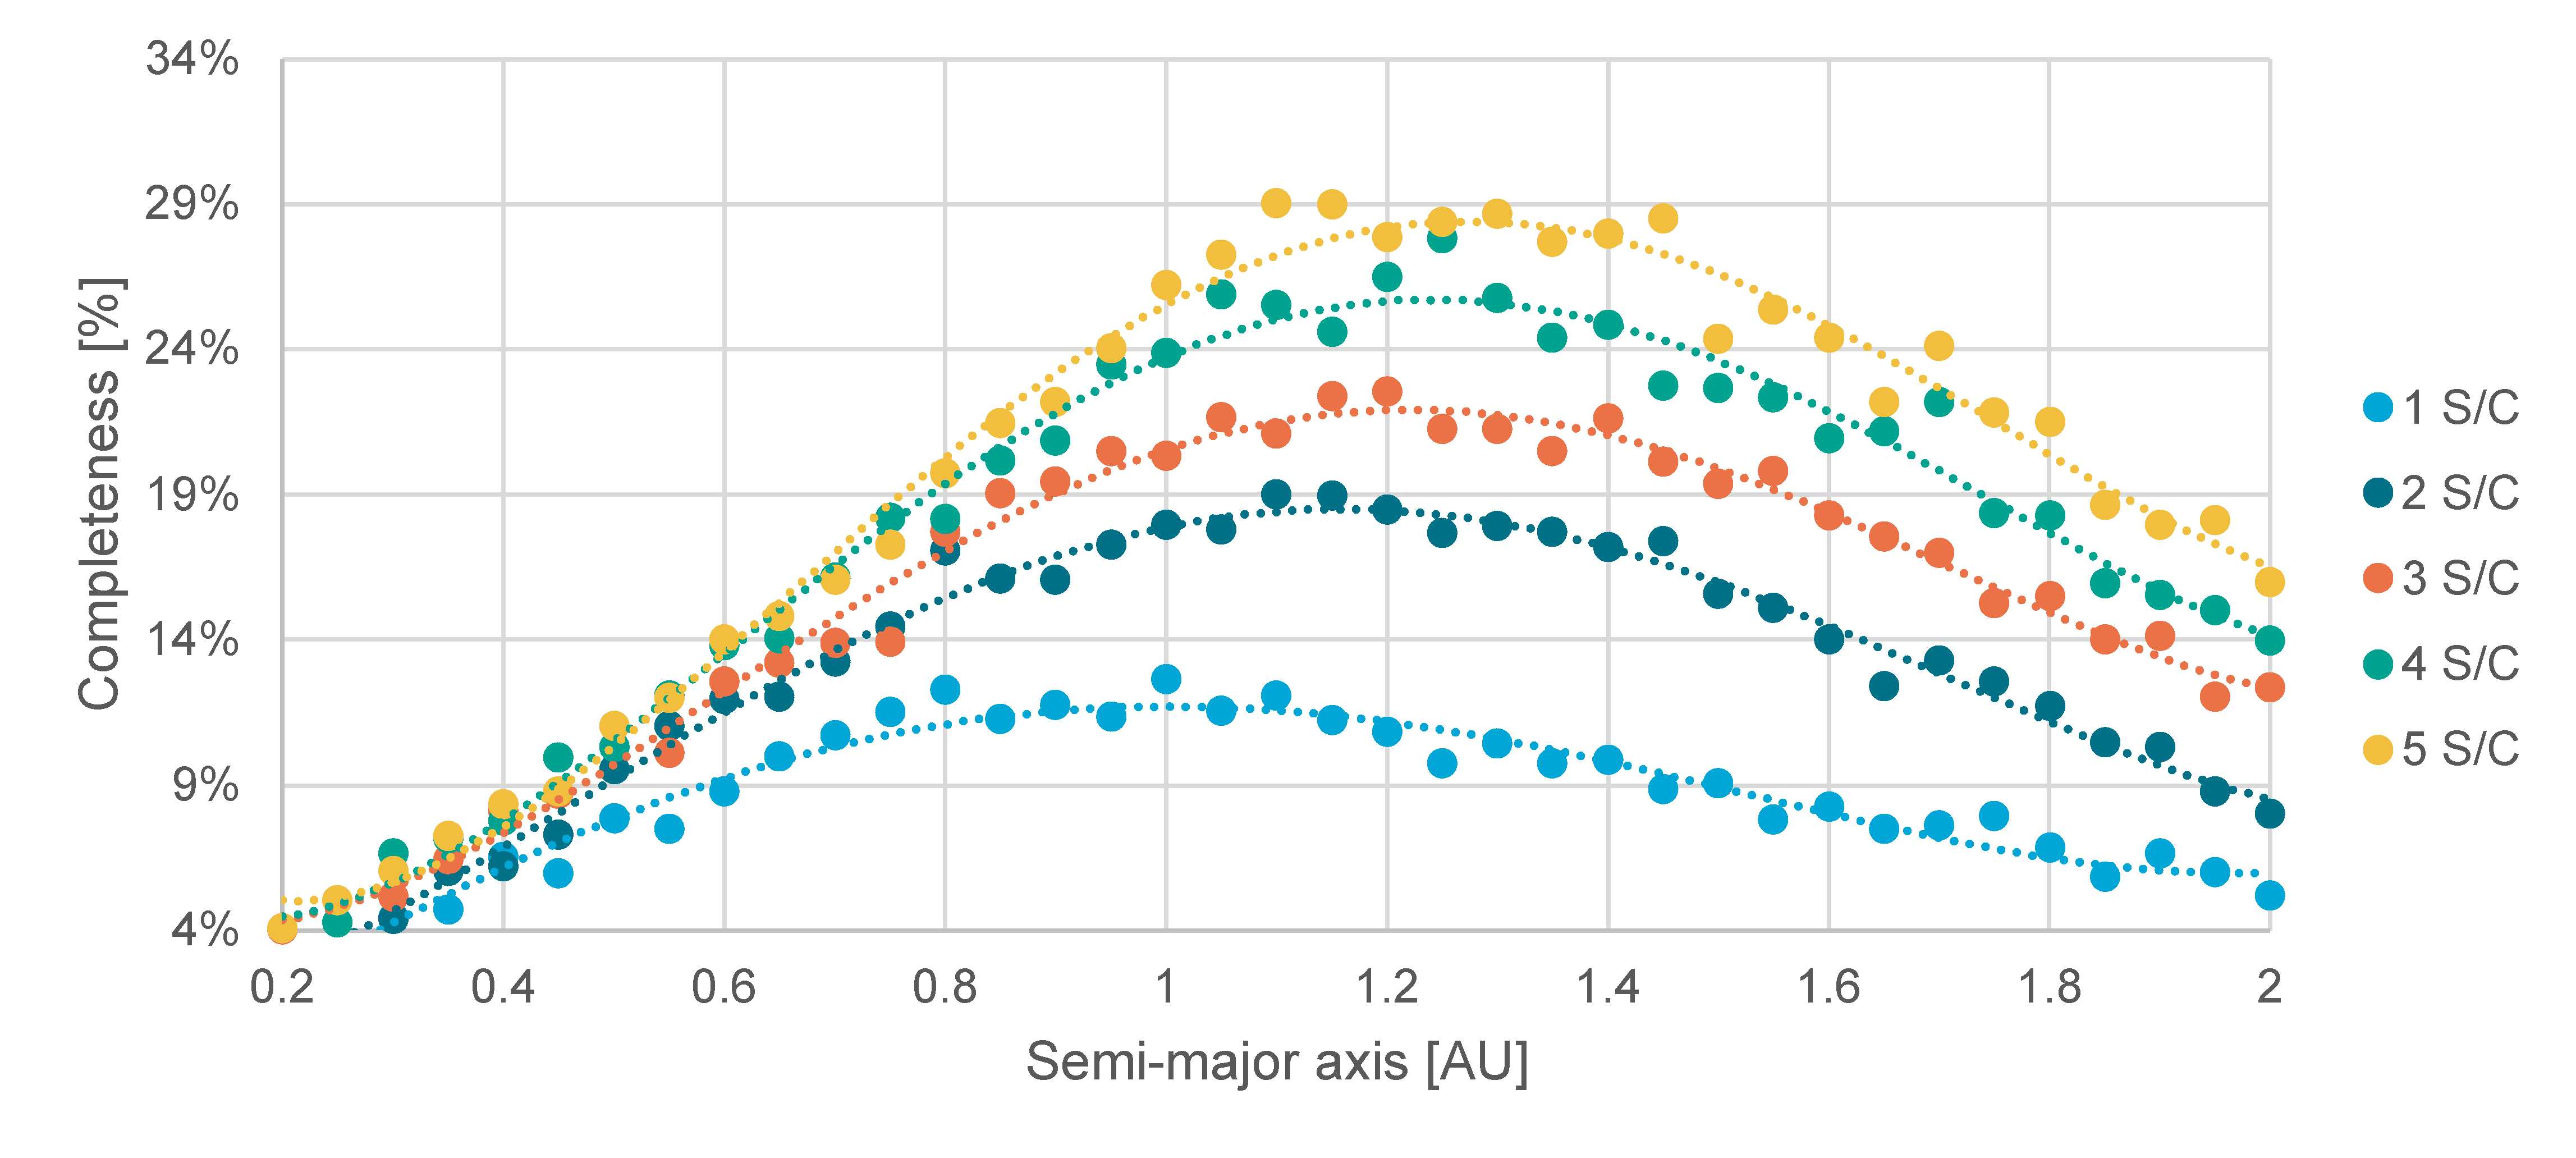
\includegraphics[width=0.8\textwidth]{img/vis_semi_maj.pdf}
 \caption{Visual light survey performance as a function of semi-major axis for 1 to 5 spacecraft. Corresponding eccentricity and angular separation of spacecraft are optimized using a grid search for each point.}
 \label{fig:vis_semi_maj}
\end{figure}

\begin{figure}[htbp]
 \centering
 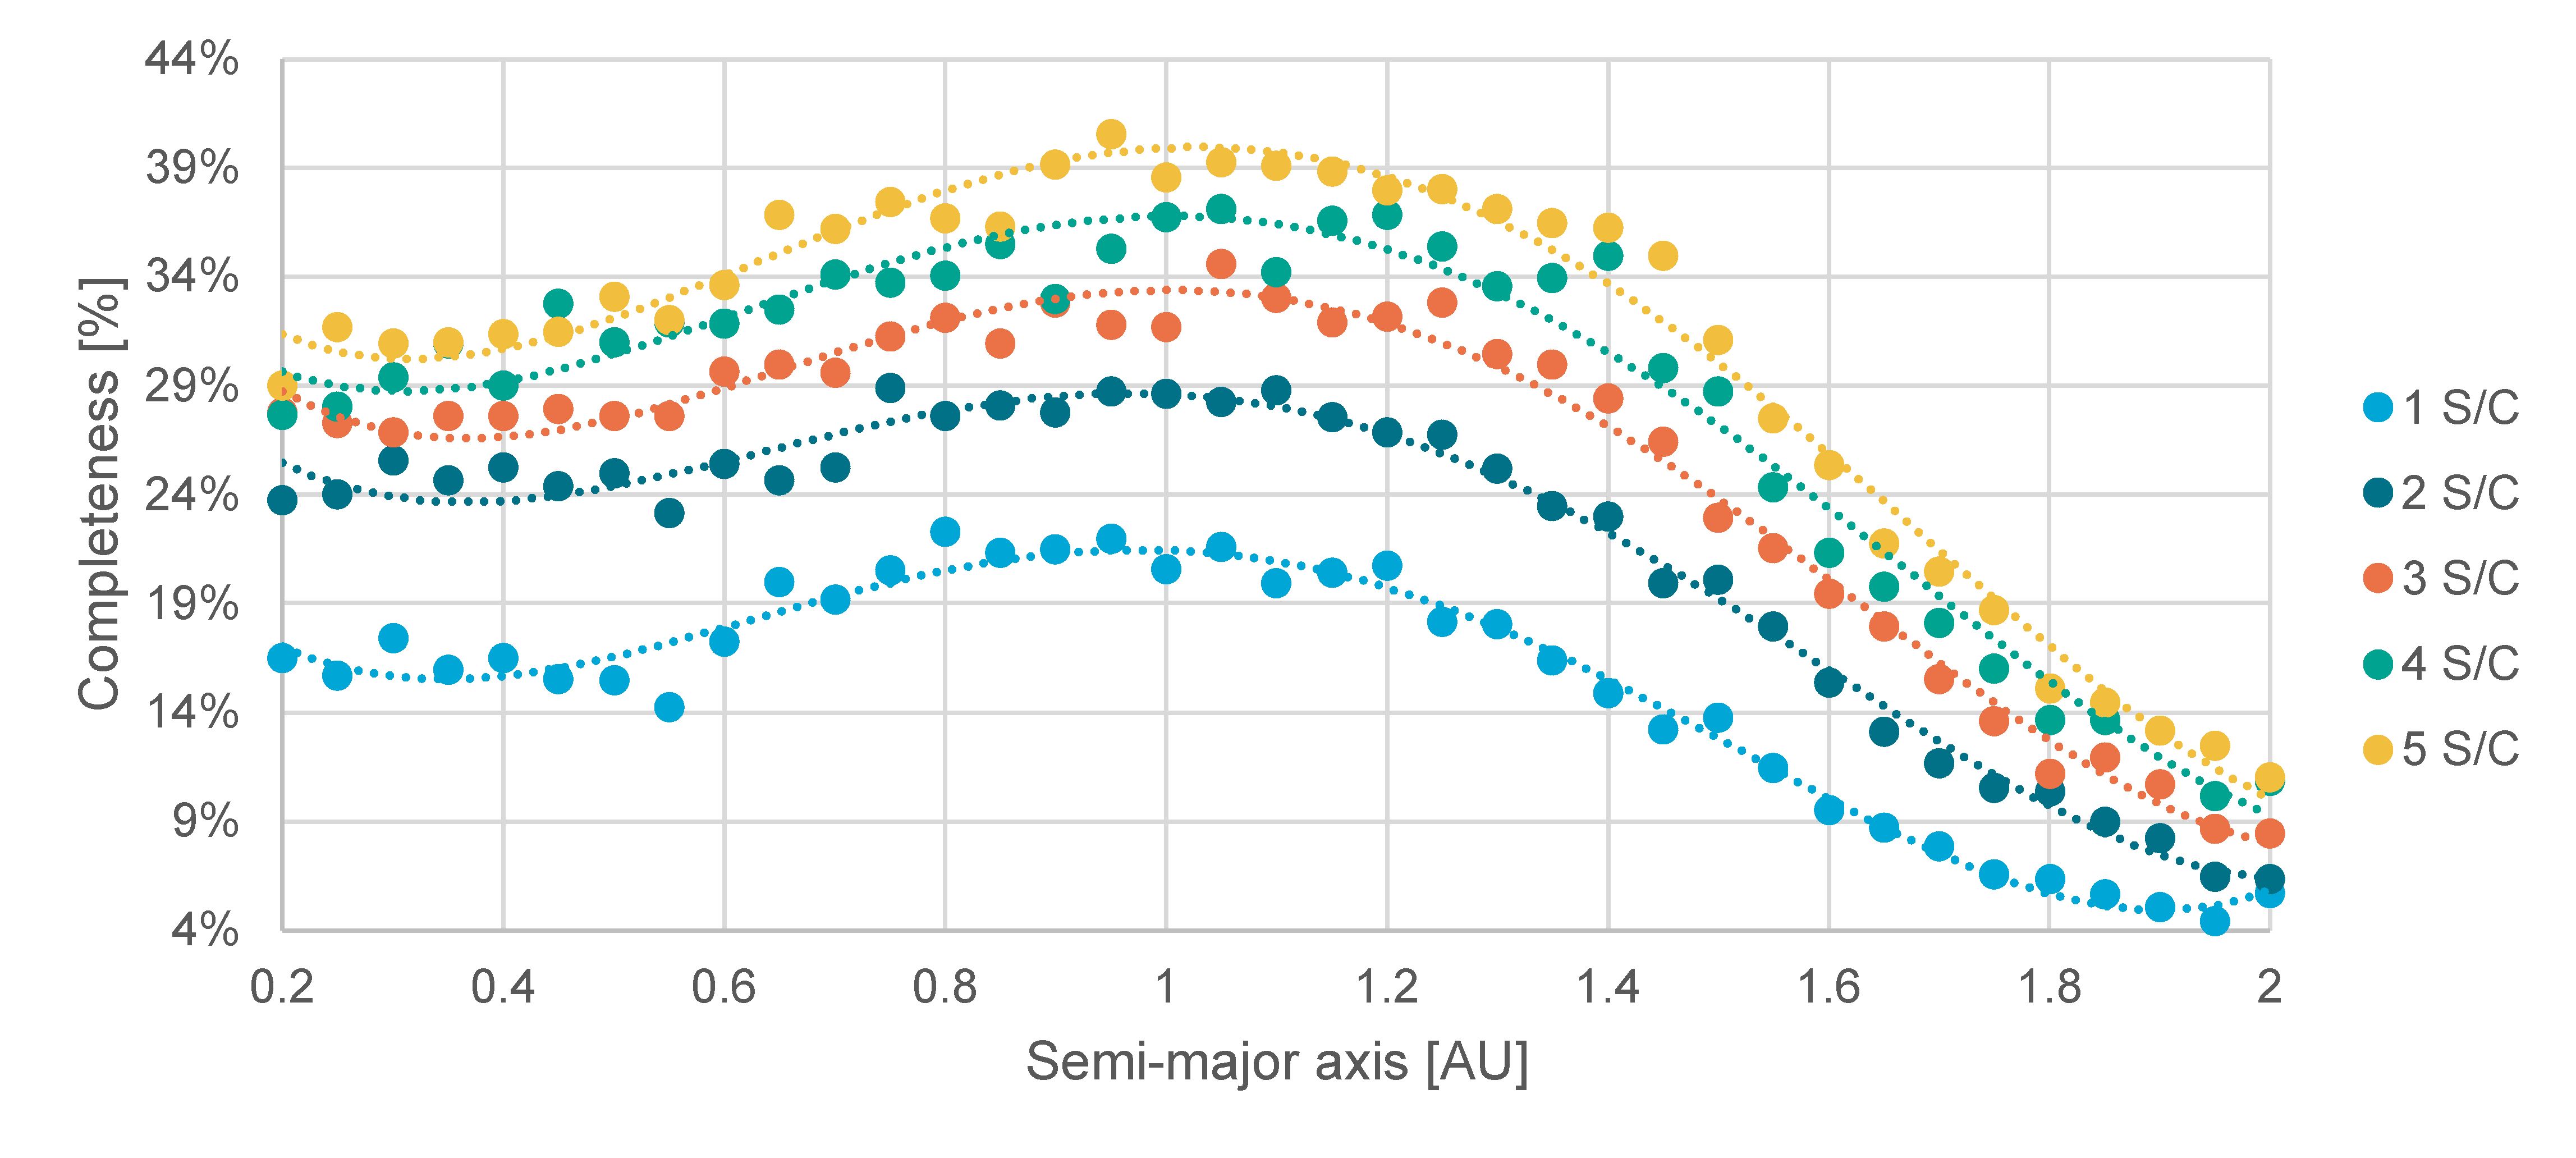
\includegraphics[width=0.8\textwidth]{img/tir_semi_maj.pdf}
 \caption{Thermal infrared survey performance as a function of semi-major axis for 1 to 5 spacecraft. Corresponding eccentricity and angular separation of spacecraft are optimized using a grid search for each point.}
 \label{fig:tir_semi_maj}
\end{figure}

In \autoref{fig:vis_semi_maj}, the expected survey performance as a function of semi-major axis is shown for visual light systems, and in \autoref{fig:tir_semi_maj} for thermal infrared systems. It can be clearly observed that the semi-major axis has an optimal value, which is dependent on the number of spacecraft. In addition, the region surrounding the optimum is very flat. Thus, locally, the solution is not sensitive to changes in semi-major axis up to a distance of approximately 0.1 AU from the optimum. There is however some variance present in the results due to the stochastic elements of the simulation. Two important conclusions are drawn here: Firstly, a wide range of semi-major axes lead to a well performing system. Secondly, due to the variance in results, it is difficult to pinpoint an exact optimal value. Therefore, in mission design, other considerations can and should be prioritized to determine a more precise semi-major axis. \\

The second factor of note is the change in the optimal semi-major axis as the number of spacecraft increases. It can be observed that increasing the number of spacecraft in the system leads to an increase in the optimal semi-major axis where the system should be positioned. This is further illustrated in \autoref{fig:semi_maj_function_of_n}, where the optimal semi-major axis is given as a function of the number of spacecraft explicitly. Here, it can also be seen that there is a large range of values possible for the semi-major axis. In addition, the semi-major axis becomes larger for higher numbers of spacecraft: E.g., a thermal infrared-equipped system comprising a single spacecraft should utilize a 0.9-1.0 AU orbit, but this increases to 1.0-1.1 for 3-5 spacecraft. Further increases in the number of spacecraft yield further increases. An explanation for this phenomenon is proposed in \autoref{sec:results_explanation}.

\begin{figure}[htbp]
 \centering
 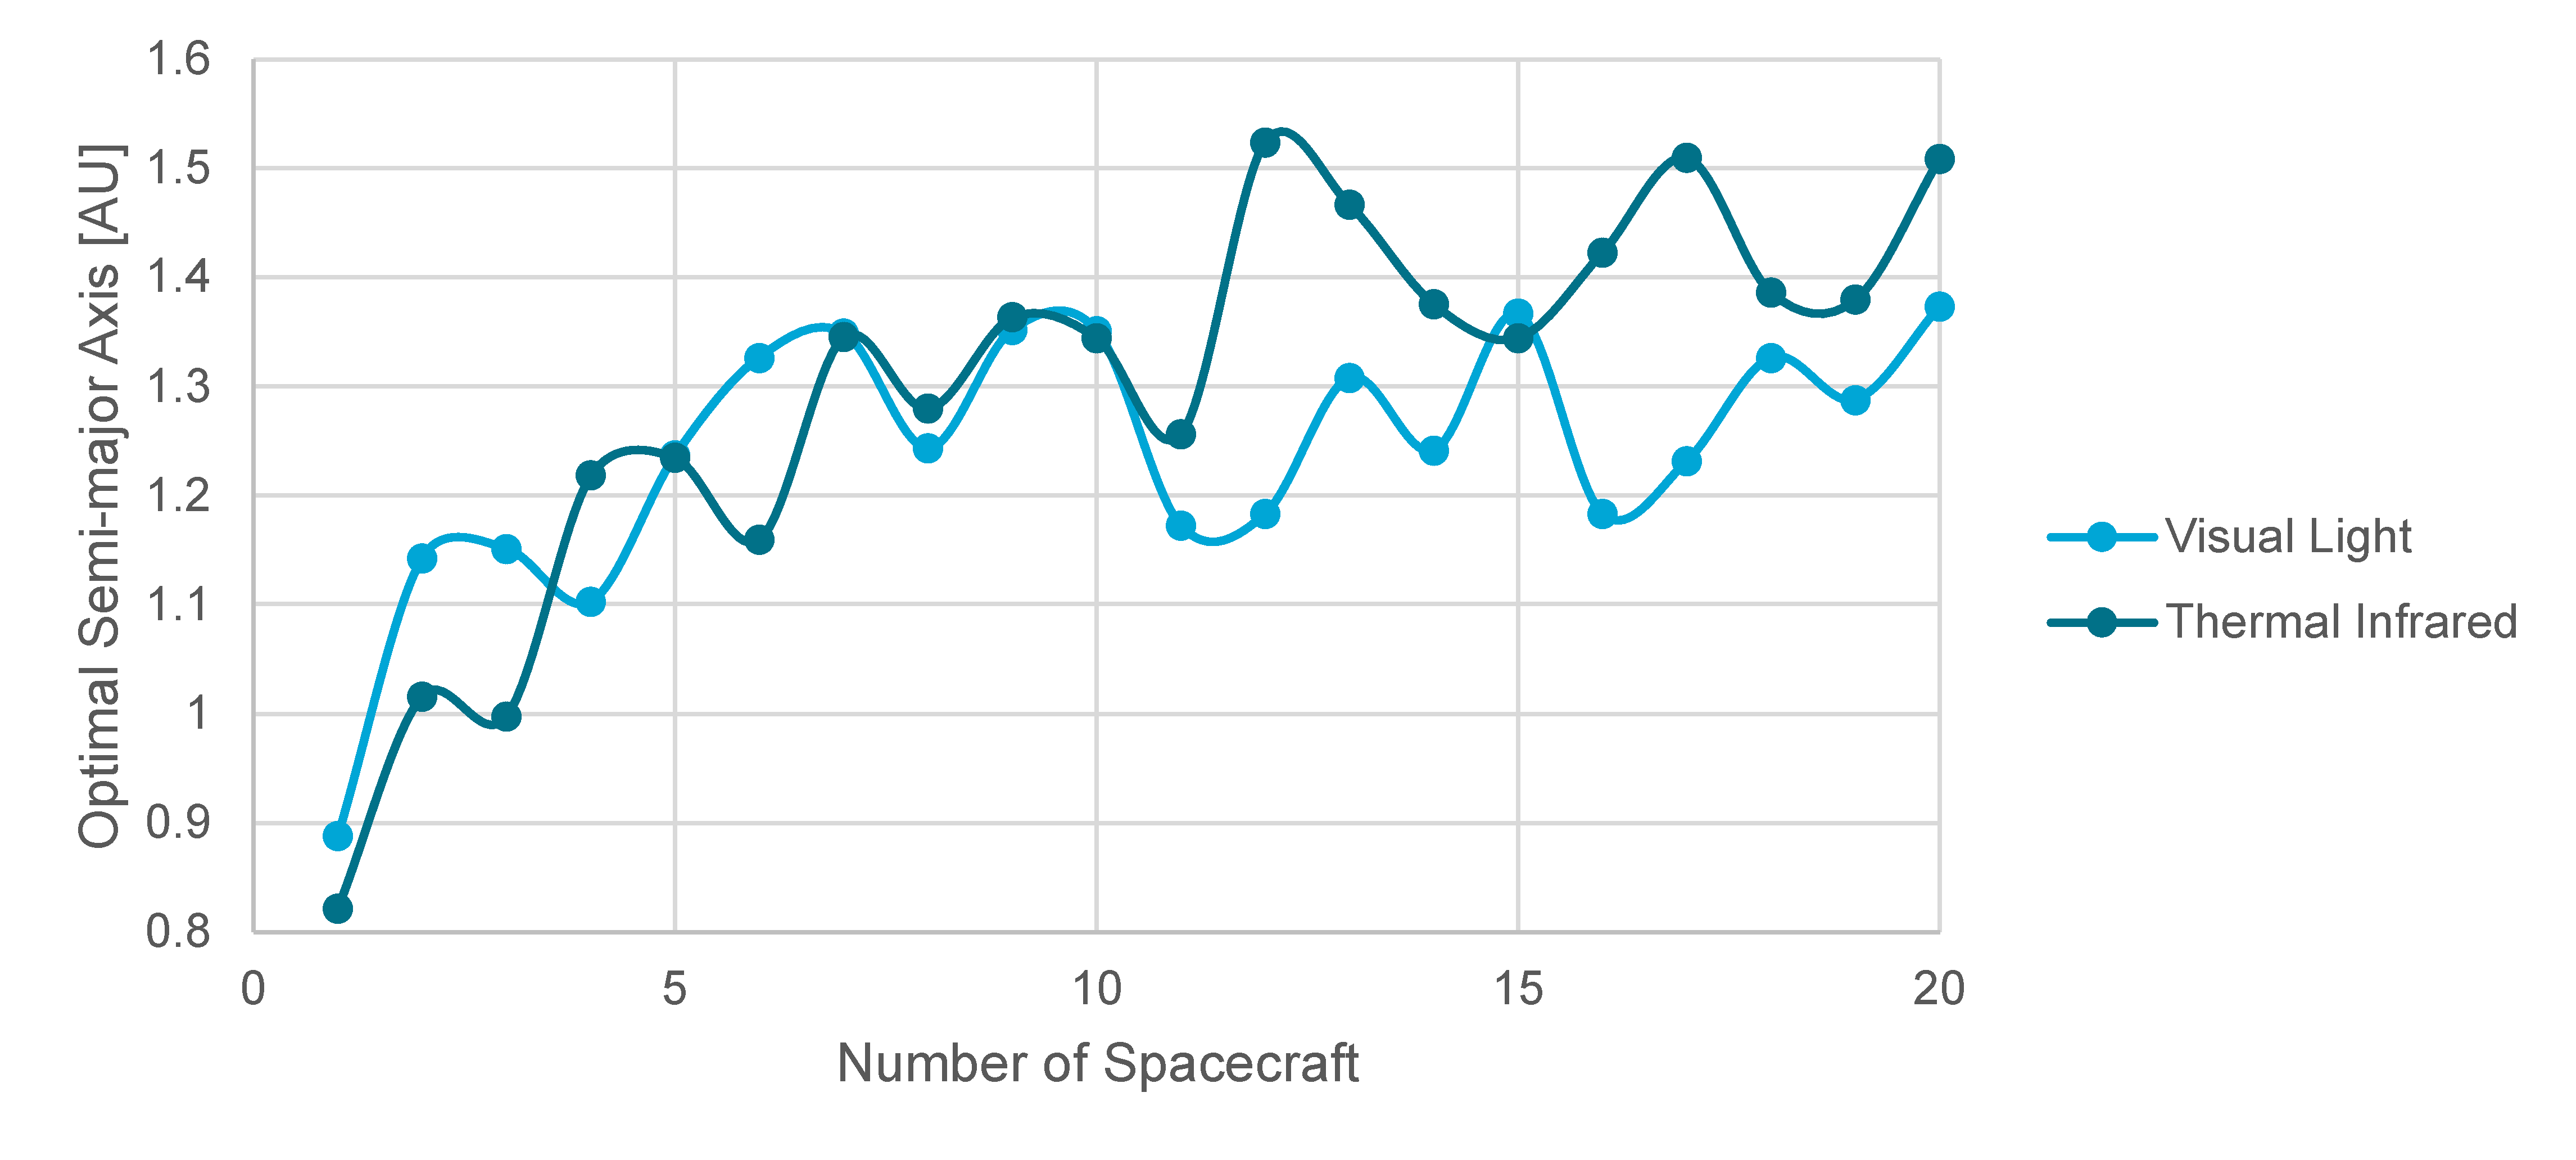
\includegraphics[width=0.8\textwidth]{img/semi_maj_function_of_n.pdf}
 \caption{Optimal semi-major axis as a function of the number of spacecraft in the system, including standard deviation bars. The eccentricity is zero, and the spacecraft are spread out equally. All values were optained using surrogate optimization, using 10 iterations to obtain the mean and standard deviation.}
 \label{fig:semi_maj_function_of_n}
\end{figure}



\subsection{Eccentricity}
\begin{figure}[htbp]
 \centering
 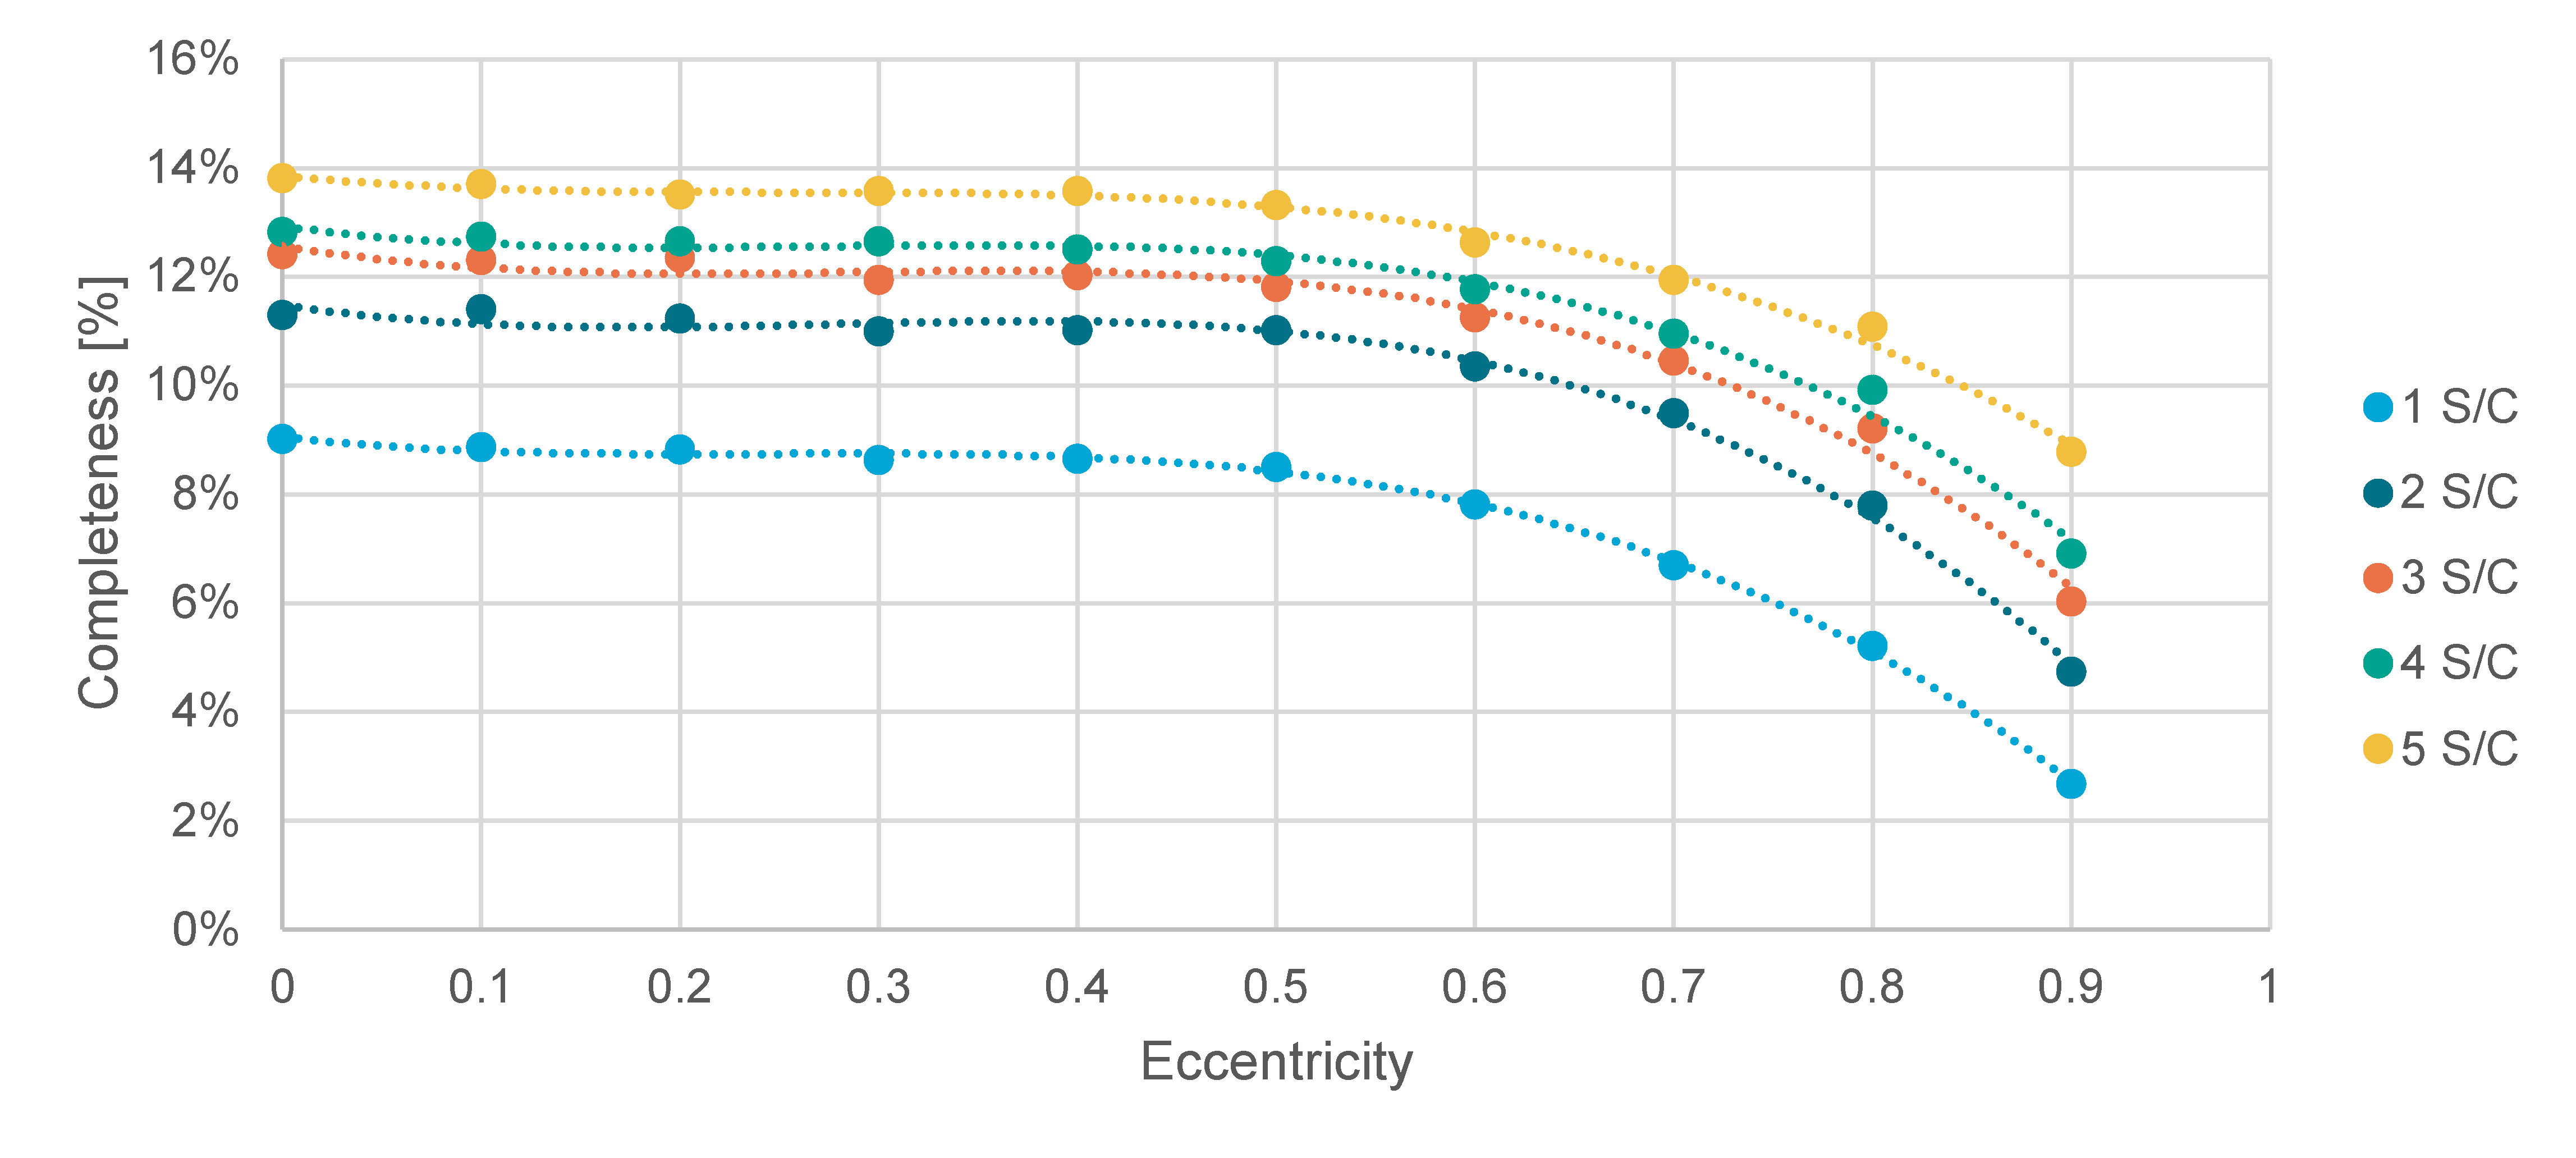
\includegraphics[width=0.8\textwidth]{img/vis_ecc.pdf}
 \caption{Visual light survey performance as a function of eccentricity for 1 to 5 spacecraft. Corresponding semi-major axis and angular separation of spacecraft are optimized using a grid search for each point.}
 \label{fig:vis_ecc}
\end{figure}

\begin{figure}[htbp]
 \centering
 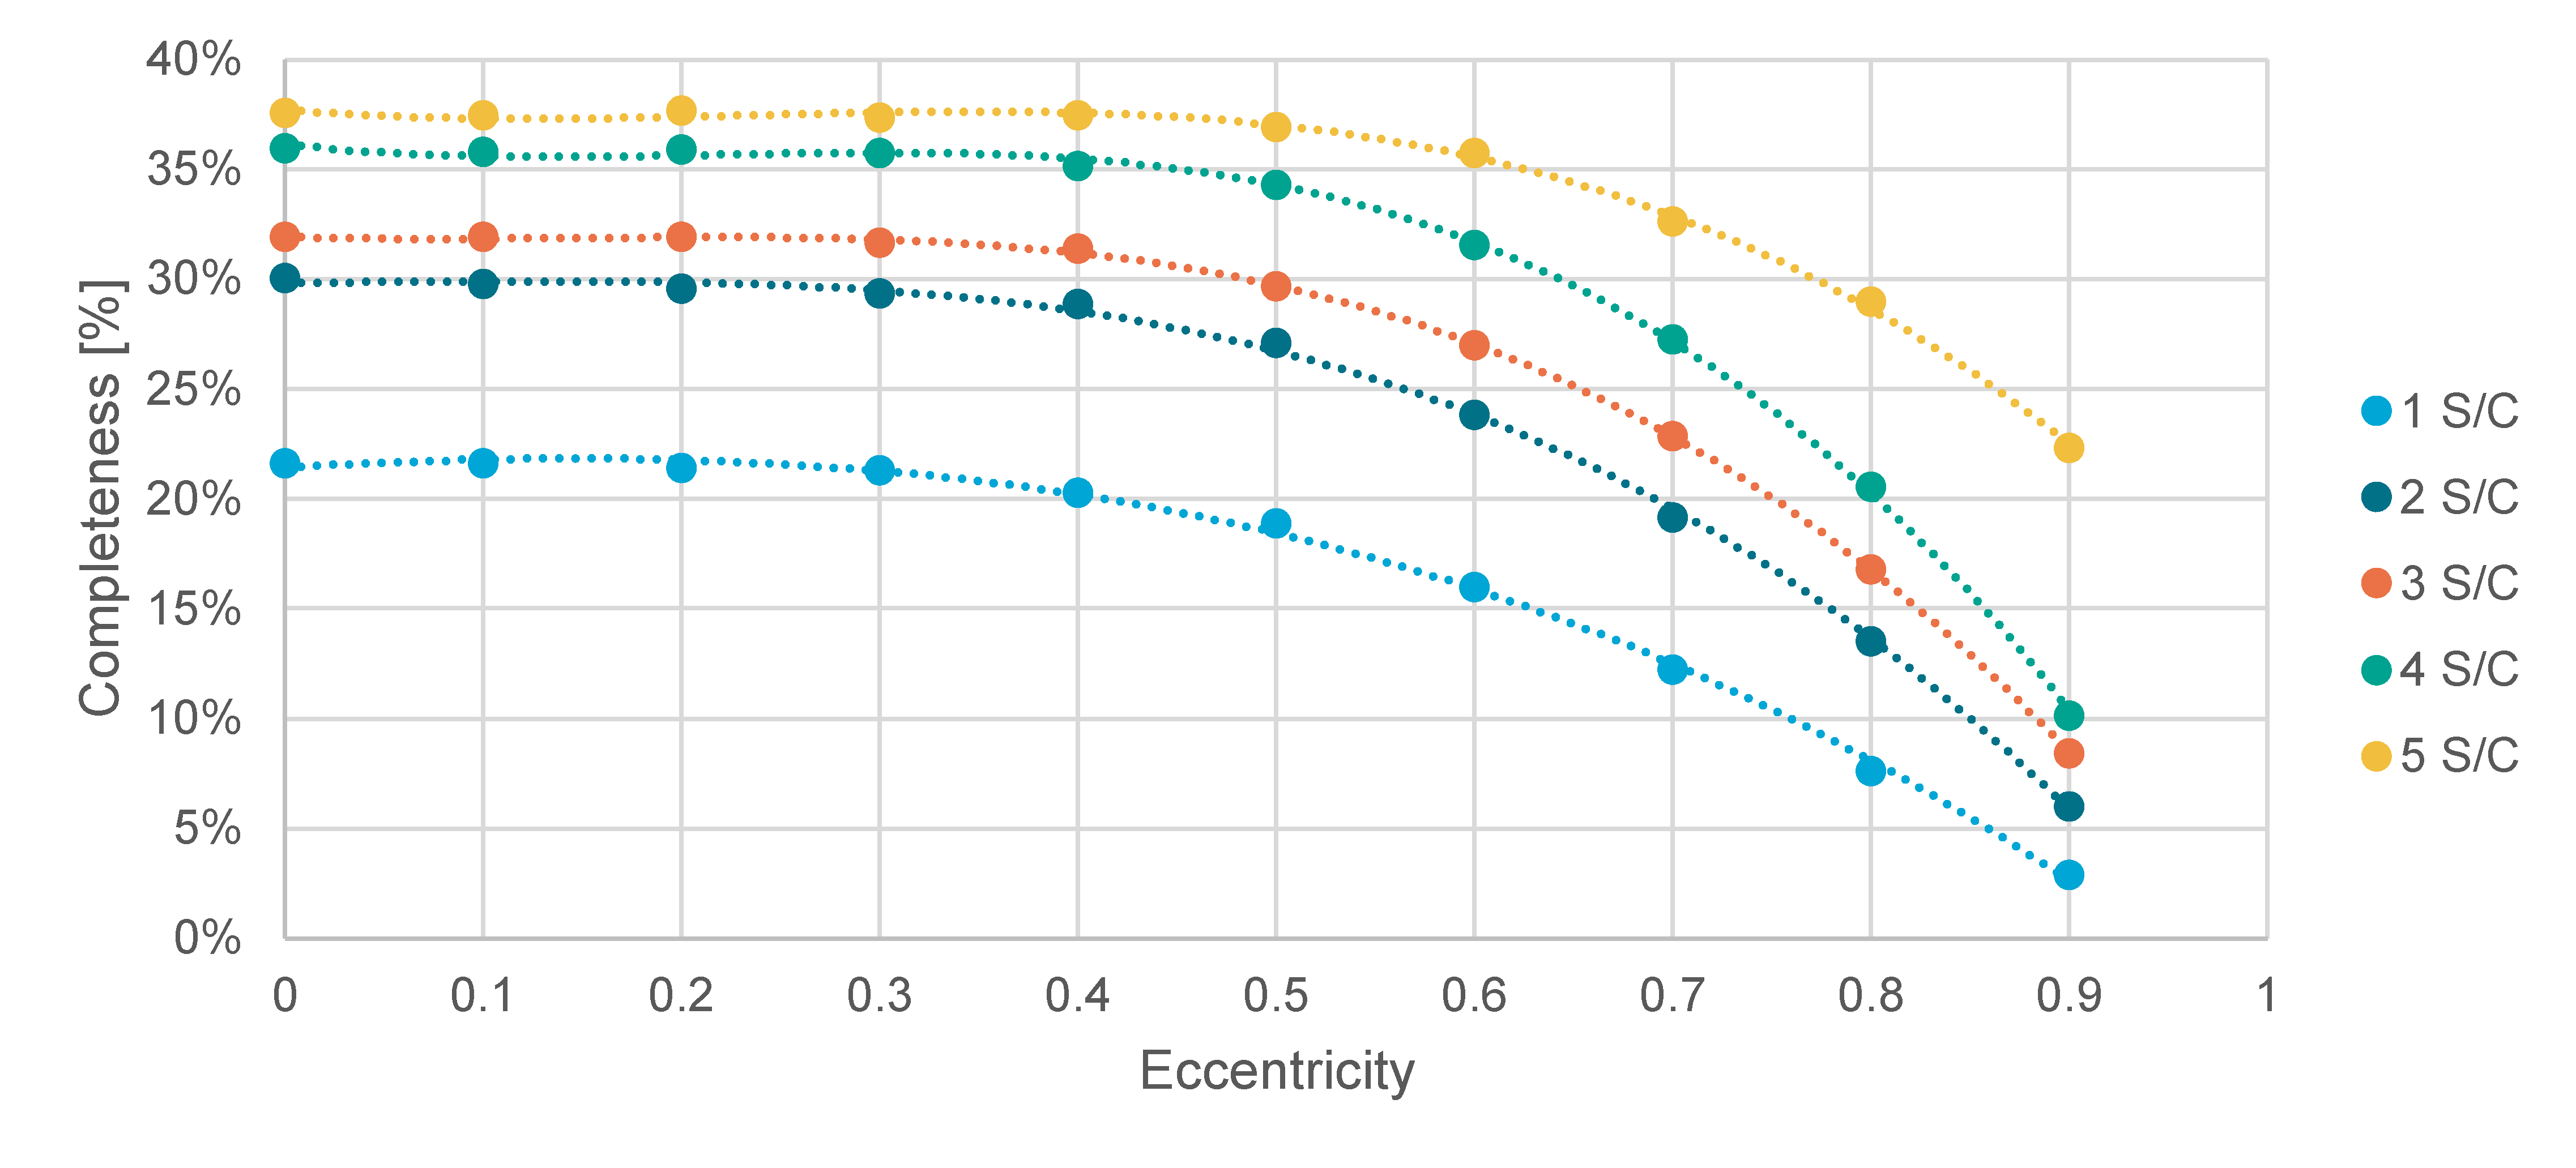
\includegraphics[width=0.8\textwidth]{img/tir_ecc.pdf}
 \caption{Thermal infrared survey performance as a function of eccentricity for 1 to 5 spacecraft. Corresponding semi-major axis and angular separation of spacecraft are optimized using a grid search for each point.}
 \label{fig:tir_ecc}
\end{figure}

Results with regards to varying the eccentricity are shown in \autoref{fig:vis_ecc} for visual light systems and \autoref{fig:tir_ecc} for thermal infrared systems. It is readily apparent that for both systems, a circular orbit is preferred. It is hypothesized that this is the case because eccentricity causes the system to deviate from the optimal semi-major axis found in the previous subsection. This is further supported by the empirical finding that the optimal semi-major axis at a given eccentricity results in an apohelion distance roughly equal to the optimal semi-major axis at 0 eccentricity. That is:
\begin{equation}
 a_{opt}(e) \approx \frac{a_{opt}(0)}{1+e}
\end{equation}
This is further illustrated in \autoref{fig:eccentricity_optimal}. This result is theorized to occur because the spacecraft will, in this solution, still spend a large portion of its orbit in the optimal semi-major axis range. However, not enough data are available to establish statistical significance for this finding.

\begin{figure}[htbp]
 \centering
 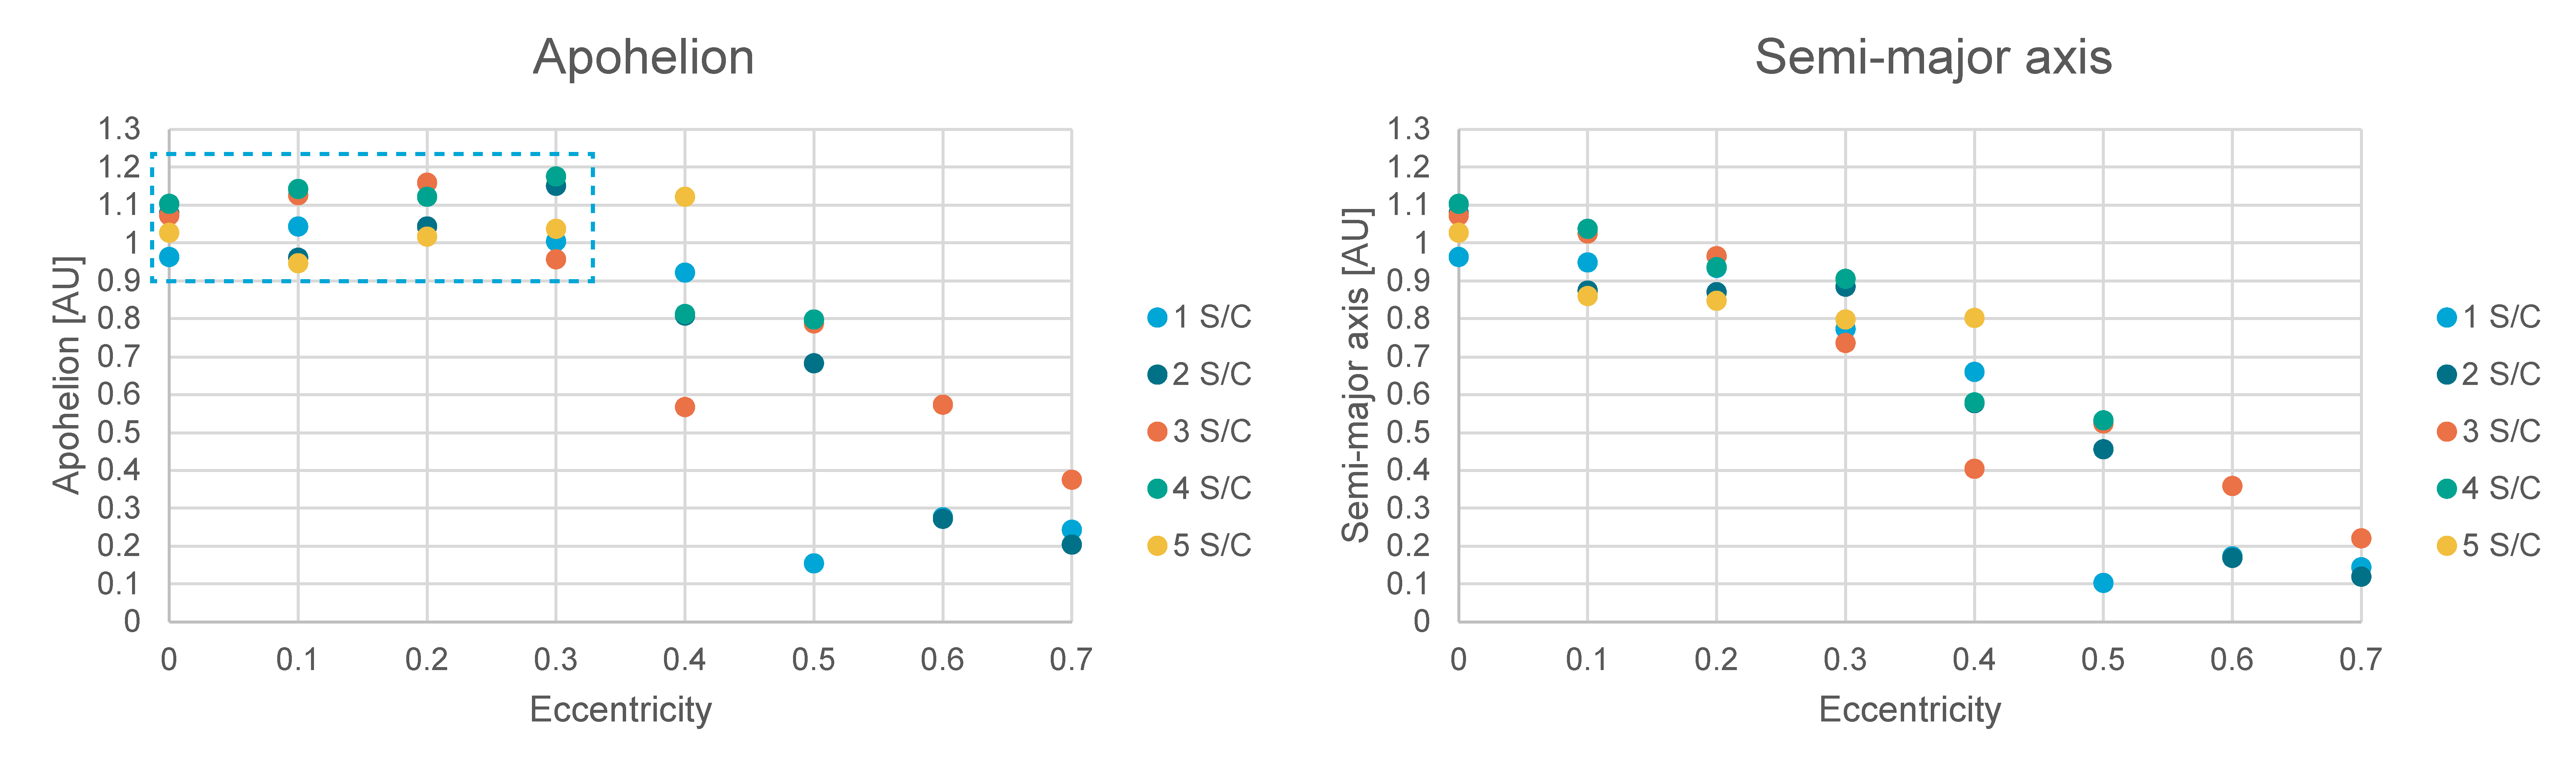
\includegraphics[width=1.0\textwidth]{img/eccentricity_optimal.pdf}
 \caption{Relationship between optimal semi-major axis, eccentricity, and the resulting apohelion for 1-5 spacecraft. It can be seen that the system attempts to maintain the same apohelion for low eccentricities. Corresponding semi-major axis and angular separation of spacecraft are optimized using a grid search for each point.}
 \label{fig:eccentricity_optimal}
\end{figure}


\subsection{Mean Anomaly at Epoch}
\begin{figure}
 \centering
 \includegraphics[width=1.0\textwidth]{img/spread_illustration.png}
 \caption{Illustration of a high ($2\pi/5~\mathrm{rad}$) and a low ($0.3~\mathrm{rad}$) inter-spacecraft distance.}
 \label{fig:spread_illustration}
\end{figure}

The last parameter to be considered for the co-orbital solutions is the mean anomaly at epoch. As previously explained, the mean anomaly will not be considered for each spacecraft separately. Instead, the concept of inter-spacecraft spread is introduced. This inter-spacecraft spread is simply defined as the difference in anomaly at epoch of one spacecraft to the next, in such a way that the formation is centered around $\theta=0$. This means that, with inter-spacecraft spread $\Delta \theta$, the mean anomaly at epoch $\theta$ of spacecraft $n$ in a system of $N$ spacecraft is:
\begin{equation}
 \theta_n = (n-1) \cdot \Delta \theta - \frac{N-1}{2}\Delta \theta
\end{equation}
This equation and the resulting formation is shown in \autoref{fig:spread_illustration}. A lower boundary of 0.3 rad ($\approx 17.2^\circ$) was chosen to ensure triangulation would remain possible. In addition, to maintain the separation between all spacecraft, the full formation can not span more than $2\pi$ rad. This results in the boundaries $0.3 \leq \Delta \theta \leq 2\pi/N$. The hypothesized effect of changing the spread is composed of two effects: On the one hand, spreading out the spacecraft more allows for viewing a larger portion of the sky simultaneously, and reduces blind spots, as explained in \autoref{sec:researchmultispacecraft}. On the other hand, as spacecraft are closer together, the chances of obtaining a simultaneous detection of the same asteroid - and thereby achieving triangulation - is increased, thereby leading to a faster detection.\\

\begin{figure}[htbp]
 \centering
 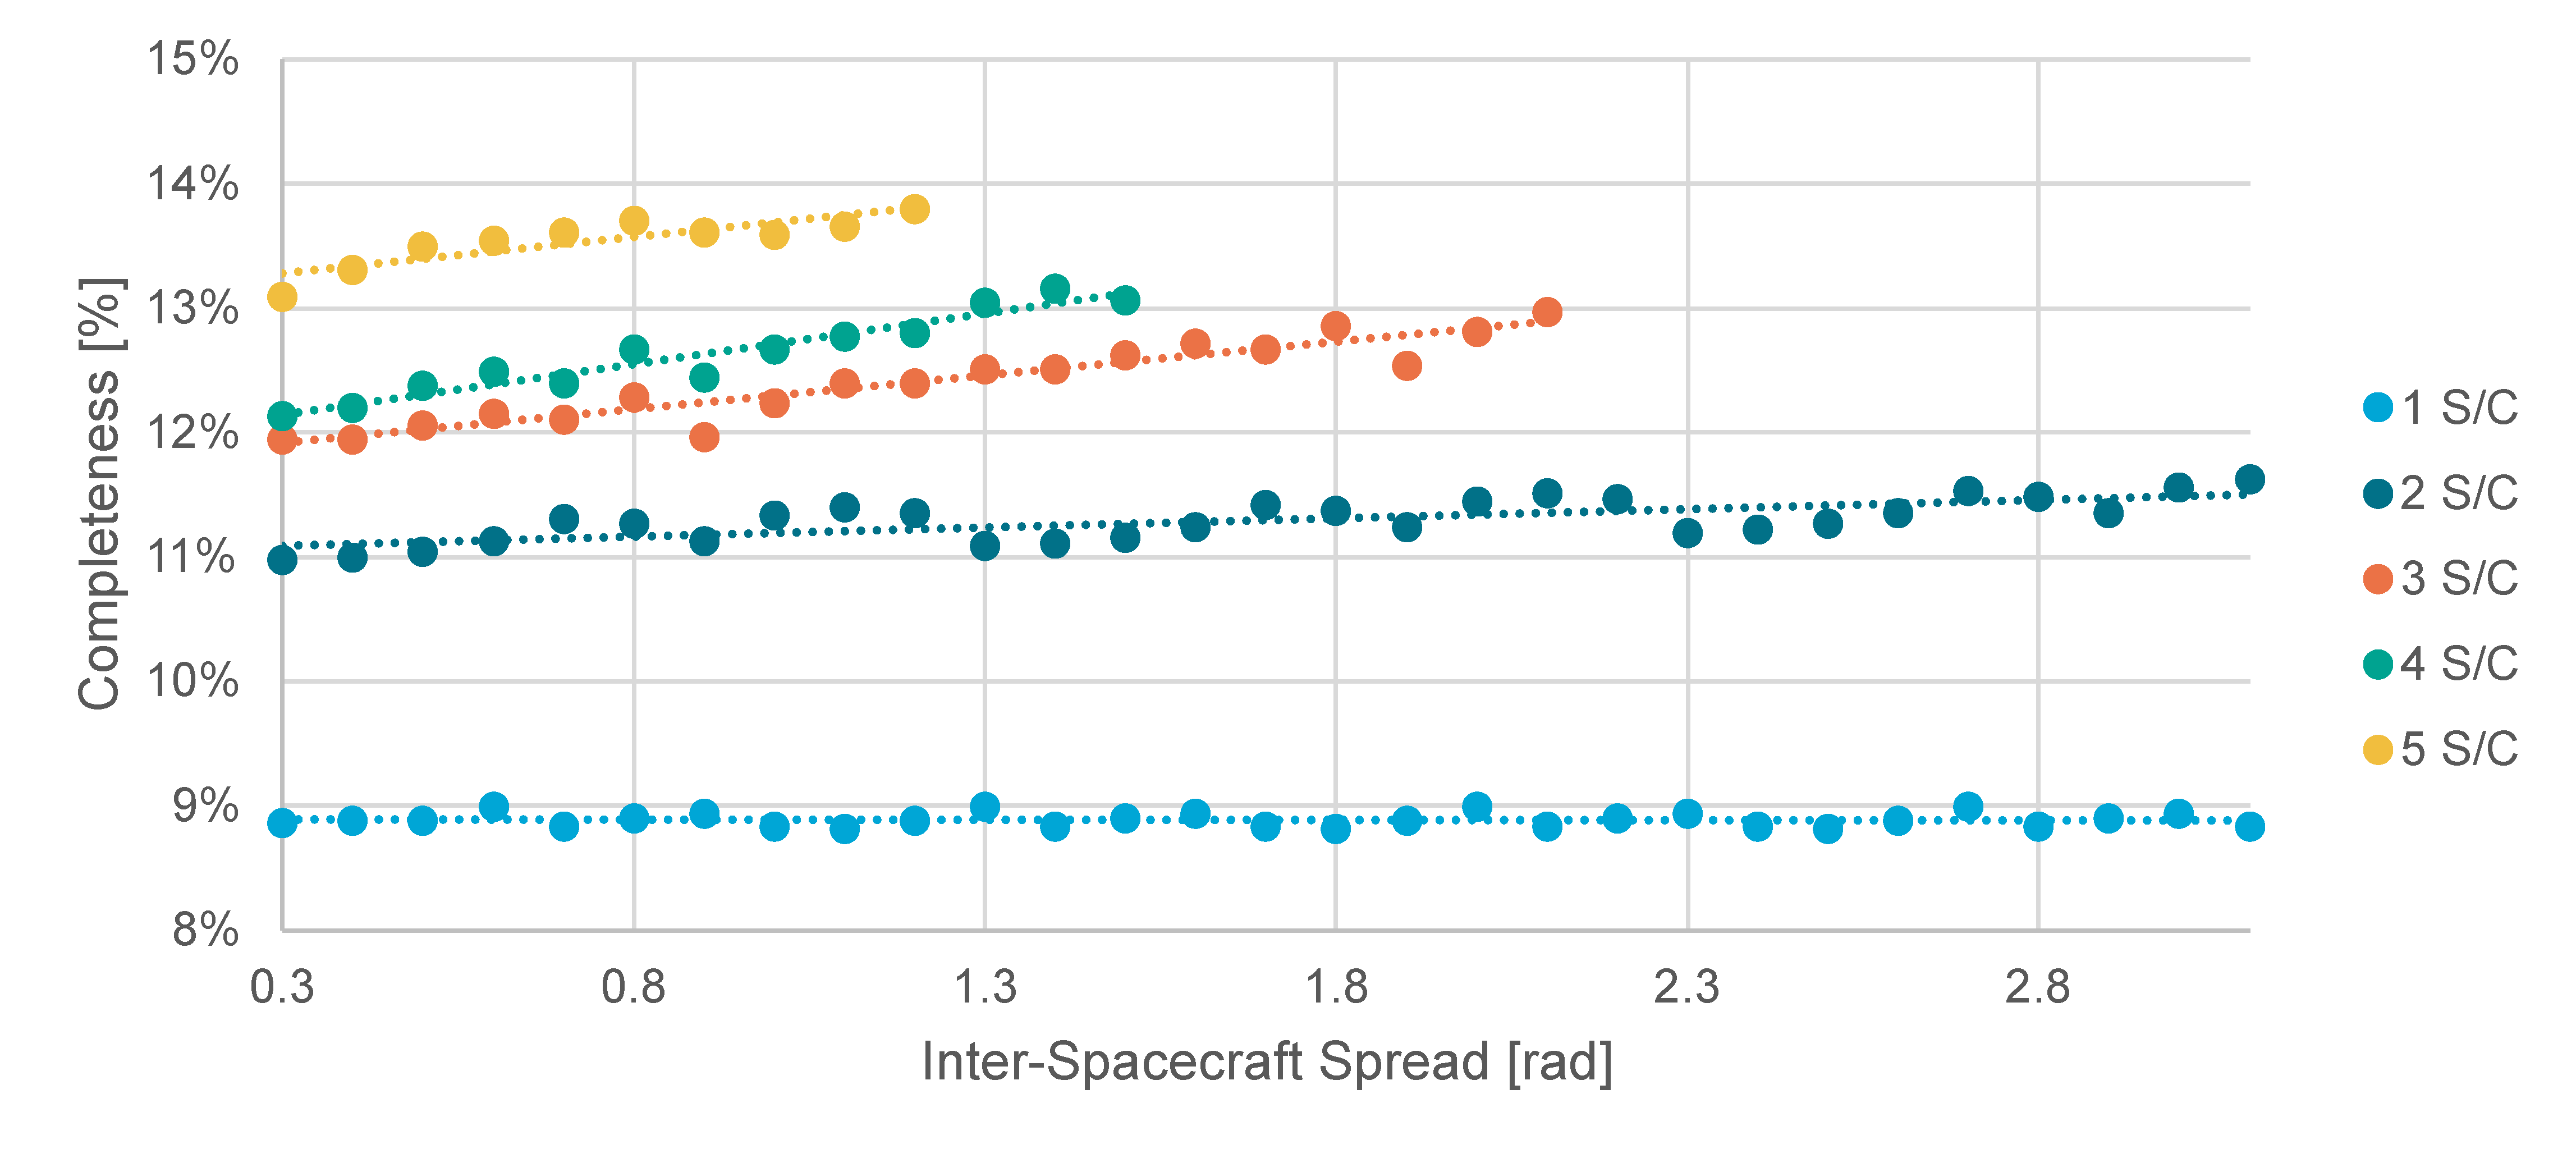
\includegraphics[width=0.8\textwidth]{img/vis_spread.pdf}
 \caption{Visual light survey performance as a function of angular separation between spacecraft for 1 to 5 spacecraft. Corresponding semi-major axis and eccentricity are optimized using a grid search for each point.}
 \label{fig:vis_spread}
\end{figure}

\begin{figure}[htbp]
 \centering
 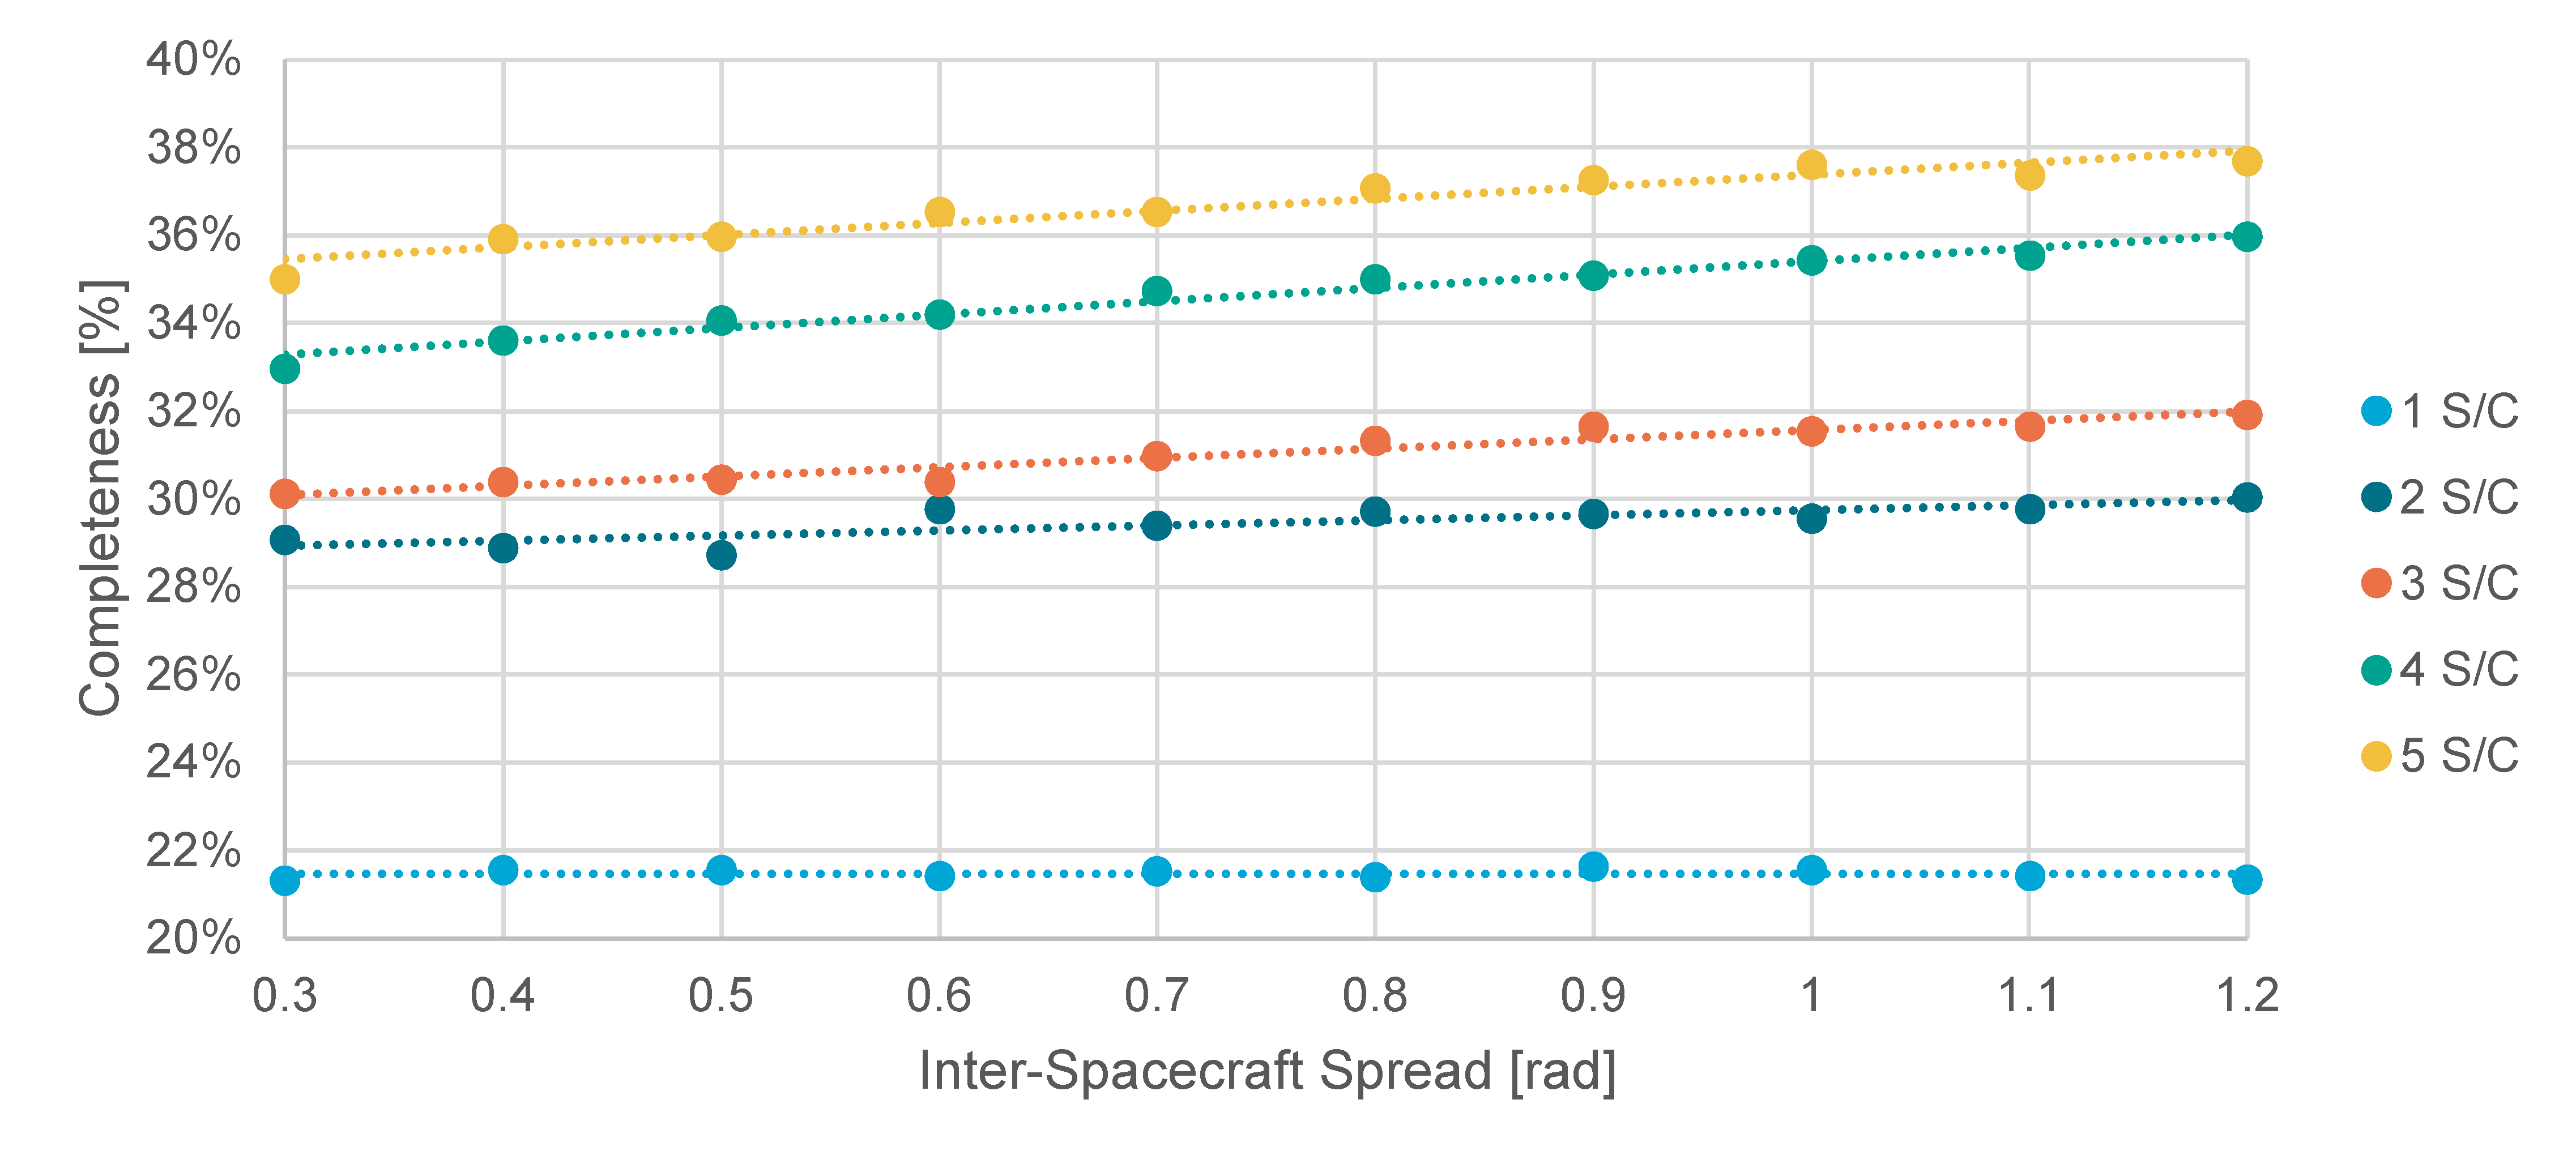
\includegraphics[width=0.8\textwidth]{img/tir_spread.pdf}
 \caption{Thermal infrared survey performance as a function of angular separation between spacecraft for 1 to 5 spacecraft. Corresponding semi-major axis and eccentricity are optimized using a grid search for each point.}
 \label{fig:tir_spread}
\end{figure}

Results for visual light and thermal infrared are shown in \autoref{fig:vis_spread} and \autoref{fig:tir_spread}, respectively. It is observed that an increase in the angular distance between the spacecraft will increase the performance of the system. Therefore, the effect of observing a larger part of the sky effectively is stronger than the increased chance at succesful triangulation. Practically, this implies that a multi-spacecraft survey should aim to distribute the spacecraft as much as possible over the orbit, even if e.g. communications requirements do not allow the system to be spread out over the entire orbit. In the next section, a hypothesis will be developed to explain the observed phenomena, and provide a basis for the prediction of the performance of the non-co-orbital systems to be considered later.

\section{Number of Spacecraft}
\label{sec:results_number}

\begin{figure}[htbp]
 \centering
 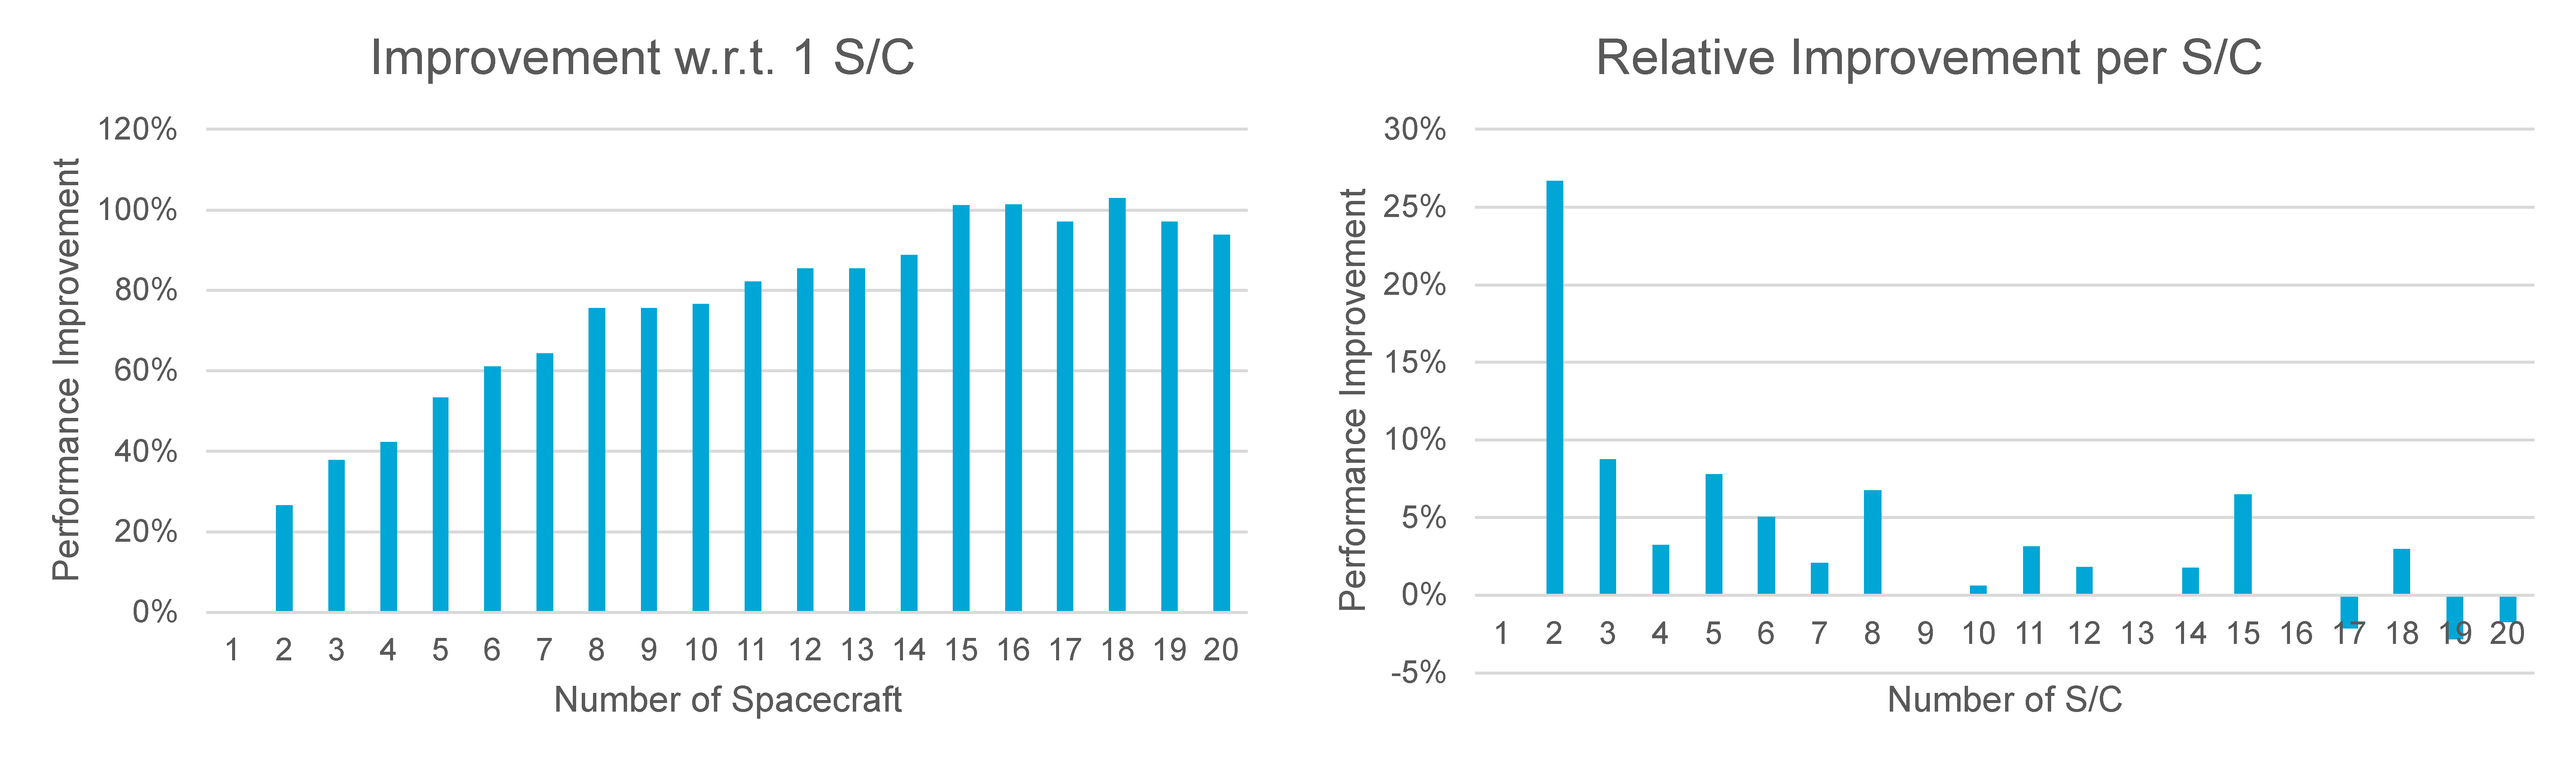
\includegraphics[width=1.0\textwidth]{img/number_sc_vis.pdf}
 \caption{Improvement in survey completeness gained by increasing the number of spacecraft in a purely visual light wavelength system, including standard deviation bars (from 10 iterations). The left graph shows the improvement of an $n$-spacecraft system with respect to a system of a single spacecraft, the right graph shows the improvement of an $n$-spacecraft system with respect to an $n-1$-spacecraft system.}
 \label{fig:results_number_vis}
\end{figure}


\begin{figure}[htbp]
 \centering
 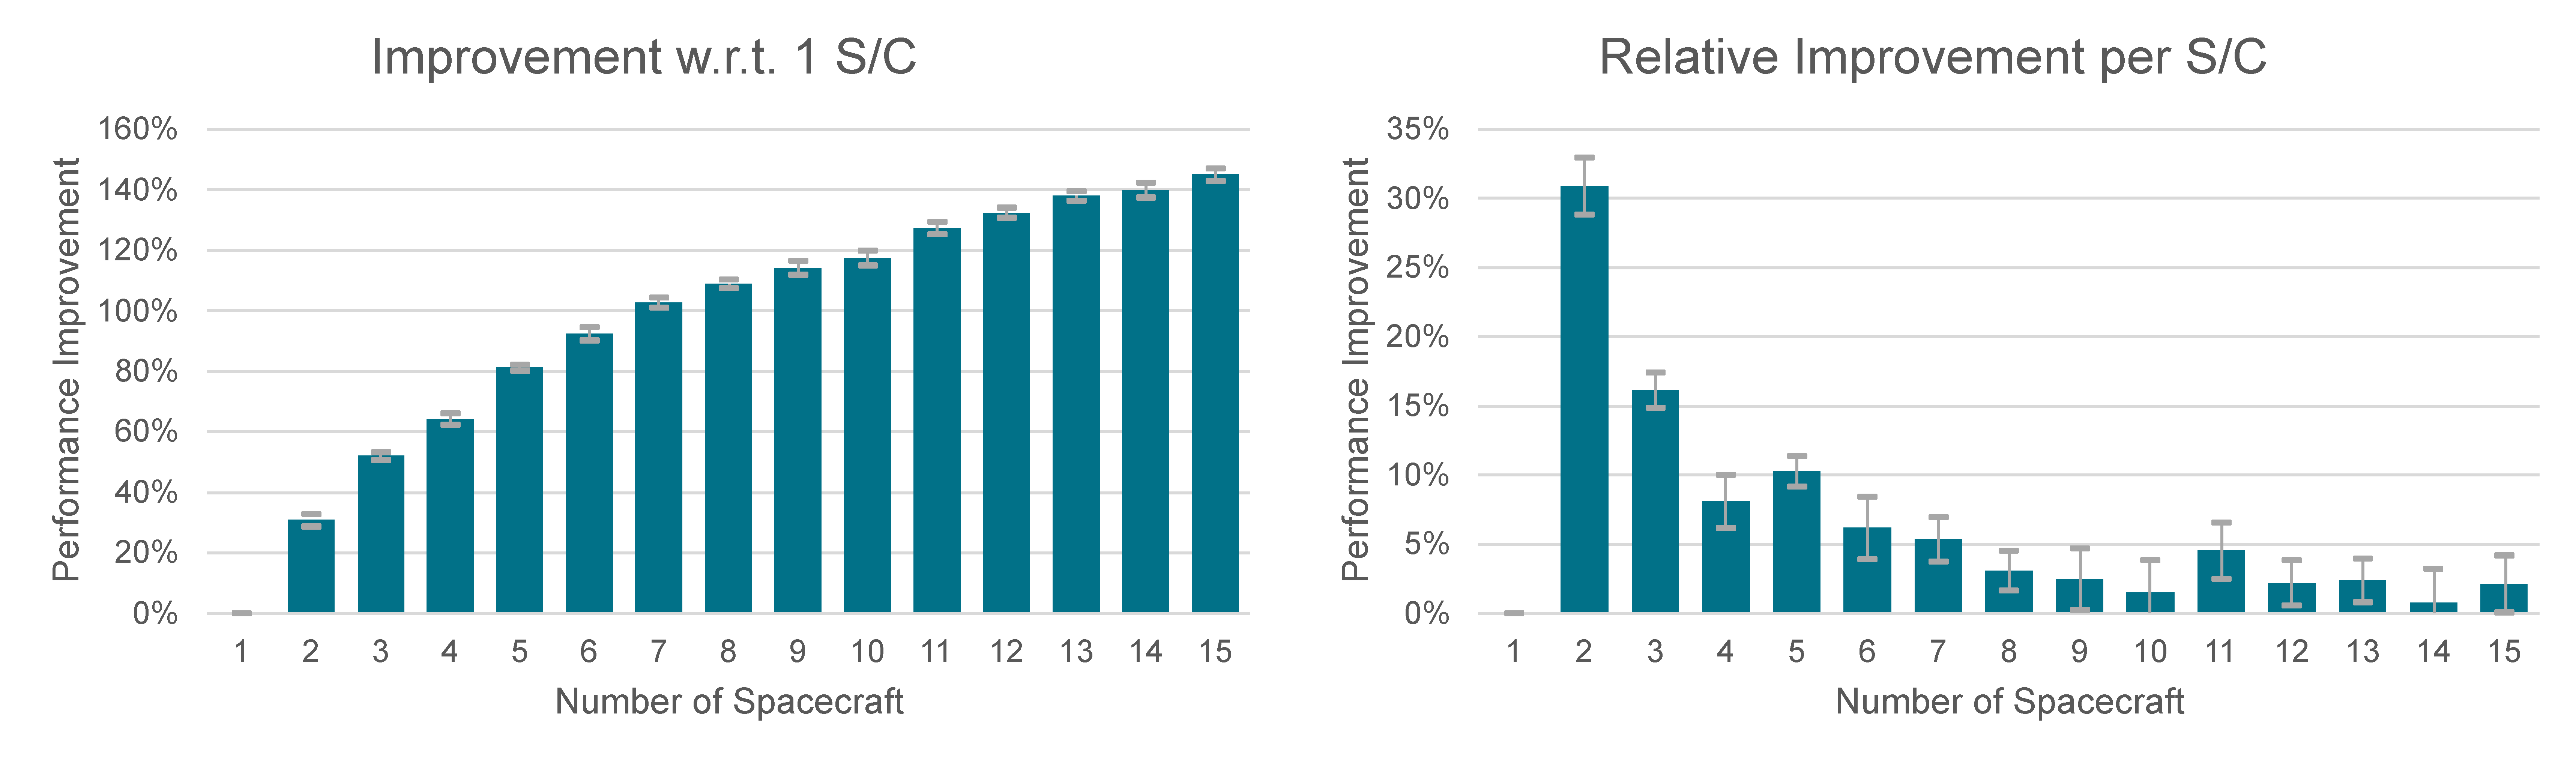
\includegraphics[width=1.0\textwidth]{img/number_sc_tir.pdf}
 \caption{Improvement in survey completeness gained by increasing the number of spacecraft in a purely thermal infrared wavelength system, including standard deviation bars (from 10 iterations). The left graph shows the improvement of an $n$-spacecraft system with respect to a system of a single spacecraft, the right graph shows the improvement of an $n$-spacecraft system with respect to an $n-1$-spacecraft system.}
 \label{fig:results_number_tir}
\end{figure}

As explained previously, the number of spacecraft in the system is a parameter that does not have an optimum with respect to the obtained survey completeness: adding additional spacecraft will logically never degrade the performance of the system. However, in practice other constraints (primarily economical) will be present. Therefore, the increase in performance resulting from such an increased investment is of particular interest. \autoref{fig:results_number_vis} and \autoref{fig:results_number_tir} show the performance increase obtained as a function of the number of spacecraft, for the visual spectrum and thermal infrared, respectively. All results were obtained using the optimal orbital elements deduced in the previous section. Several observations can be made, which will be listed and subsequently discussed below.\\

Firstly, significant diminishing returns present themselves for both spectra; the additional value of an extra spacecraft decreases exponentially with the number of spacecraft already present in the system. Performance increases gained per additional spacecraft fall to around 5\% when surpassing 5 spacecraft in the system. Beyond 10 spacecraft, the increases start to become smaller than the standard deviation in the results. This means that, although large initial improvements in performance can be gained from utilizing a multi-spacecraft system, simply increasing the number of survey spacecraft can not bring us arbitrarily close to 100\% survey completeness; when increasing beyond approximately 5 spacecraft, it is recommended to focus efforts on improving other areas of the system for the mission to remain efficient. \\

This fact compounds the second finding: even the most efficient addition - adding a second spacecraft to a single spacecraft survey system - does not come close to increasing the system performance by 100\%. In other words: increasing the number of spacecraft will \textit{decrease} the number of asteroids detected \textit{per spacecraft}. While this finding might seem irrelevant from a mission design point-of-view - the overall performance still increases - it is nevertheless important to consider in the context of other mission constraints, such as budget. \\

The third result is that thermal infrared systems feature a larger relative improvement to survey performance as the number of spacecraft increases, i.e. thermal infrared systems benefit more from additional spacecraft. This trend continues for higher numbers of spacecraft, with thermal infrared systems reaching a 100\% improvement around 7-8 spacecraft, compared to visual light systems requiring 15-16 spacecraft to achieve a similar performance gain. This, combined with the fact that thermal infrared systems have been shown to be the best choice for future NEA missions using a single spacecraft (see e.g. \cite{2017NEOSDT}, \cite{ThesisOlga}), suggests a multi-spacecraft system should also comprise thermal infrared telescopes. This will be investigated in more detail in \autoref{sec:results_payload}.\\

Finally, it is evident that a variance of around 1-2\% is present in the survey performance results, relative to a smooth exponentially decreasing curve. It was found that this variance is also present when repeatedly sampling the simulation using the same input parameters. Therfore, in these and subsequent results, it will be assumed that this is simply a result of the stochasticity in the model. Possible other explanations will be ruled out further in \autoref{ch:vandv}.

\section{Payload}
\label{sec:results_payload}
\begin{figure}[htbp]
 \centering
 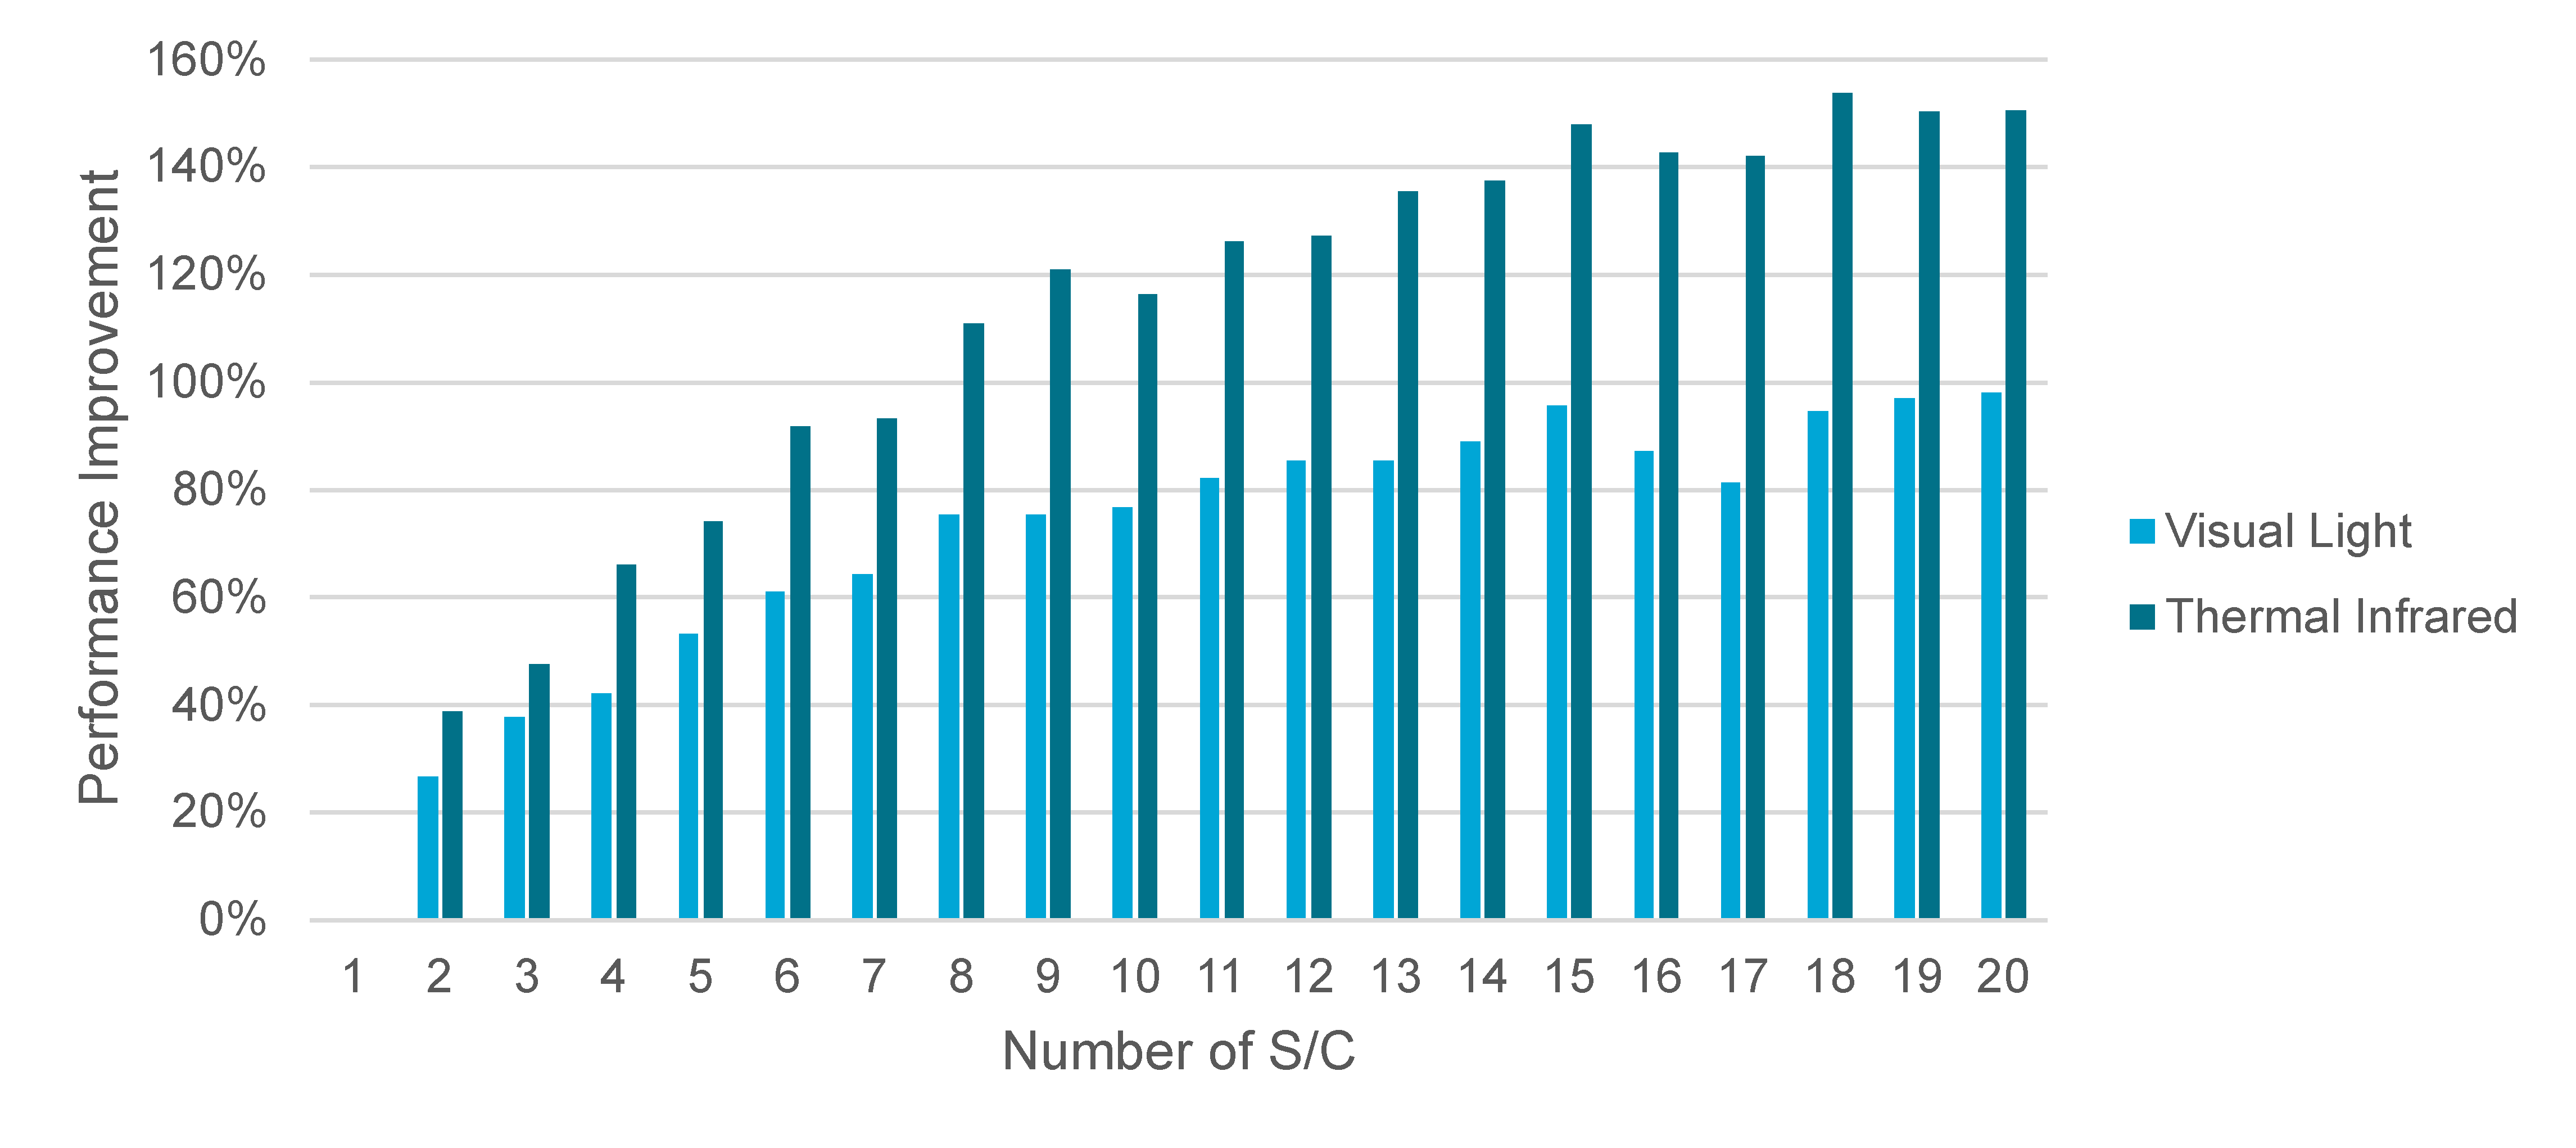
\includegraphics[width=0.8\textwidth]{img/tir_vs_vis_many.pdf}
 \caption{Comparison of relative increase in performance gained relative to a single spacecraft system for visual and thermal infrared systems.}
 \label{fig:tir_vs_vis_many}
\end{figure}

\begin{figure}[htbp]
 \centering
 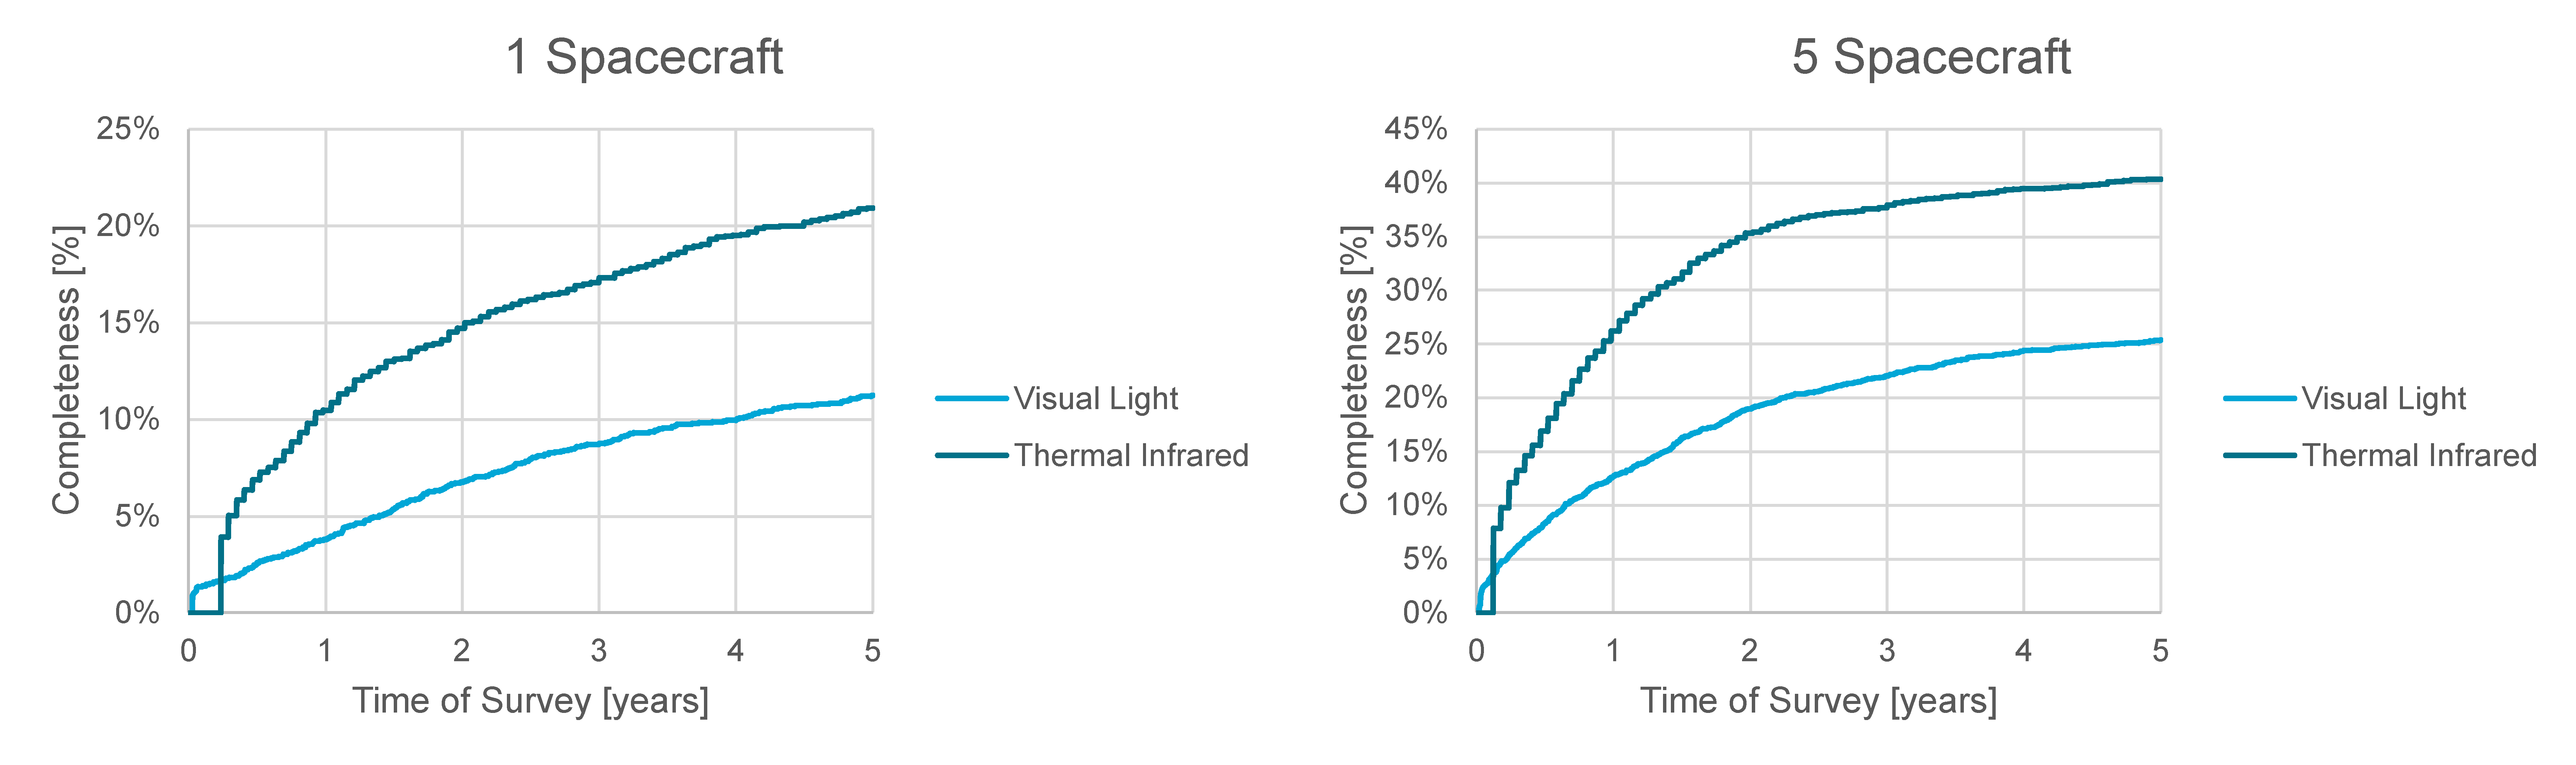
\includegraphics[width=1.0\textwidth]{img/tir_vs_vis_1_5.pdf}
 \caption{Progress of survey completeness over a five year survey for a 1-spacecraft and 5-spacecraft system, in systems where either all spacecraft are equipped with visual light telescopes, or all spacecraft are equipped with thermal infrared telescopes.}
 \label{fig:tir_vs_vis_nohybrid}
\end{figure}


As mentioned in the previous section, initial result suggest thermal infrared systems to be the optimal choice for multi-spacecraft systems because of their predicted higher performance in single-spacecraft systems, and higher benefit from increasing the number of spacecraft. The latter effect is shown in \autoref{fig:tir_vs_vis_many}. In this section, the payload composition will be investigated in more detail. Particular interest is placed in the performance as a function of time - visual light systems feature a faster cadence - and in possible synergistic effects in systems featuring both visual light and thermal infrared telescopes. When interpreting the results of this chapter, it is important to keep in mind the fact that these simulations were carried out assuming contemporary hardware (as listed in \autoref{tab:hardwareproperties}). Advances in either type of telescope or sensor might warrant a future reassessment.\\

Firstly, the performances for systems featuring only one payload type were modelled. For comparison, this analysis was carried out for a 1-spacecraft and a 5-spacecraft system. Because, as shown in the previous section, the payload types exhibit similar behavior when the number of spacecraft is altered, this was assumed to be representative of other numbers of spacecraft as well. The resulting survey performance as a function of time can be seen in \autoref{fig:tir_vs_vis_nohybrid}. Note that, contrary to previous figures, these graphs show the \textit{absolute} survey completeness, not the completeness relative to a benchmark. In the results, it can be observed that initially, the visual light system features a higher completeness due to its faster cadence. However, the thermal infrared system quickly surpasses it as time progresses. This means that the faster cadence granted by the lower integration times and larger sensor sizes of the visual light system does not weigh up to the increased sensitivity of the thermal infrared system on the timescales of survey missions; not only is the final survey completeness more than 10\% higher for a thermal infrared system, it also manages to achieve the same performance as a 5-year visual light survey in only a single year in both examined cases. This agrees with the findings of \cite{ThesisOlga} that for systems where quick detections are important, such as impact last-warning, thermal infrared is also a superior option. \\

\begin{figure}[htbp]
 \centering
 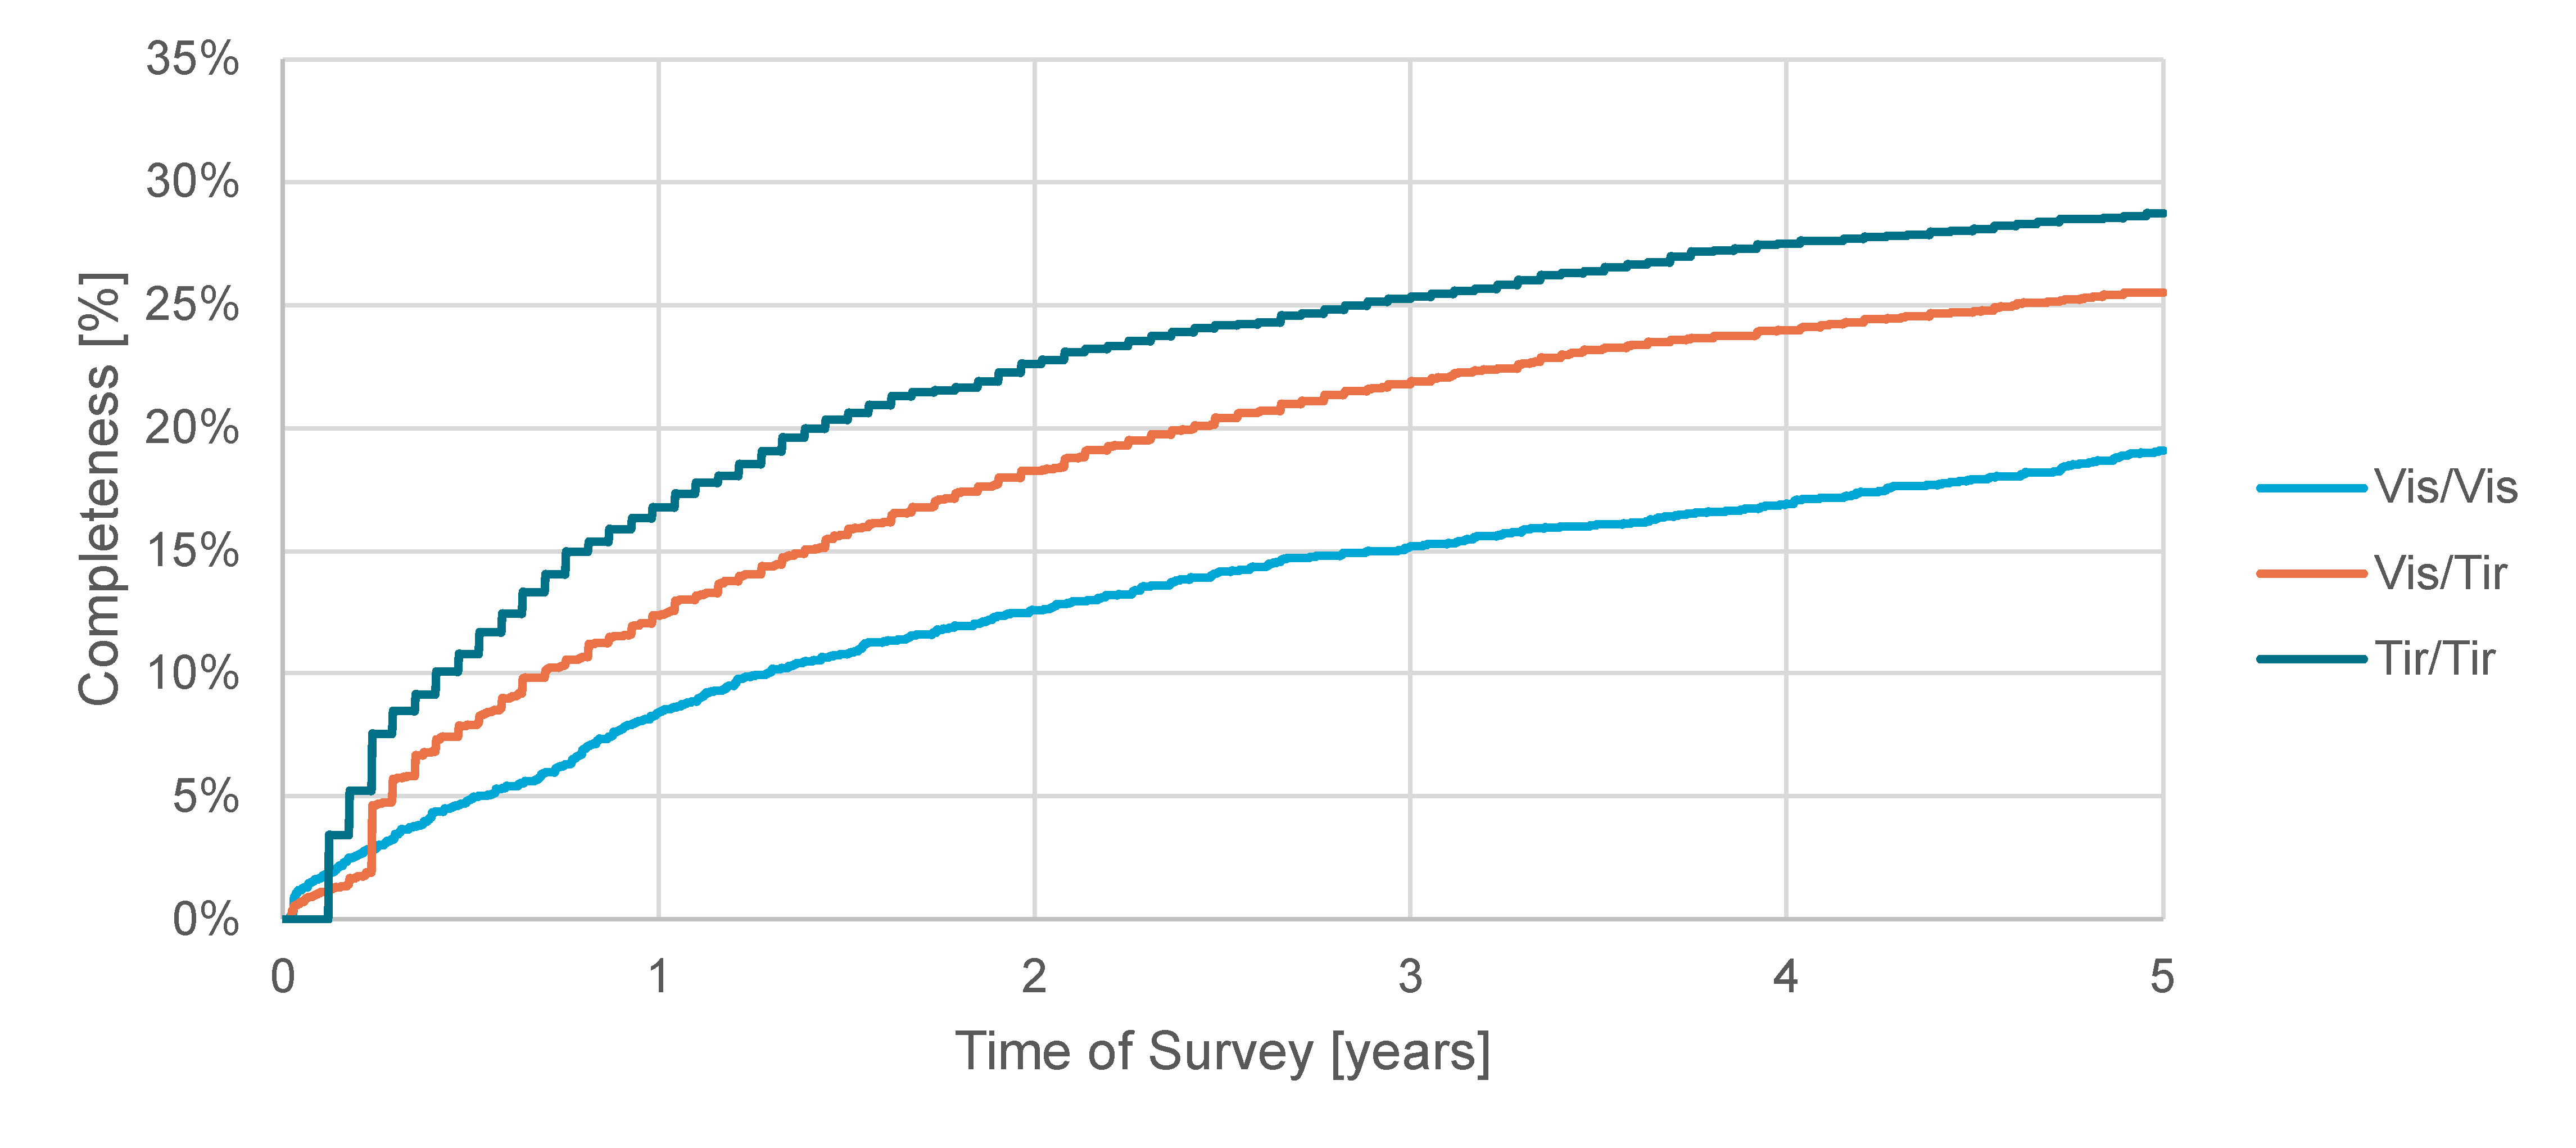
\includegraphics[width=0.8\textwidth]{img/tir_vs_vis_2_hybrid.pdf}
 \caption{Progress of survey completeness over a five year survey for all possible payload combinations in a 2-spacecraft system.}
 \label{fig:payload_hybrid_one}
\end{figure}

\begin{figure}[htbp]
 \centering
 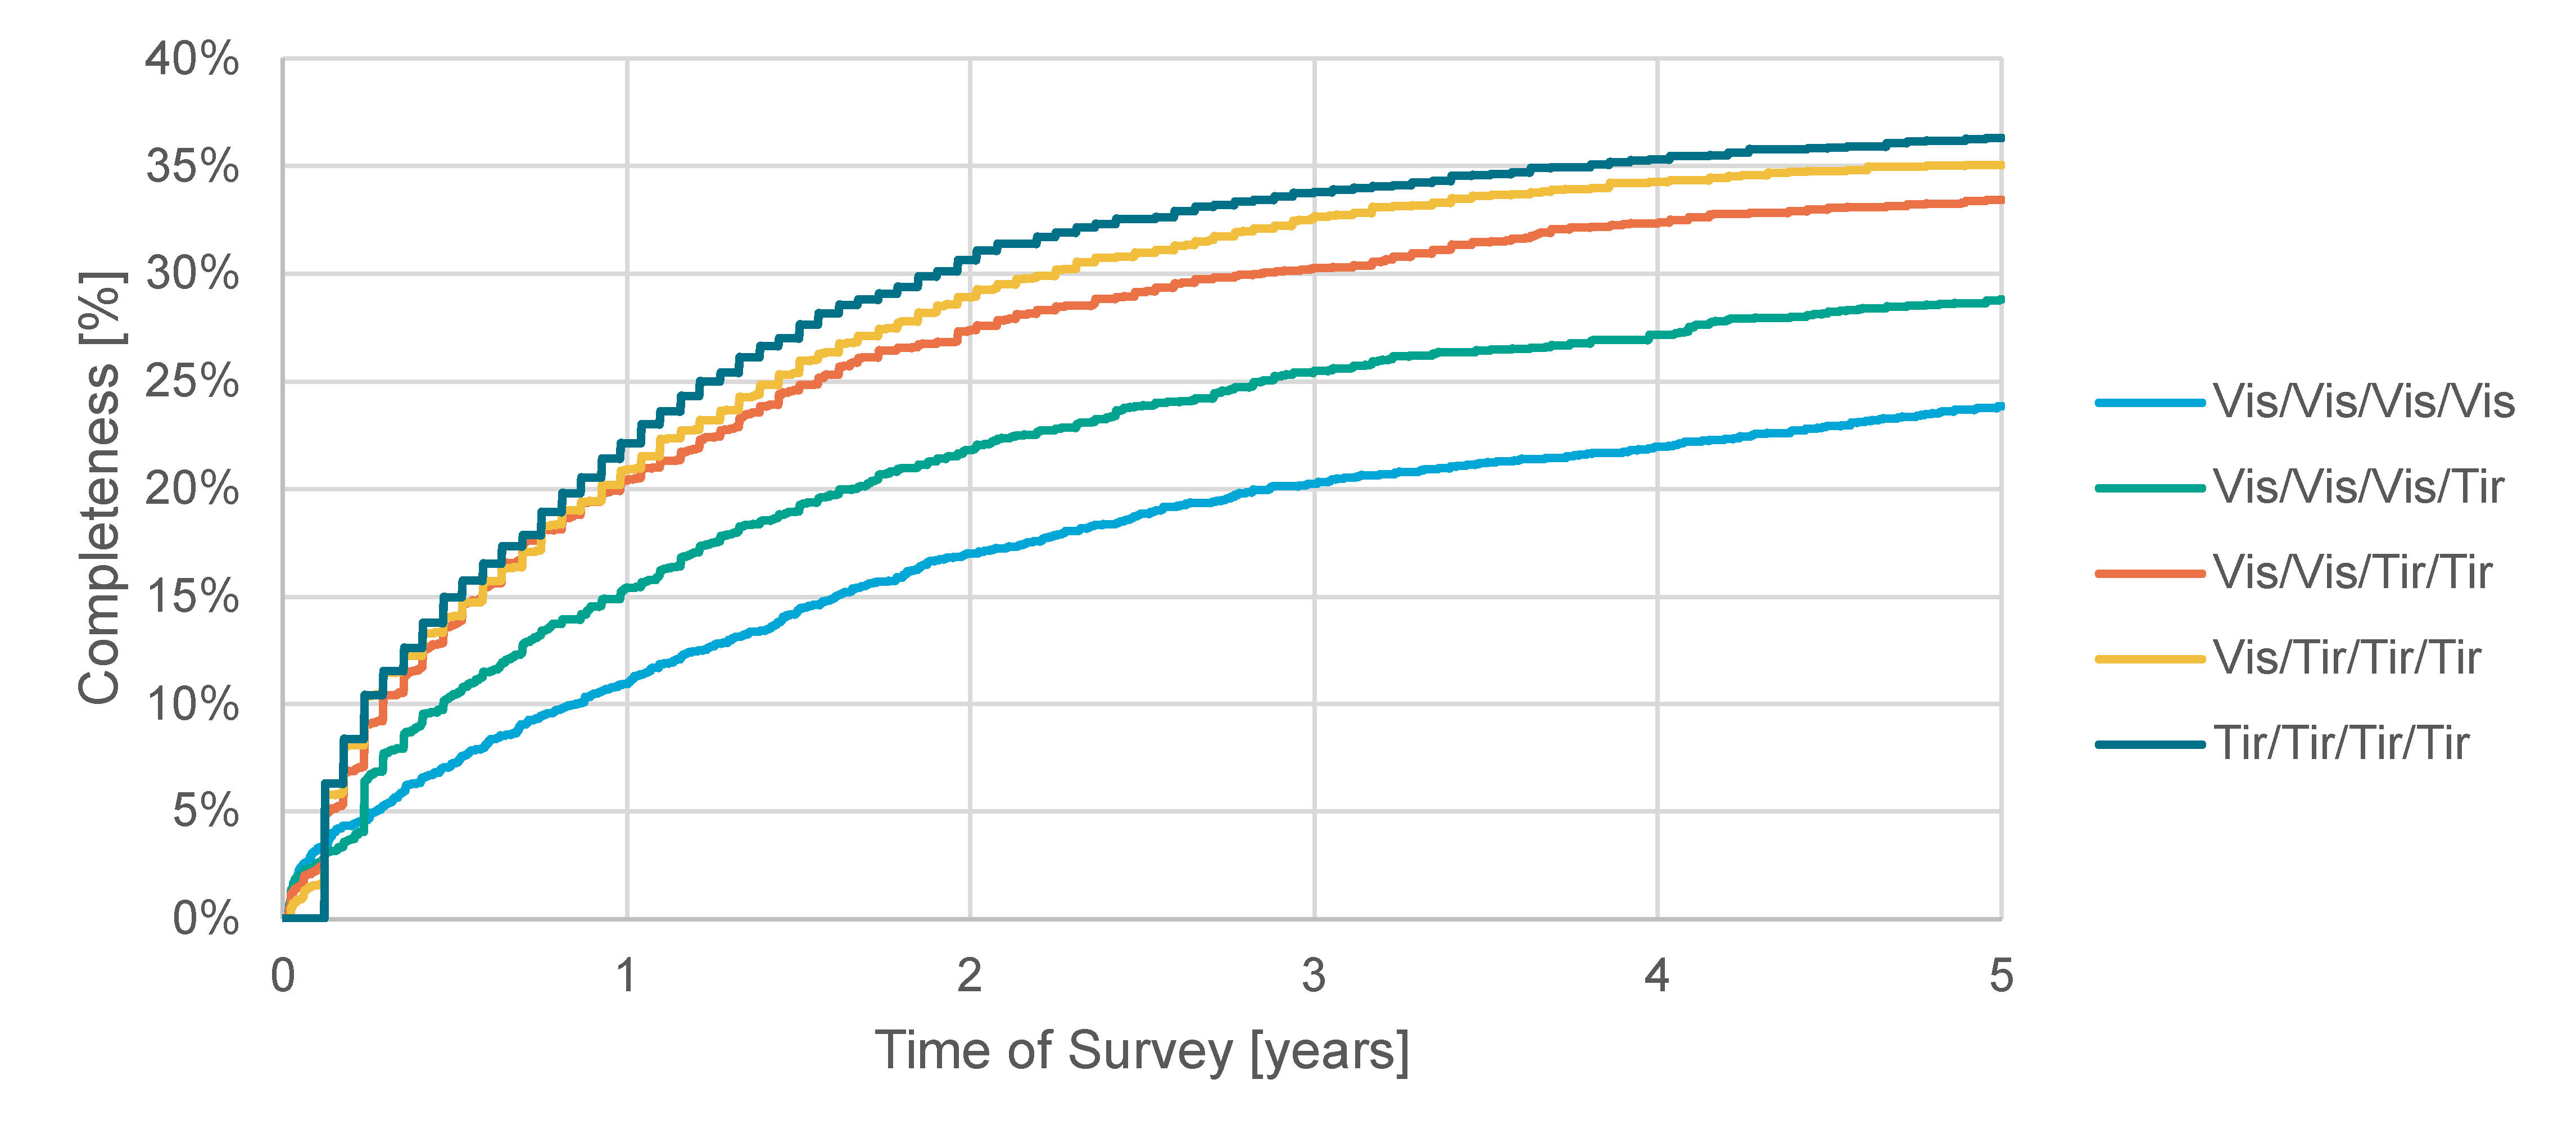
\includegraphics[width=0.8\textwidth]{img/tir_vs_vis_4_hybrid.pdf}
 \caption{Progress of survey completeness over a five year survey for all possible payload combinations in a 4-spacecraft system.}
 \label{fig:payload_hybrid_two}
\end{figure}

In continuation of the payload analysis, systems utilizing a combination of visual light and thermal infrared telescopes were examined. The reasoning is that the higher sensitivity of thermal infrared systems combined with the higher cadence of visual light systems might result in a synergistic effect where the system performs better than the performance of the individual components would suggest. However, as can be seen from the results for 2- and 4-spacecraft systems in \autoref{fig:payload_hybrid_one} and \autoref{fig:payload_hybrid_two}, respectively, this is not the case. A system comprising purely infrared telescopes yields the best results, and performance increases progressively as the number of thermal infrared telescopes in the system increases. This means that in general thermal infrared is the preferred payload type for deep space multi-spacecraft systems aimed at increasing the survey completeness. Note however that this assertion is made under the assumption of a simplistic search strategy, where the system repeatedly images the entire sky. Possible applications of fast visual light telescopes as follow-up telescopes - as demonstrated by the Catalina Sky Survey - might still be a feasible option, although this would first require research into such advanced search strategies.



\section{Explanation of Observed Phenomena}
\label{sec:results_explanation}
To complement and support the previously obtained results, in this section an explanation is proposed to the observed phenomena. Specifically, an attempt will be made to explain the performance increase gained by spreading the spacecraft apart, the increase in optimal semi-major axis as a function of number of spacecraft, and the fact that eccentric orbits yield worse results. In addition, an hypothesis will be drafted for the performance of the non-co-orbital systems, which are analysed in the next section. \\

The proposed mechanism which drives the witnessed performance is through the volume of space which can be covered by the telescope. In other words: A system which can obtain a good SNR on targets in a larger volume of space will outperform a system which has a smaller area where that SNR can be achieved. Simulations were performed on the ecliptic plane, from -5 to +5 AU in both directions, and the limiting magnitude required to achieve an SNR $\geq$ 5 was determined for each point on the plane. \autoref{fig:coverageexplanation} shows an example calculation, with annotation to aid in understanding the illustration. Next to the Sun, spacecraft, and the spacecraft's orbit, the graph shows \textit{the limiting absolute magnitude} (i.e., the smallest NEA) which can be detected at SNR $\geq$ 5 at a specified location.\\

\begin{figure}[htbp]
 \centering
 \includegraphics[width=0.8\textwidth]{img/coverage_explanation_text.png}
 \caption{Explanation of the resulting diagram of coverage area. The color of the area indicates the limiting absolute magnitude of NEA which can still be successfully detected in a given area. Also shown are the Sun, spacecraft, and the orbit of the spacecraft. Several expected phenomena are indicated in the image. Coordinates in the $e$ frame, viewing in the negative $Z_e$-direction.}
 \label{fig:coverageexplanation}
\end{figure}


\begin{figure}[htbp]
 \centering
 \includegraphics[width=1.0\textwidth]{img/coverage_spread.png}
 \caption{Illustration of the observable area for a system of 1, 3 and 5 spacecraft, spread out over the orbit. Coordinates in the $e$ frame, viewing in the negative $Z_e$-direction.}
 \label{fig:coverage_spread}
\end{figure}

In \autoref{fig:coverage_spread} the results of this simulation can be seen for 1, 2 and 5 spacecraft in a 1 AU circular orbit, spread out equally. Several things should be noted about the results here before continuing: Firstly, it can be seen that increasing the number of spacecraft allows for covering the ``blind spots'' caused by Solar glare already at low numbers of spacecraft. The blind area in line with the Sun which can be seen in the diagram with only a single spacecraft is almost completely covered by three spacecraft. Secondly, already at low numbers of spacecraft, a large area is covered at low absolute magnitude (i.e., large asteroids). Lastly, asteroids with a high absolute magnitude (i.e., small asteroids) can only be detected very close to a spacecraft. \\

\begin{figure}[htbp]
 \centering
 \includegraphics[width=1.0\textwidth]{img/coverage_tight.png}
 \caption{Illustration of the observable area for a system of 1, 3 and 5 spacecraft, spread apart by 0.2 rad ($\approx 11.5^\circ$). Coordinates in the $e$ frame, viewing in the negative $Z_e$-direction.}
 \label{fig:coverage_tight}
\end{figure}


The findings here can be constrasted with the results obtained when the spacecraft are not spread out, as can be seen in \autoref{fig:coverage_tight}. Three things here are noted: the reduction in blind spots is less effective, still leaving a large area obstructed by the Sun. Secondly, the system is no longer capable of detecting large asteroids in almost the entire search volume. The actual size of the ``bubble'' grows only marginally with additional spacecraft. Lastly, even for the areas where small NEAs can be detected, some overlap is present which will also decrease the performance. Therefore, the actual volume where NEAs can be effectively detected is decreased by a sizeable amount when not spreading apart the spacecraft, and the performance gains are instead only caused by an increase in the number of times the sky is imaged (effectively speeding up the cadence).\\

\begin{figure}[htbp]
 \centering
 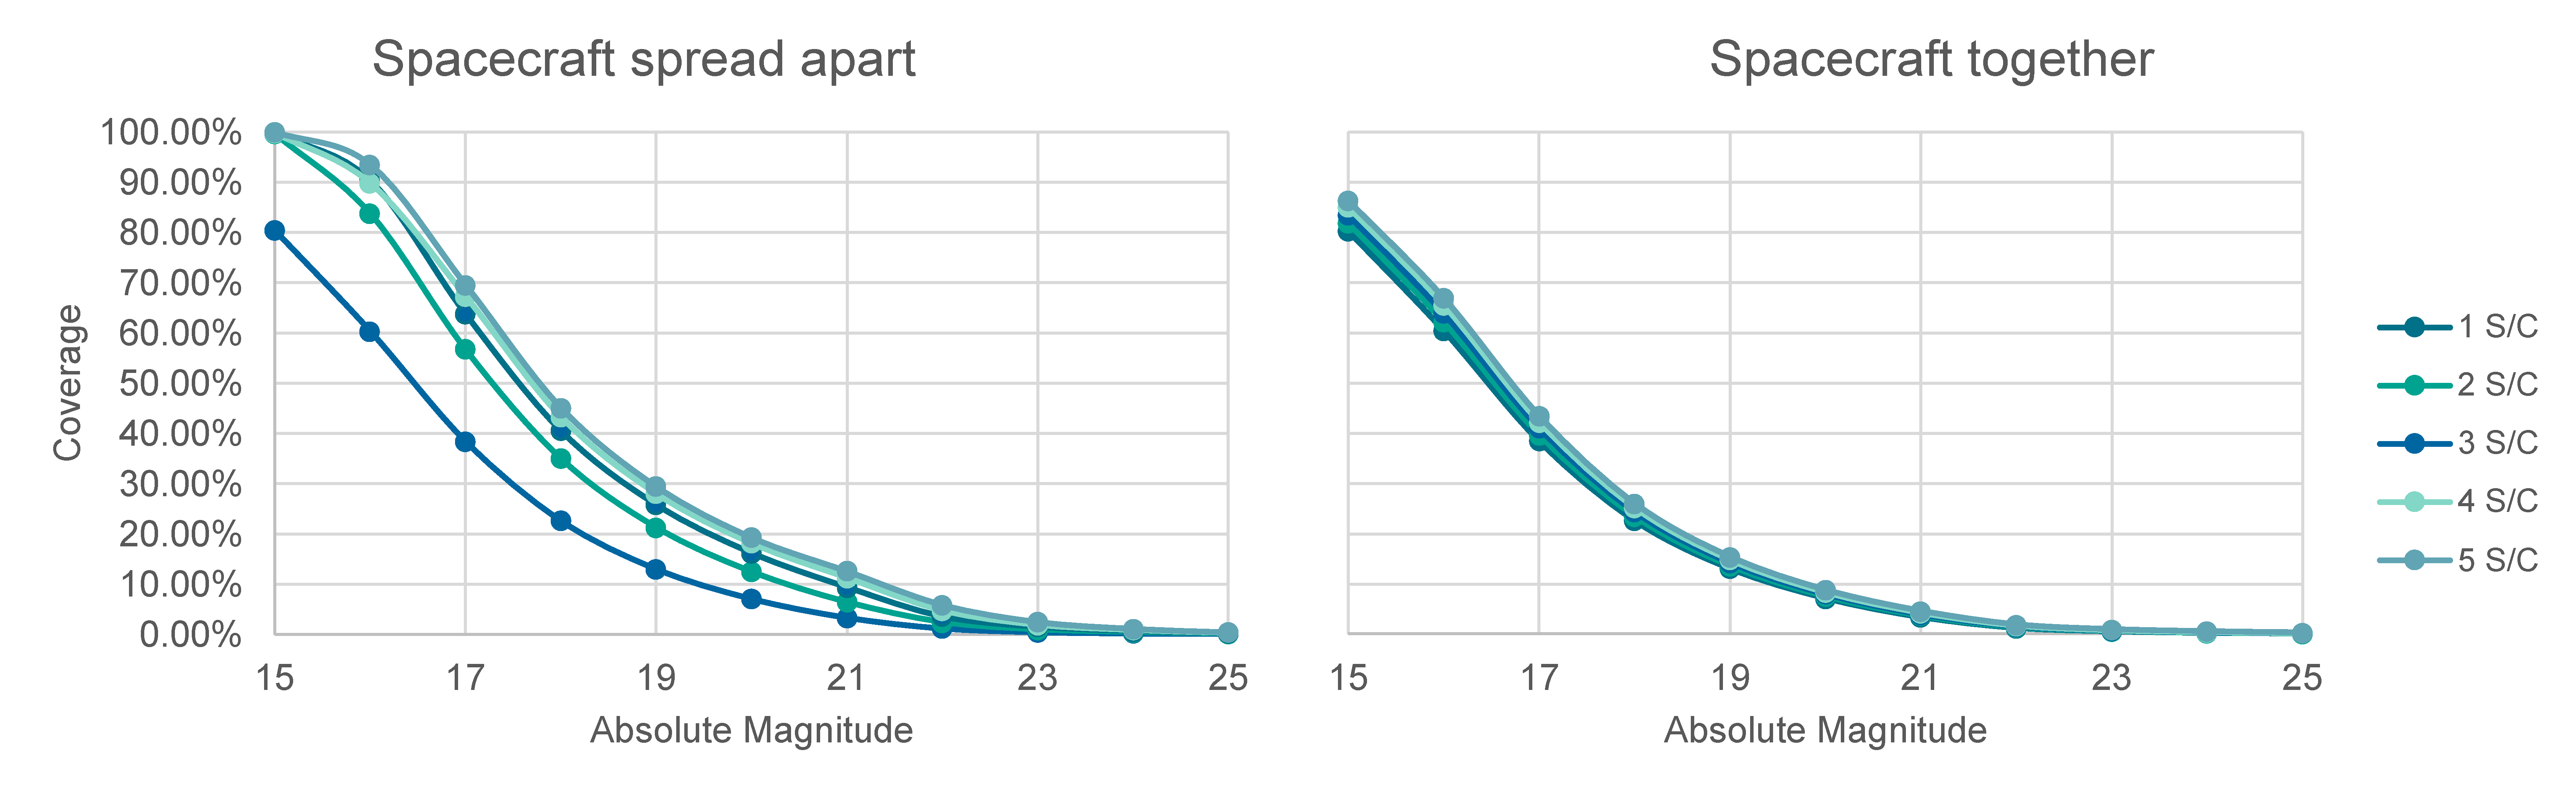
\includegraphics[width=1.0\textwidth]{img/spread_coverage.pdf}
 \caption{Relationship between coverage and asteroid absolute magnitude for spacecraft spread maximally apart, or spread only 0.2 rad}
 \label{fig:spread_coverage}
\end{figure}

The witnessed relationship was investigated numerically, to confirm whether a statistically significant relationship exists, or the effect is merely empirical in nature. For this, a numerical scoring for the coverage was established. This score was set to be the mean of the fraction of the entire area where a certain absolute magnitude can be observed, for absolute magnitude 17-25. That is, with $A_{H}$ the area where an asteroid with absolute magnitude $H$ can be detected at SRN $\geq 5$, and $A_{total}$ the total area, the coverage is defined as:
\begin{equation}
 \mathrm{Coverage} = \frac{1}{25-17}\Sigma_{H=17}^{H=25} \frac{A_{H}}{A_{total}}
\end{equation}
As an example, the coverages at various absolute magnitudes (thus, without the summation) for the above two examples are shown in \autoref{fig:spread_coverage}. It can be seen that indeed, the coverage at all magnitudes is larger for the spread-apart case. And, as established before, the performance is indeed higher for the case with the spacecraft spread apart. To confirm this finding further, a random sampling of a large number of solutions with different semi-major axes, inter-spacecraft spread, and eccentricity, was performed for 2 to 5 spacecraft, and the coverage and completeness was calculated. The results can be seen in \ref{fig:coverage_completeness}. Clearly, a very strong relationship is present between the coverage and the resulting completeness, in addition to a weaker relationship between the number of spacecraft and the completeness (caused by the aforementioned increase in cadence). In other words: the main driver of the survey performance is the volume in space where the system can effectively image asteroids. \\

\begin{figure}[htbp]
 \centering
 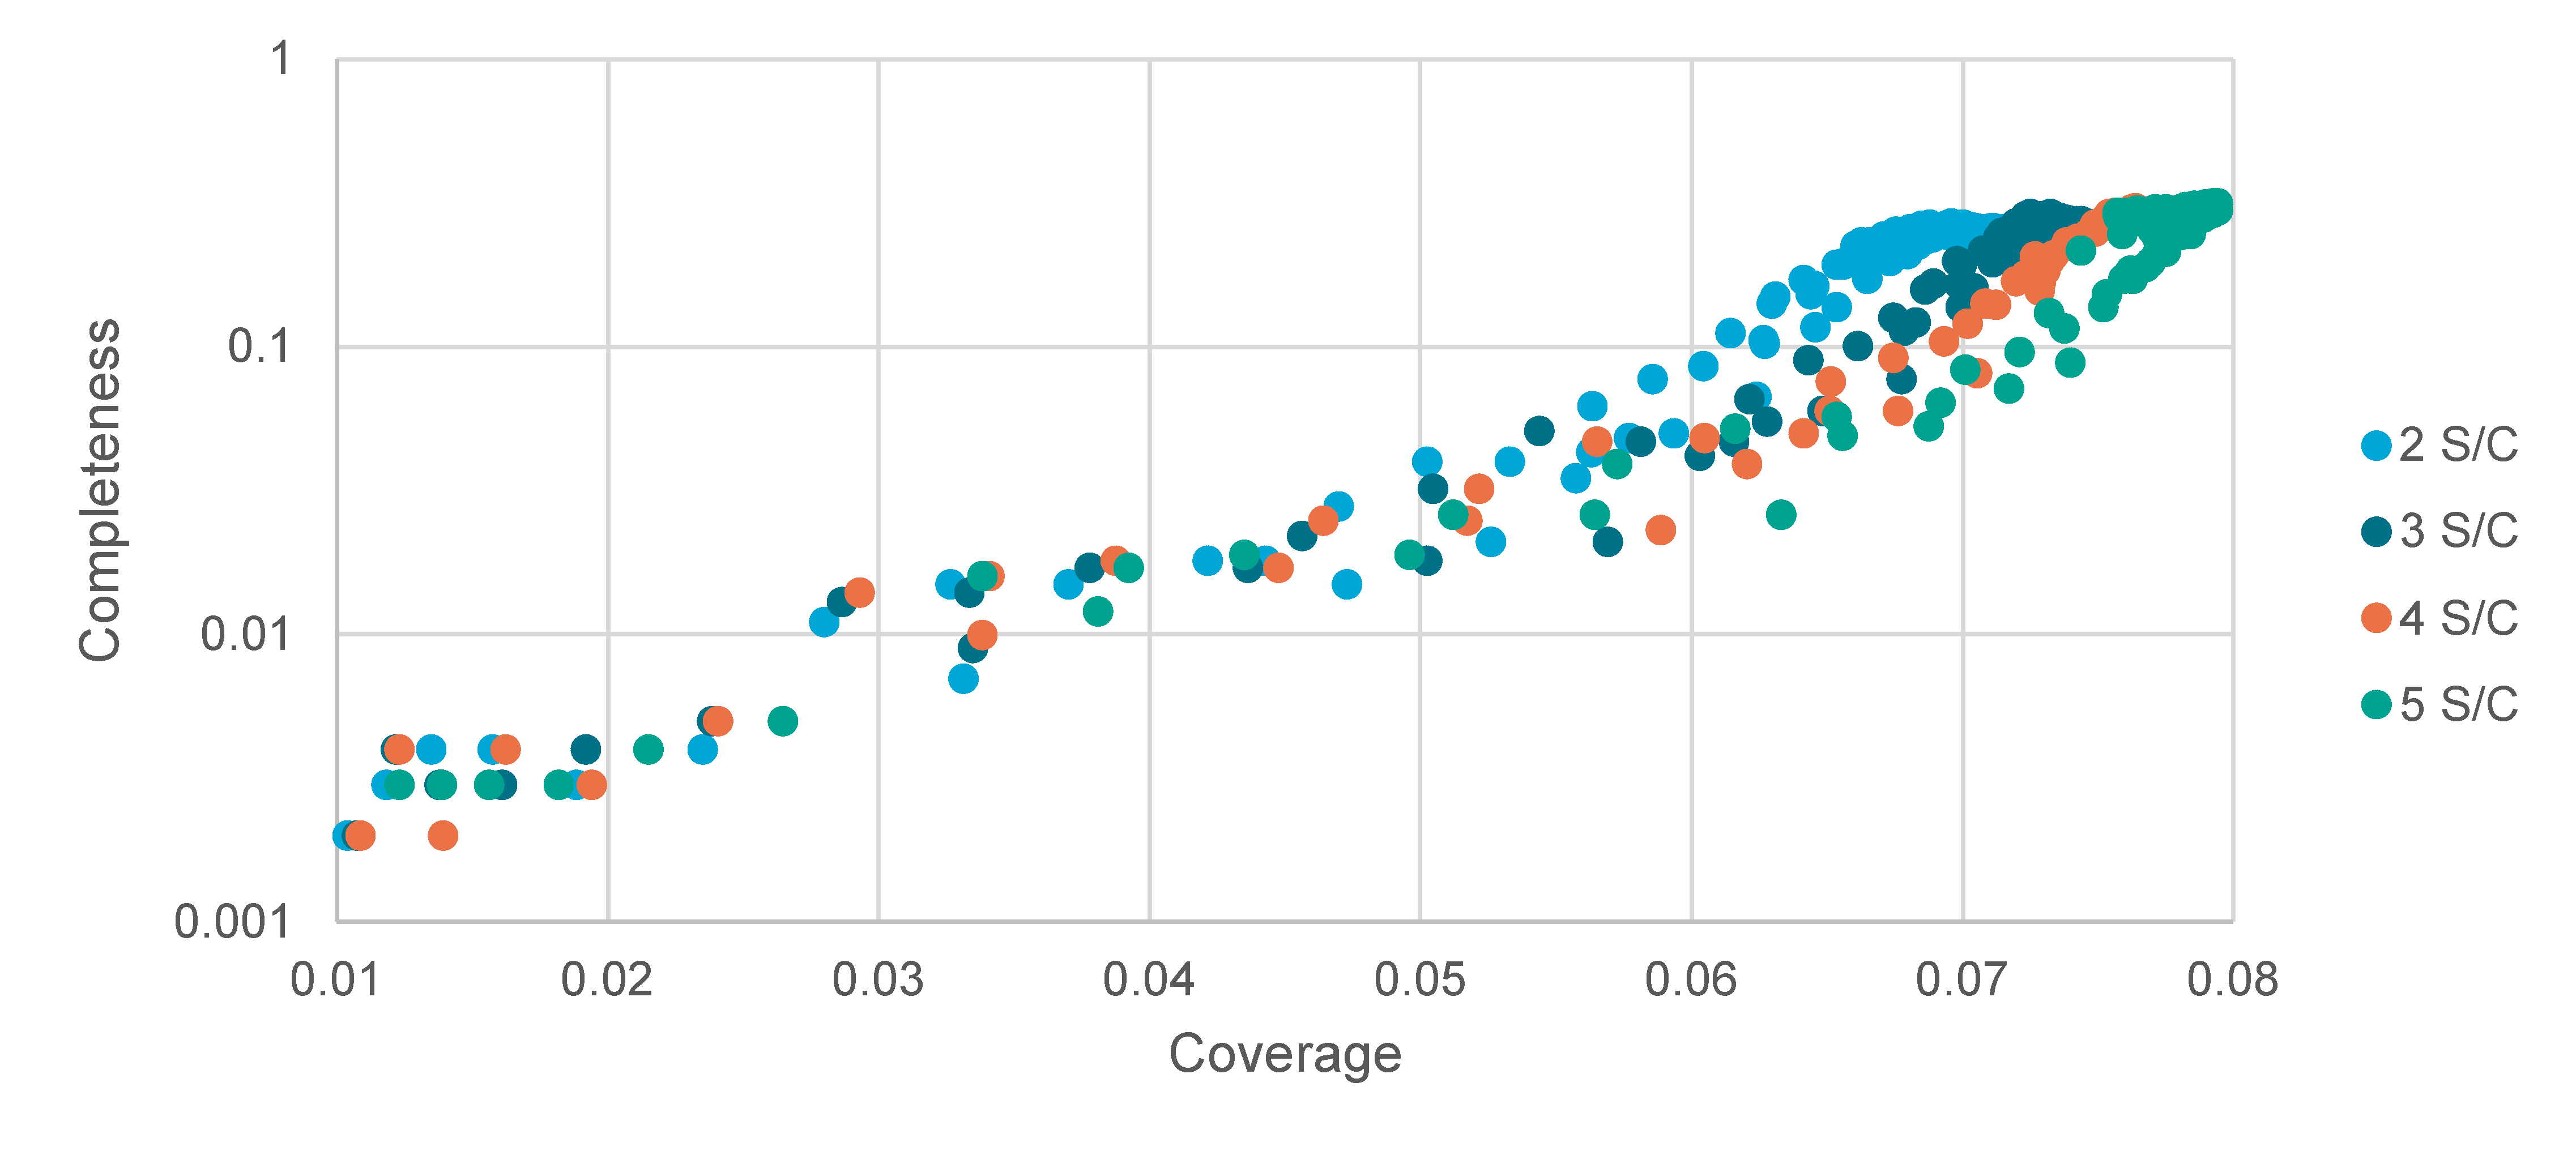
\includegraphics[width=1.0\textwidth]{img/coverage_completeness.pdf}
 \caption{Relationship between coverage and completeness for 2-5 spacecraft. }
 \label{fig:coverage_completeness}
\end{figure}

Working from this relationship, several of the phenomena observed so far can be explained. Firstly indeed the effect of spreading the spacecraft apart as much as possible to minimize the overlap in their search areas. This was already shown previously. Although no statistically significant data is available to confirm this, it is theorized that this is also the reasoning why eccentric orbits do not produce optimal results: As the orbital velocity of the spacecraft is lower near apohelion than near perihelion, the spacecraft in the system will tend to congregate near the apohelion. This then effectively decreases the spread between the spacecraft, increasing the overlap. Secondly, the phenomenon of increasing optimal semi-major axis with larger number of spacecraft can be explained in this way. \autoref{fig:coverage_high_n} shows the resulting coverage for a system of 15 spacecraft, compared to the aforementioned 5 spacecraft, which are shown for reference. It can be seen that as the semi-major axis remains constant, but $n$ increases, a large overlap in the coverage area develops. As the semi-major axis increases, the overlap decreases. Therefore, although individual spacecraft might no longer be in the optimal range, the entire system is capable of detecting asteroids in a larger volume of space, again increasing performance. \\

\begin{figure}[htbp]
 \centering
 \includegraphics[width=1.0\textwidth]{img/coverage_high_n.png}
 \caption{Illustration of the observable area for a system of 15 spacecraft, at a=1.0 AU and a=1.5AU, spread out over the orbit. The 5 spacecraft case is shown for comparison. Coordinates in the $e$ frame, viewing in the negative $Z_e$-direction.}
 \label{fig:coverage_high_n}
\end{figure}

Lastly, this theory can be utilized to provide a prediction about what change in performance is to be expected when optimizing non-co-orbital systems. Such a base prediction is important, as it will help frame the results of the optimizer.  Consider \autoref{fig:coverage_free}: A system is modelled with the semi-major axes of all spacecraft 0.2 AU apart (middle image). Initially, this might seem to cover a larger area than the co-orbital system shown in the left image. Therefore, one would expect it to perform better. However consider the dynamical behavior of the system: As the orbital period of the spacecraft is now different for each spacecraft, they will no longer remain equally spread in space. Over time, spacecraft ``line up'' in a single location, as shown in the right image. It is clear that such a case would be far less preferable than the system in which all spacecraft are situated in the same orbit. Therefore, it is hypothesized that these non-co-orbital solutions will not significantly outperform the co-orbital solutions considered in the previous section.\\

\begin{figure}[htbp]
 \centering
 \includegraphics[width=1.0\textwidth]{img/coverage_free.png}
 \caption{Illustration of the observable area for a system of 5 spacecraft, spread out over the orbit. The left case has the spacecraft co-orbital. In the middle case, the spacecraft are in different orbits, but spread out. On the right, they have lined up in their orbital motion.}
 \label{fig:coverage_free}
\end{figure}

Overall, this theory suggests that the best approach to organizing NEA surveys is to position the spacecraft in such a way as to maximize the volume in which NEAs can be observed. Although this might logically lead to the theory that more complicated orbital arrangements yield better results, this fact is doubtful due to the dynamic behavior of the system reducing the effectiveness over time. One topic here is highlighted which could be investigated for further research: Lagrange points, specifically $L_1$/$L_2$/$L_3$. These points allow the system to utilize slightly different semi-major axes around the Sun, while still maintaining the same orbital periods as other spacecraft in the system, thereby maintaining the distance between the spacecraft. However, due to the additional complication involved in modelling orbits around Lagrange points, modelling of this is left as a recommendation for future research.

\section{Orbital Elements II: Non Co-orbital Spacecraft}
\label{sec:results_orbits_two}

\begin{table}[htbp]
\caption{Overview of optimization parameters for the three investigated optimization cases.}
\label{tab:optimizationcases}
\begin{tabulary}{1.0\textwidth}{L|L|L|L|L}
\textbf{Case}                & \textbf{Semi-major axis}             & \textbf{Eccentricity}            & \textbf{Anomaly at epoch}        & \textbf{Number of parameters} \\ \hline
Circular, co-orbital         & 1 optimization parameter for all S/C & 0                                & Spread evenly over the orbit     & 1                             \\
Circular, non-co-orbital     & 1 optimization parameter per S/C     & 0                                & 1 optimization parameter per S/C & 2n                            \\
Non-circular, non-co-orbital & 1 optimization parameter per S/C     & 1 optimization parameter per S/C & 1 optimization parameter per S/C & 3n
\end{tabulary}
\end{table}

Although the aforementioned analysis predicts a detrimental effect on performance, it is nevertheless logical to extend the analysis presented in \autoref{sec:results_orbits_one} to non-co-orbital configurations. This complicates the analysis significantly, as the dimensionality of the problem rapidly increases. Therefore, special attention has to be paid to the performance of the optimizer, and validation tests should be run on its results. In addition, to aid in comparison, three sets of optimization parameters were analysed. Firstly, a circular, co-orbital case: a system which has all spacecraft spread out as much as possible, in a single circular orbit. From the results in the previous section, it follows that this is the optimal co-orbital solution. Secondly, a circular, non-co-orbital case: a system in which each spacecraft can have a distinct semi-major axis and anomaly at epoch. Because spacecraft with different semi-major axes have different orbital periods, the spacecraft can not be spread out equally a priori. Therefore, the optimizer has to take care of this task as well, and not just the semi-major axes. Lastly, a non-circular, non-co-orbital case: a similar set of parameters is analysed, but with orbits that are allowed to be non-circular. In that case, the parameter space comprises a semi-major axis, true anomaly at epoch, and eccentricity for each spacecraft. An overview of the different optimization cases is given in \autoref{tab:optimizationcases}.\\

\begin{figure}[htbp]
 \centering
 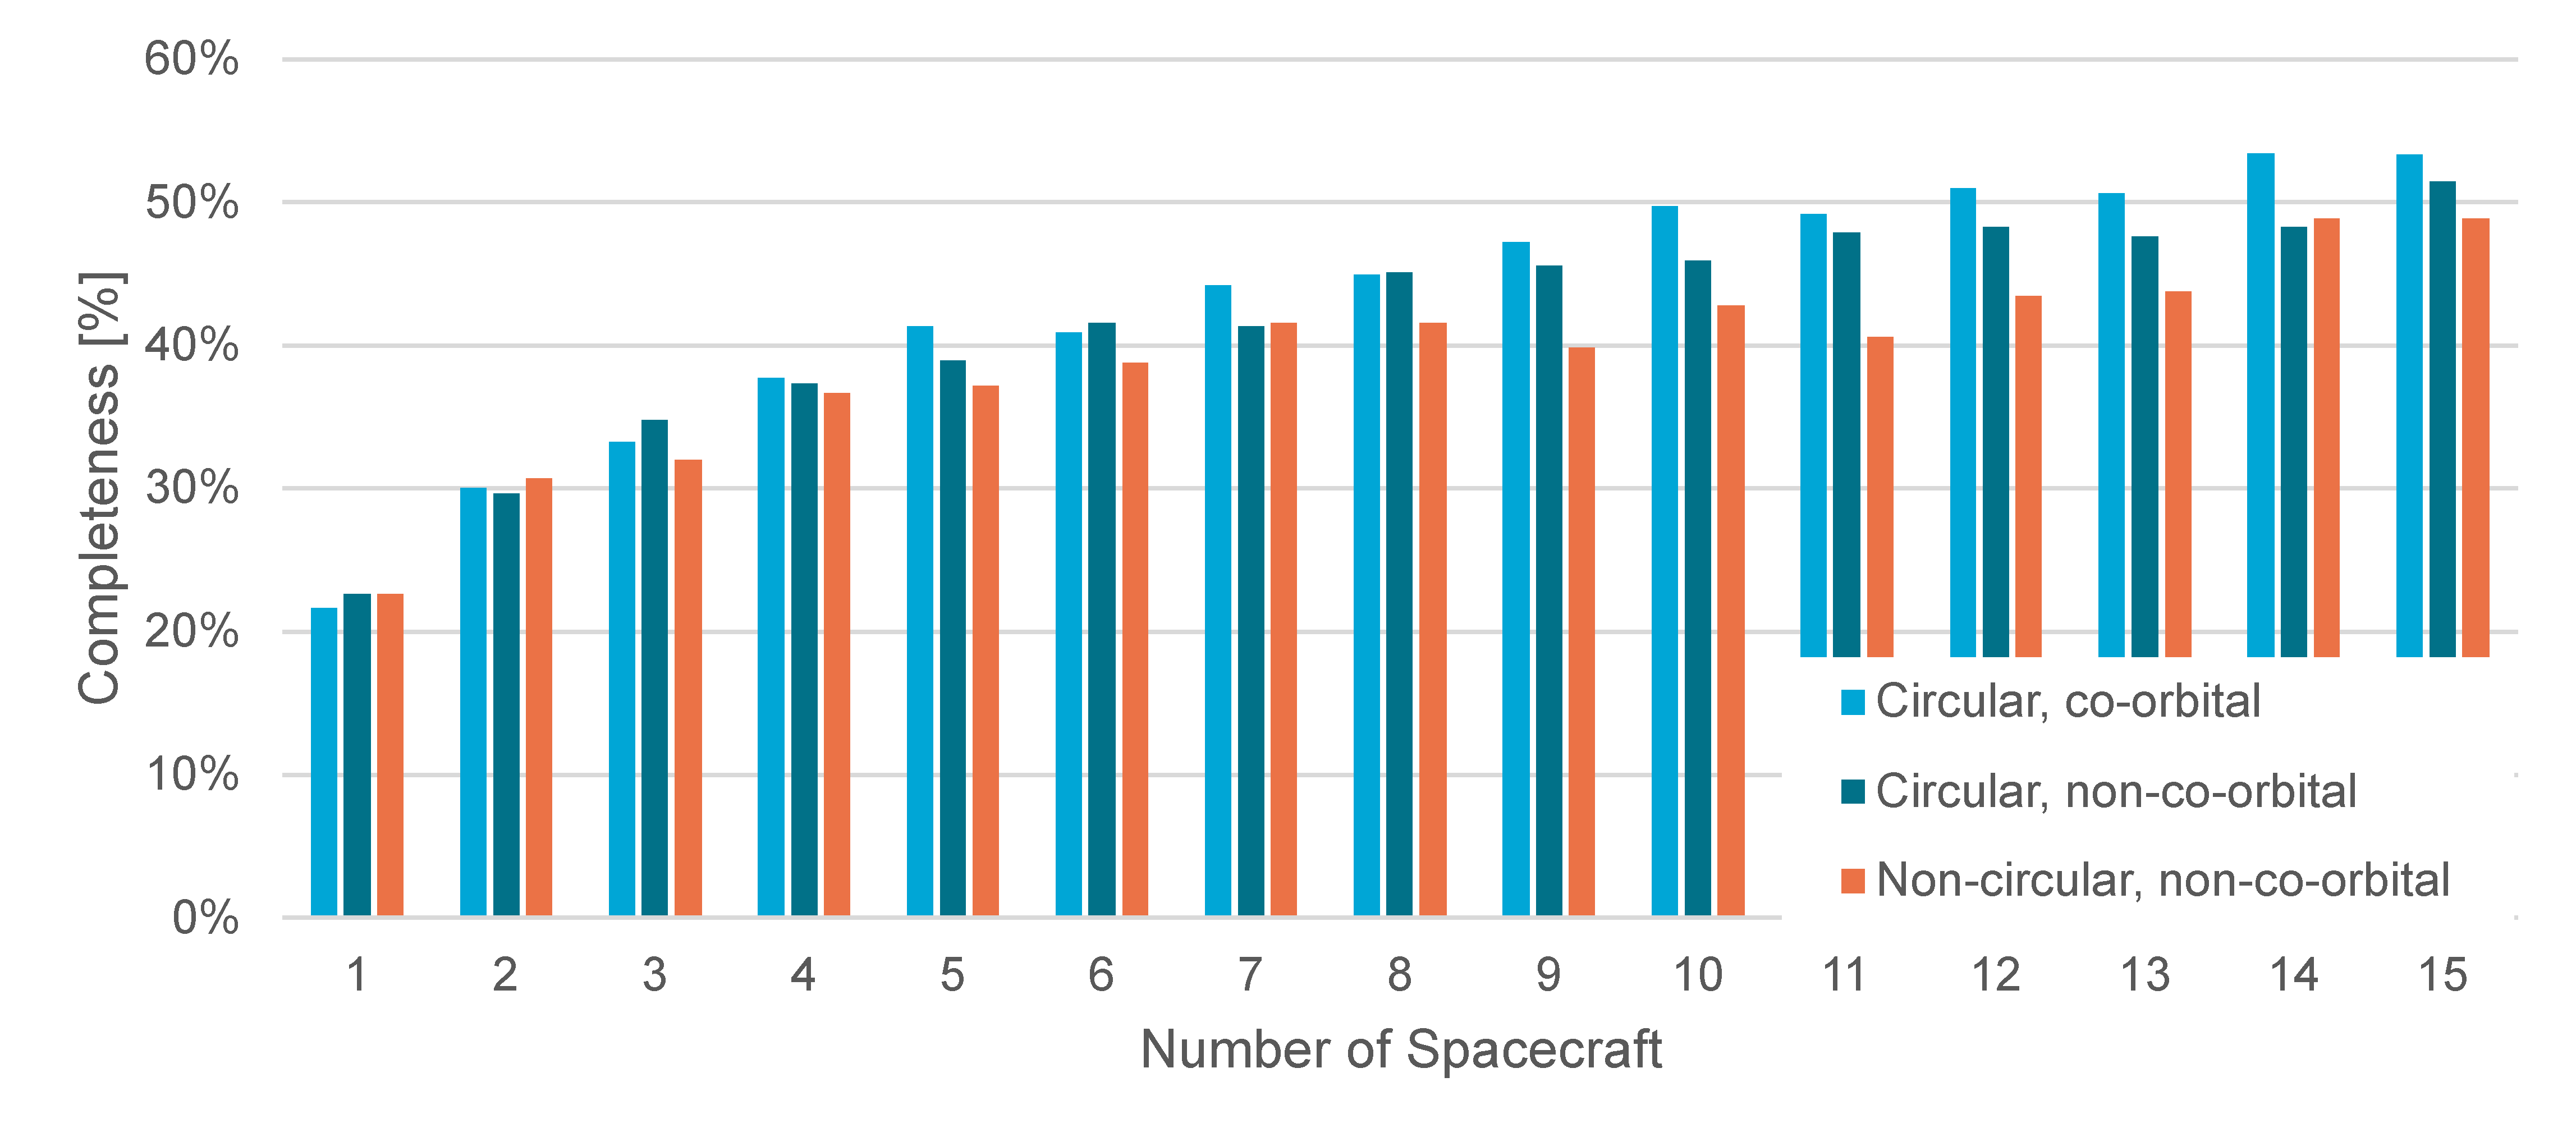
\includegraphics[width=1.0\textwidth]{img/performance_free.pdf}
 \caption{Performances for systems optimized for either a single semi-major axis, distinct semi-major axes and anomalies per spacecraft, or distinct semi-major axes, anomalies and eccentricities per spacecraft.}
 \label{fig:performance_free}
\end{figure}

The results of the optimization processes can be seen in \autoref{fig:performance_free}. It can be seen that several performance breakpoints are present: for low numbers of spacecraft, approximately $1 \leq n \leq 5$, all three methods result in similar performances. Then, for approximately $6 \leq n \leq 10$, the performance of the optimization for the non-circular, non-co-orbital case starts degrading relative to the other two. Lastly, for $n > 10$, the circular, co-orbital solution is superior to the other two methods. These results might be surprising to some readers: one would expect the performance to either increase, or stay equal, as more parameters become available to the optimizer. After all, all solutions found for a circular, co-orbital system of spacecraft (i.e. only a single semi-major axis gets determined by the optimizer), can be recreated by the other two optimizers, and therefore they can reach the same performance. The source of this discrepancy is twofold. The first aspect is the problem of the optimizer overfitting to the noise in the system. The second aspect is related to the actual performance benefits obtainable through these more complex solutions. Although the results here might seem inconclusive, the combination of both aspects will allow supporting the hypothesis presented in the previous section.\\

\begin{figure}[htbp]
 \centering
 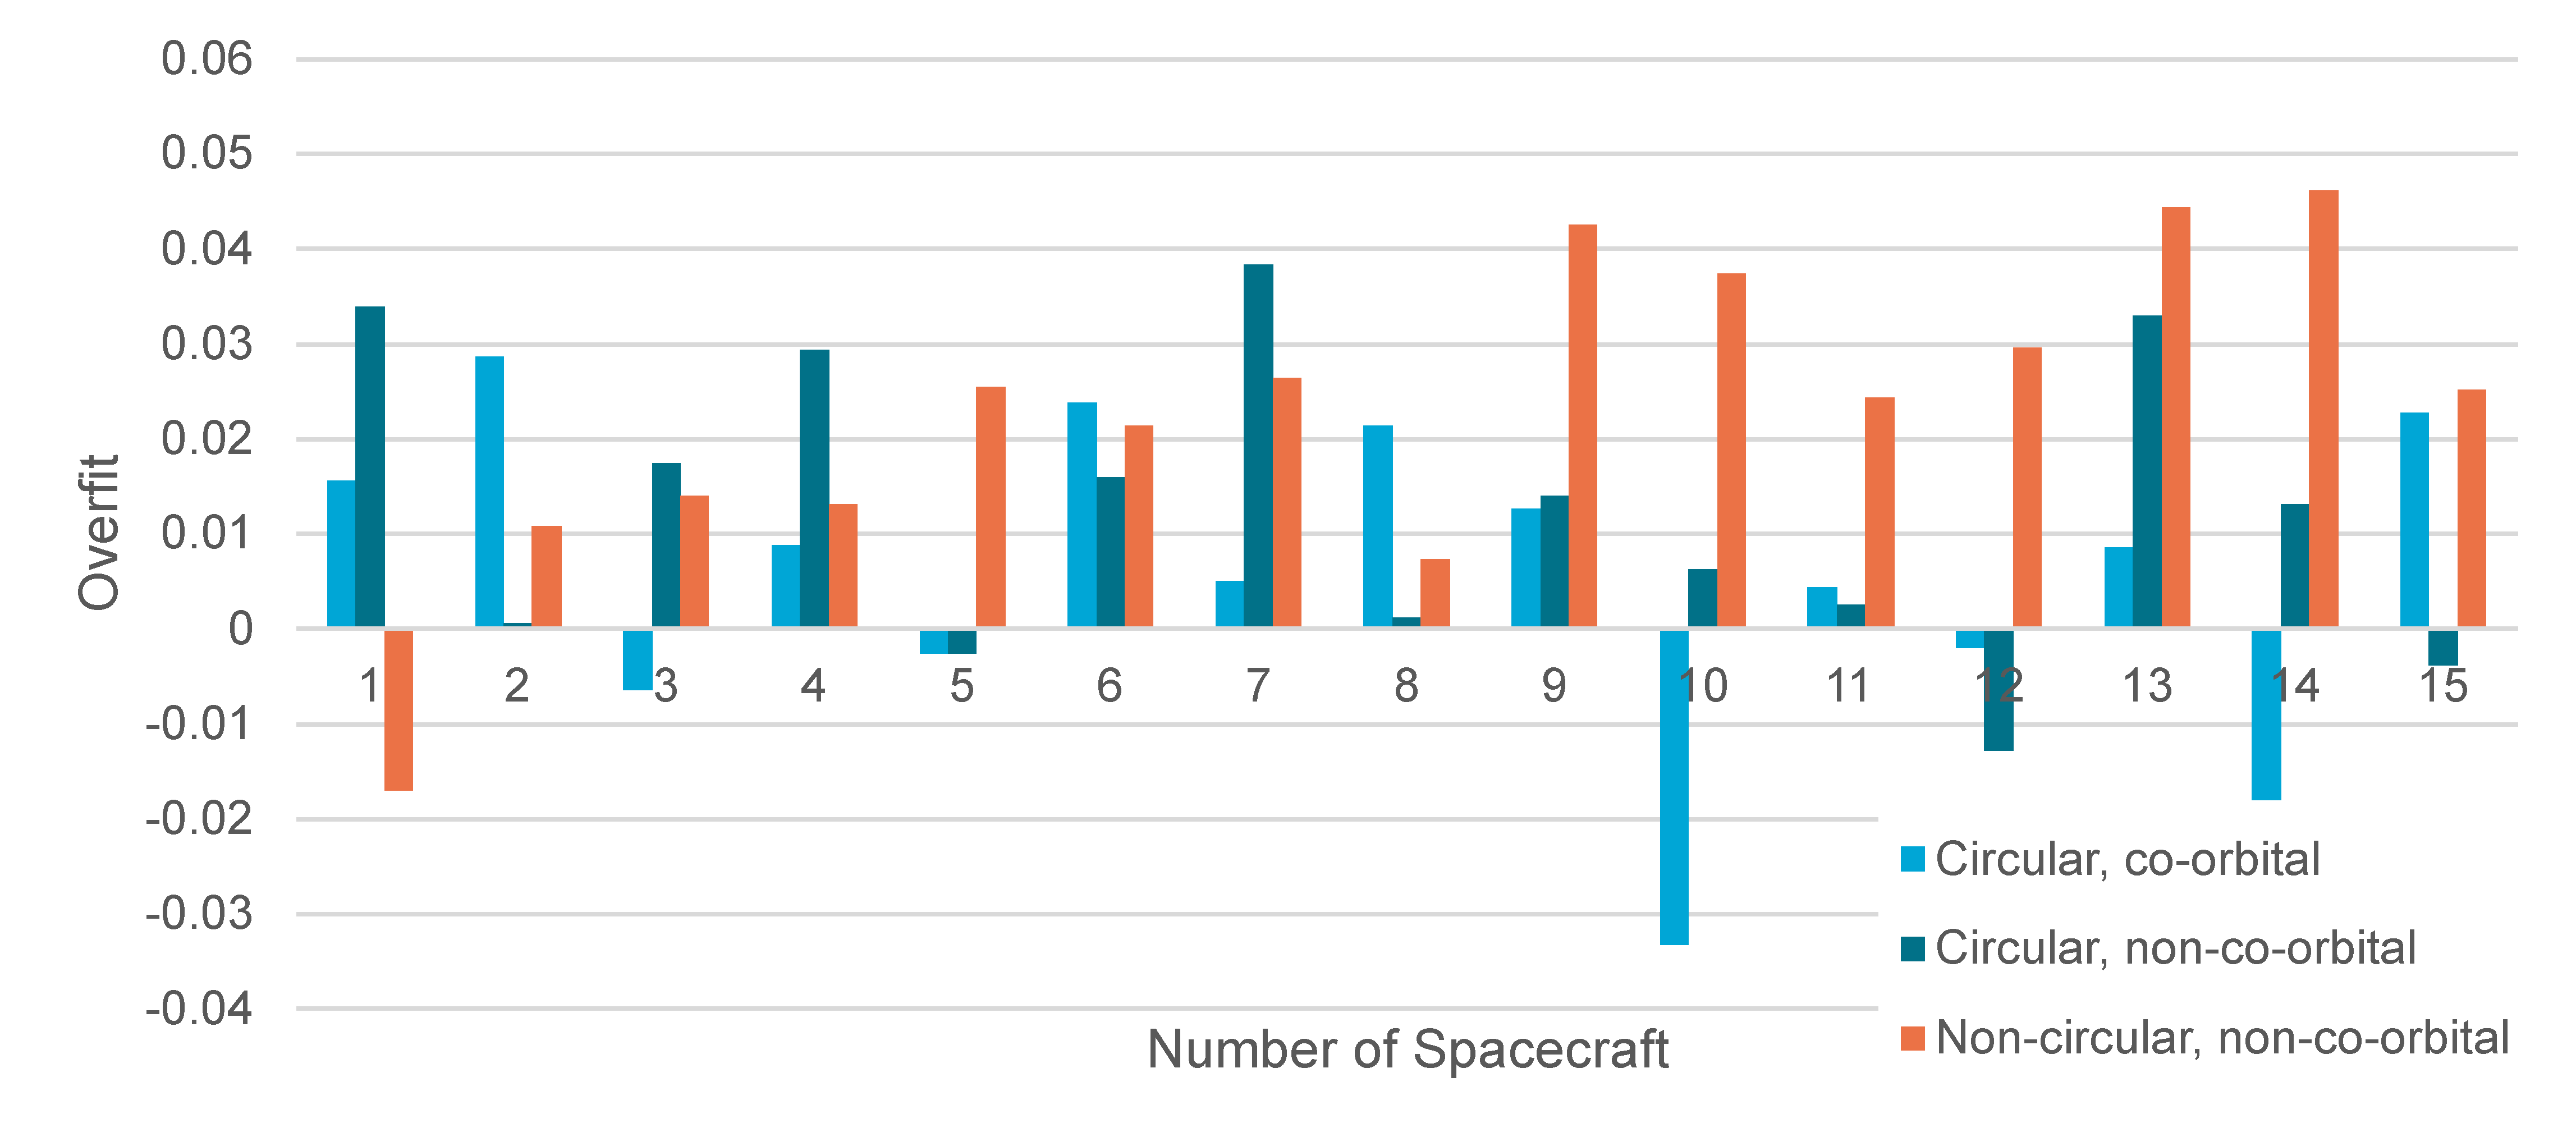
\includegraphics[width=1.0\textwidth]{img/overfit_free.pdf}
 \caption{Overfit of the optimizer per number of spacecraft.}
 \label{fig:overfit_free}
\end{figure}
\begin{figure}[htbp]
 \centering
 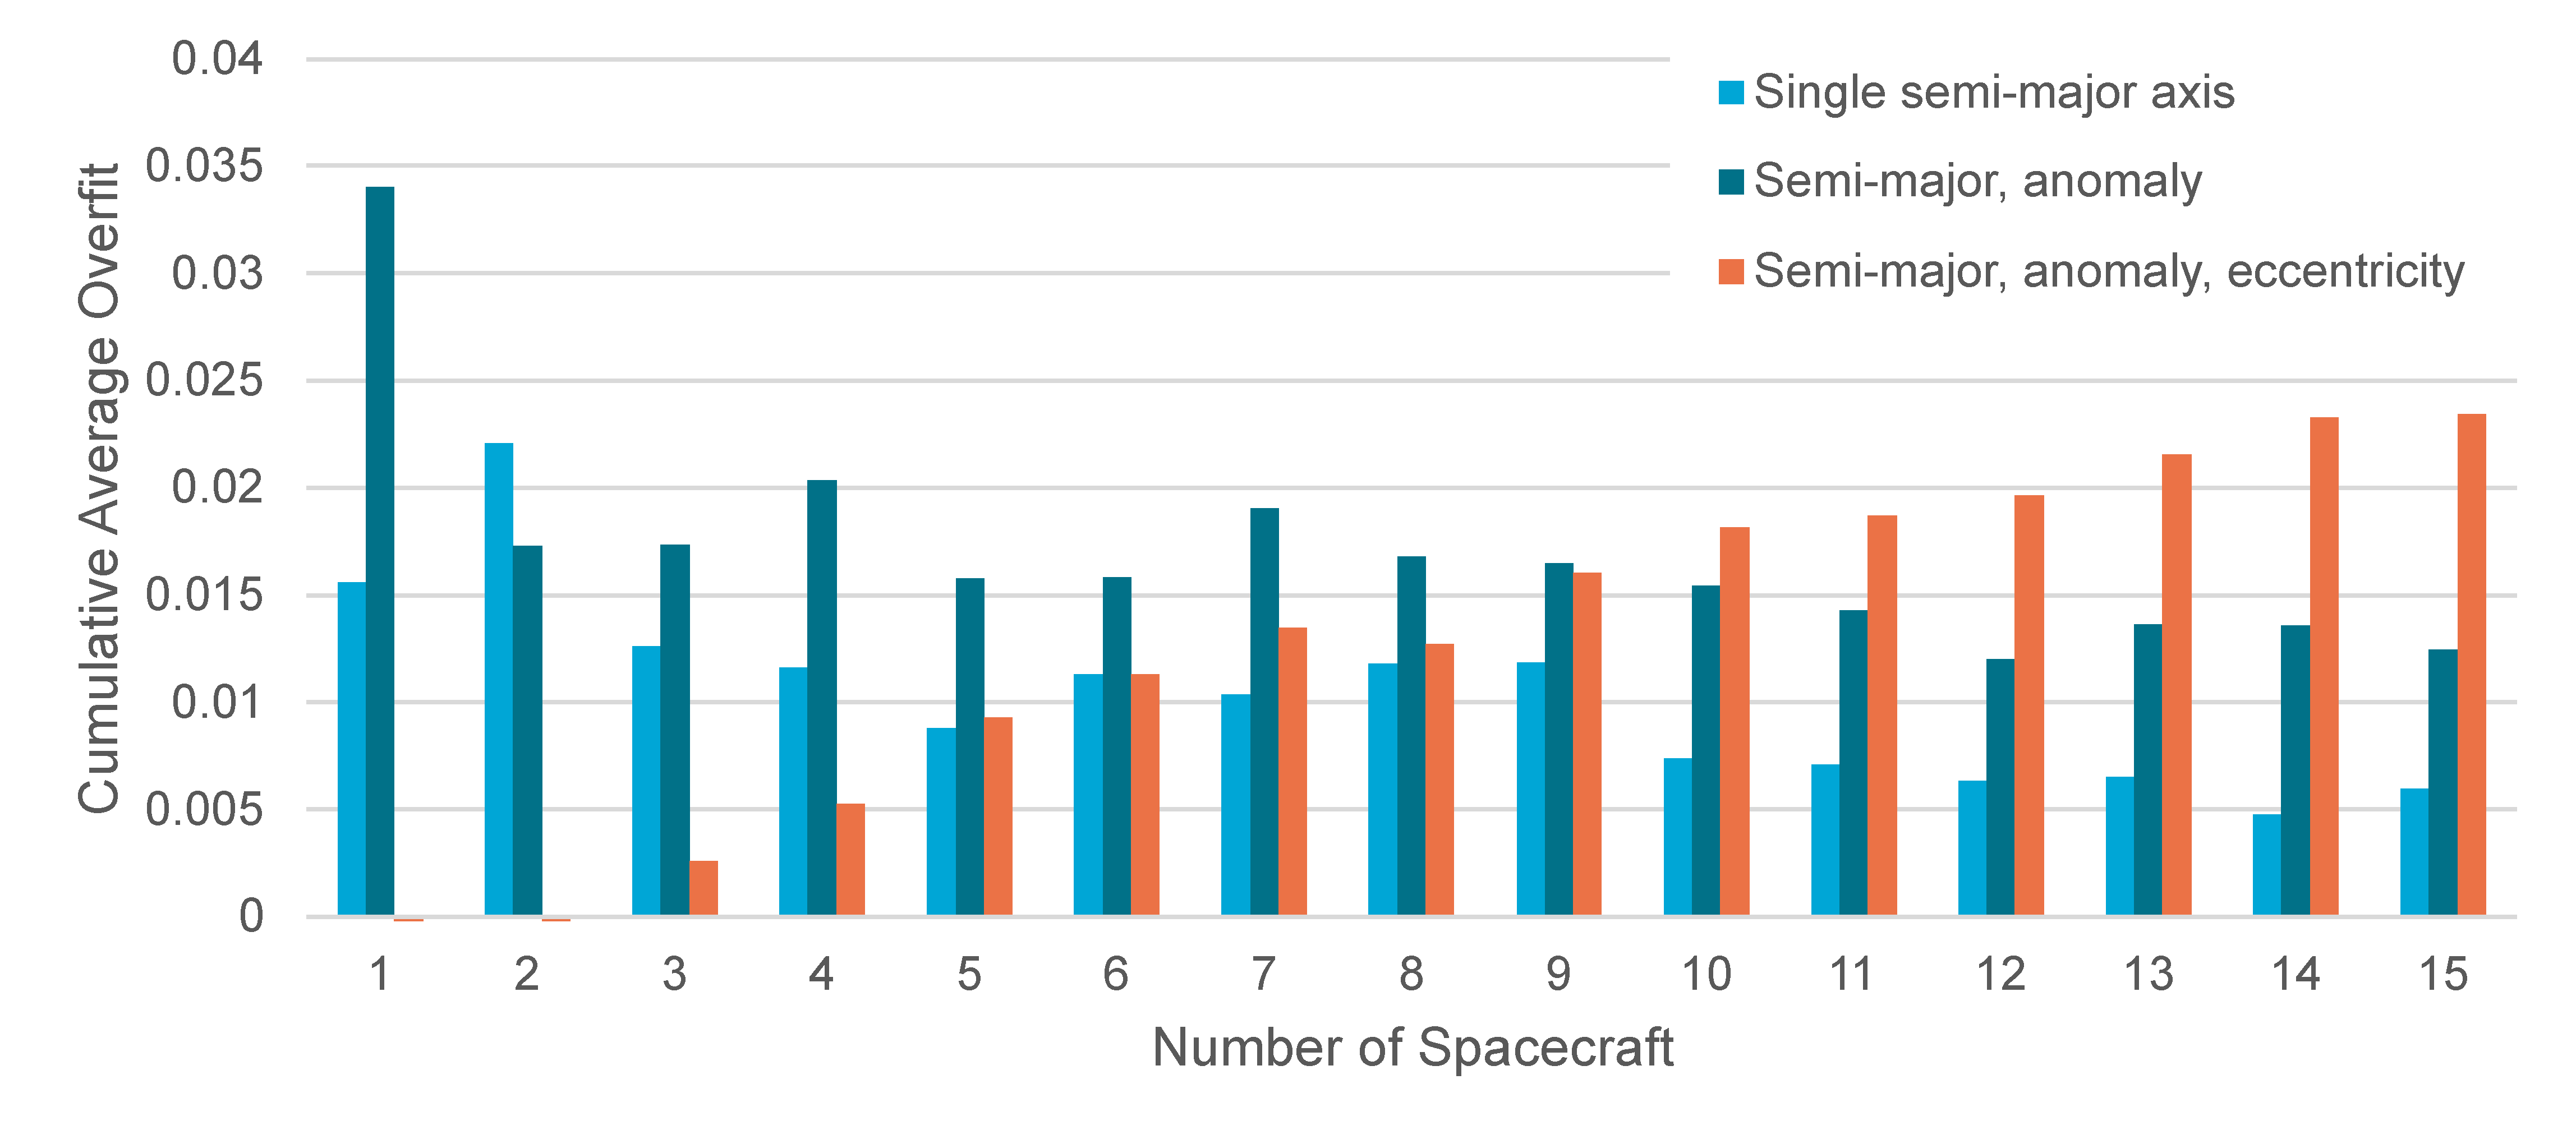
\includegraphics[width=1.0\textwidth]{img/overfit_free_cumulative_average.pdf}
 \caption{Cumulative average of the overfit of the optimizer per number of spacecraft.}
 \label{fig:overfit_free_cumulative_average}
\end{figure}

First, the problem of overfit will be adressed. To illustrate the occurence of overfit at higher dimensionalities, \autoref{fig:overfit_free} gives the overfit for each optimization problem, per spacecraft. Overfit is defined simply as the difference between the learning performance (i.e. the performance predicted by the optimizer for its solution) and the validation performance (the actual performance which can be expected at the solution). As \autoref{fig:overfit_free} is hard to interpret directly, \autoref{fig:overfit_free_cumulative_average} provides the cumulative average up to and including a certain number of spacecraft. Several observations are made here:
\begin{itemize}
 \item As the number of spacecraft increases, the average overfit of the circular, co-orbital system decreases. In other words, for a higher number of spacecraft, the optimizer performs better. This occurs because, in this system, the dimensionality does not increase (as can be seen in \autoref{tab:optimizationcases}, the total number of optimization parameters in this case is always 1), and therefore the task of the optimizer is equally hard. However, as the distribution of spacecraft becomes more uniform, the system will overfit less to the population as the importance of the starting position of each spacecraft becomes smaller: As the population is not exactly radially symmetric, a difference in performance can be expected based on the start position. However, for higher numbers of spacecraft, the variation which is possible with regards to the system becomes smaller, as the angular distance between the spacecraft (and therefore the possible radial asymmetry) is smaller. Therefore, a higher number of spacecraft incurs a regularizing effect on the optimizer.
 \item Secondly, the average overfit of the circular, non-co-orbital system, exhibits no statistically significant slope. The degree of overfit levels out around 1-1.5\%. At this degree of overfitting, the optimizer is capable of finding a solution to the problem.
 \item Lastly, the non-circular, non-co-orbital system shows an \textit{increase} in overfitting. I.e., the optimizer is not capable of keeping up with the increasing dimensionality of the problem, and the quality of the result continually decreases.
\end{itemize}
Before investigating the second point, first some of the solutions of the optimizer will be examined, along with their training progress. Note that in the learning/validation graphs, ``epoch'' refers to the step in the learning process, not the datum of the astronomical coordinate system. The solutions to be investigated are two, six and eleven spacecraft. The one spacecraft case is omitted as the optimal solution is already known from previous analysis to be the optimal solution to the single semi-major axis system. The six and eleven spacecraft cases were chosen as they represent the first solution after the performance breakpoints discussed earlier. Optimization solutions for all numbers of spacecraft investigated, along with the learning/validation curves, can be found in \autoref{ch:appendix}.
\begin{figure}[htbp]
 \centering
 \includegraphics[width=1.0\textwidth]{img/orbits_2.png}
 \caption{Optimization results for systems with two spacecraft.}
 \label{fig:orbits_2}
\end{figure}
\begin{figure}[htbp]
 \centering
 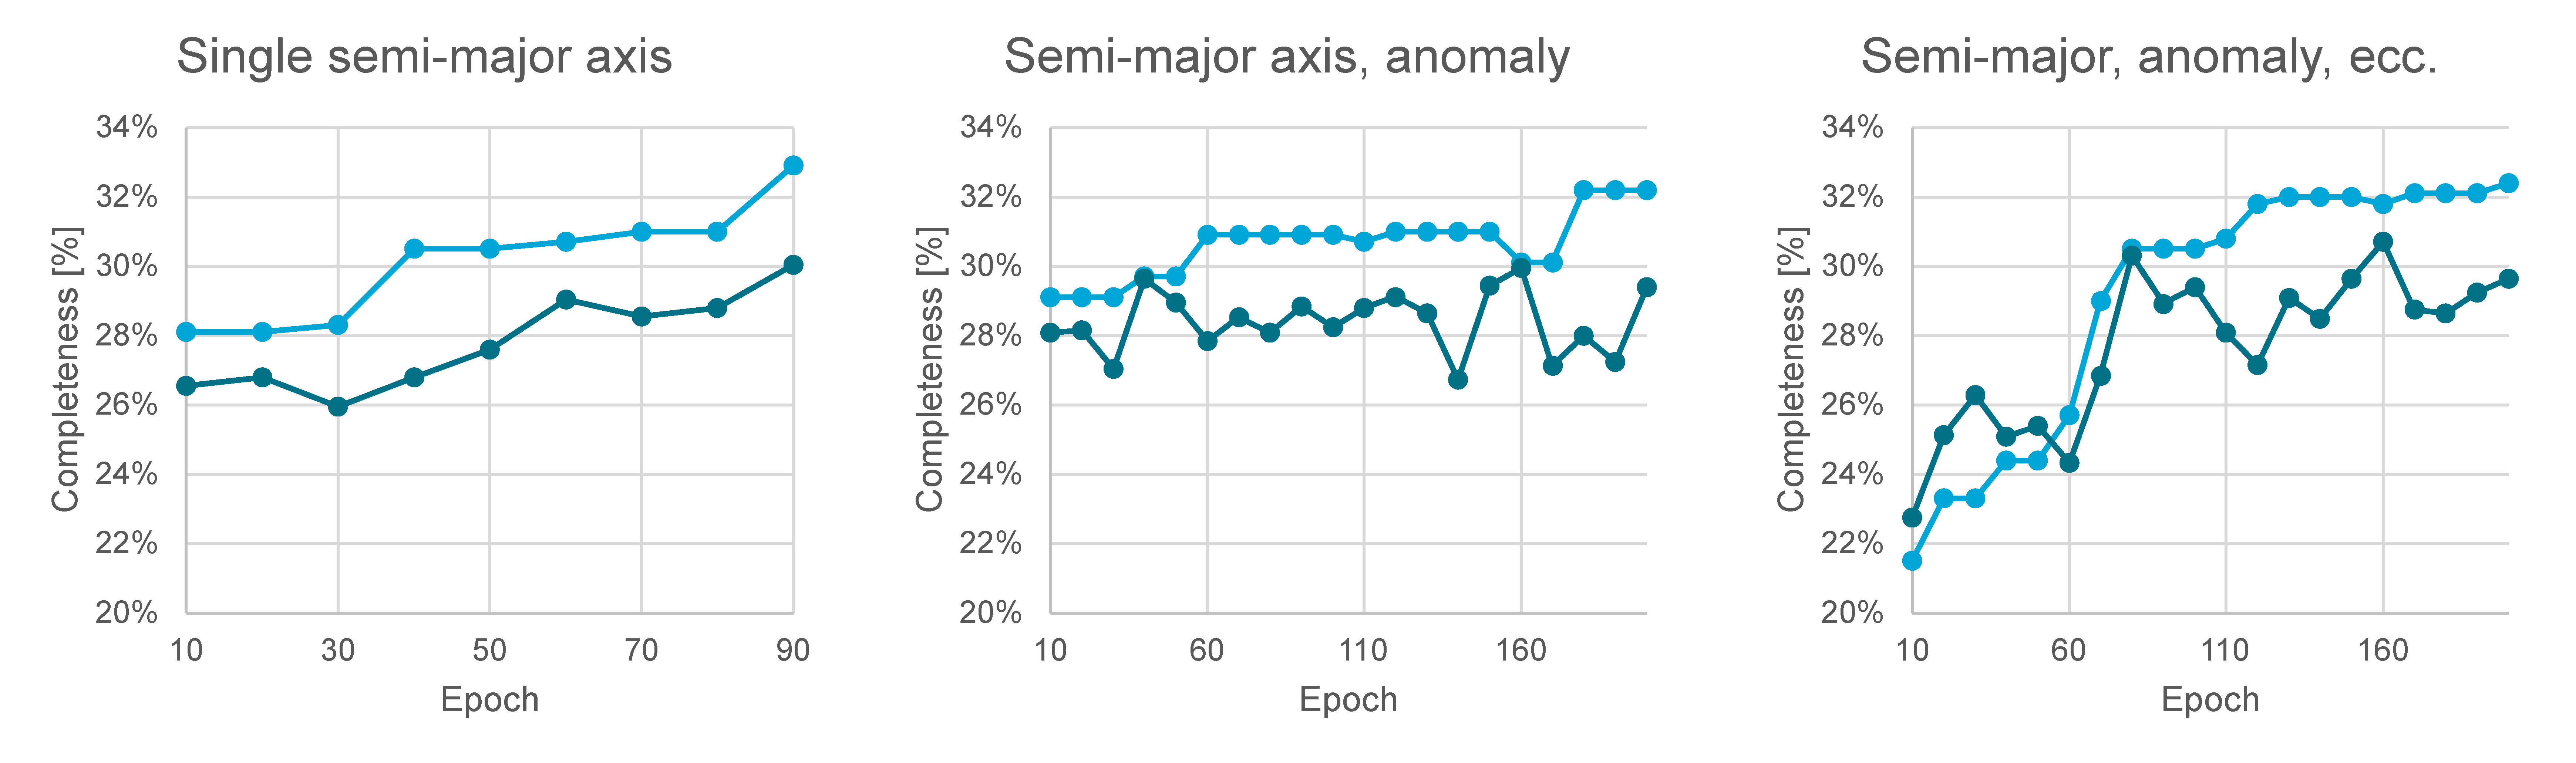
\includegraphics[width=1.0\textwidth]{img/val_orbits_2.pdf}
 \caption{Learning/validation results for systems with two spacecraft.}
 \label{fig:val_orbits_2}
\end{figure}

\begin{table}[htbp]
\centering
\caption{Optimization results for 2 spacecraft.}
\label{tab:opt_2}
\begin{tabulary}{1.0\textwidth}{L|LLL}
                             & $a$   & $e$   & $\theta$ \\ \hline
circular, co-orbital         & 0.922, 0.922 & 0.000, 0.000 & 0.000, 3.142   \\
circular, non-co-orbital     & 0.941, 0.941 & 0.000, 0.000 & 2.486, 2.891   \\
non-circular, non-co-orbital & 1.029, 0.964 & 0.012, 0.100 & 3.609, 3.488  
\end{tabulary}
\end{table}

Firstly, the case for two spacecraft. The solutions and associated learning and validation curves are shown in \autoref{fig:orbits_2} and \autoref{fig:val_orbits_2}. The orbital parameters can be found in \autoref{tab:opt_2}. The circular, co-orbital case can be seen to be optimizing well. The circular, non-co-orbital does place the spacecraft in the same orbit, but closer together. When examining the validation curve, it can be seen that later learning steps do not result in a better validation score, indicating overfitting. This is most likely because the increase in performance from spreading the spacecraft further apart is smaller than the variance in the results. Lastly, the non-circular, non-co-orbital case, which also has access to eccentricity, still behaves well. Instead of a circular solution, one of the spacecraft is placed on a slightly eccentric orbit. This yields a similar performance. In addition, although the optimizer is still well behaved, it takes a large number of steps to reach its eventual solution. \\

\begin{figure}[htbp]
 \centering
 \includegraphics[width=1.0\textwidth]{img/orbits_6.png}
 \caption{Optimization results for systems with six spacecraft.}
 \label{fig:orbits_6}
\end{figure}
\begin{figure}[htbp]
 \centering
 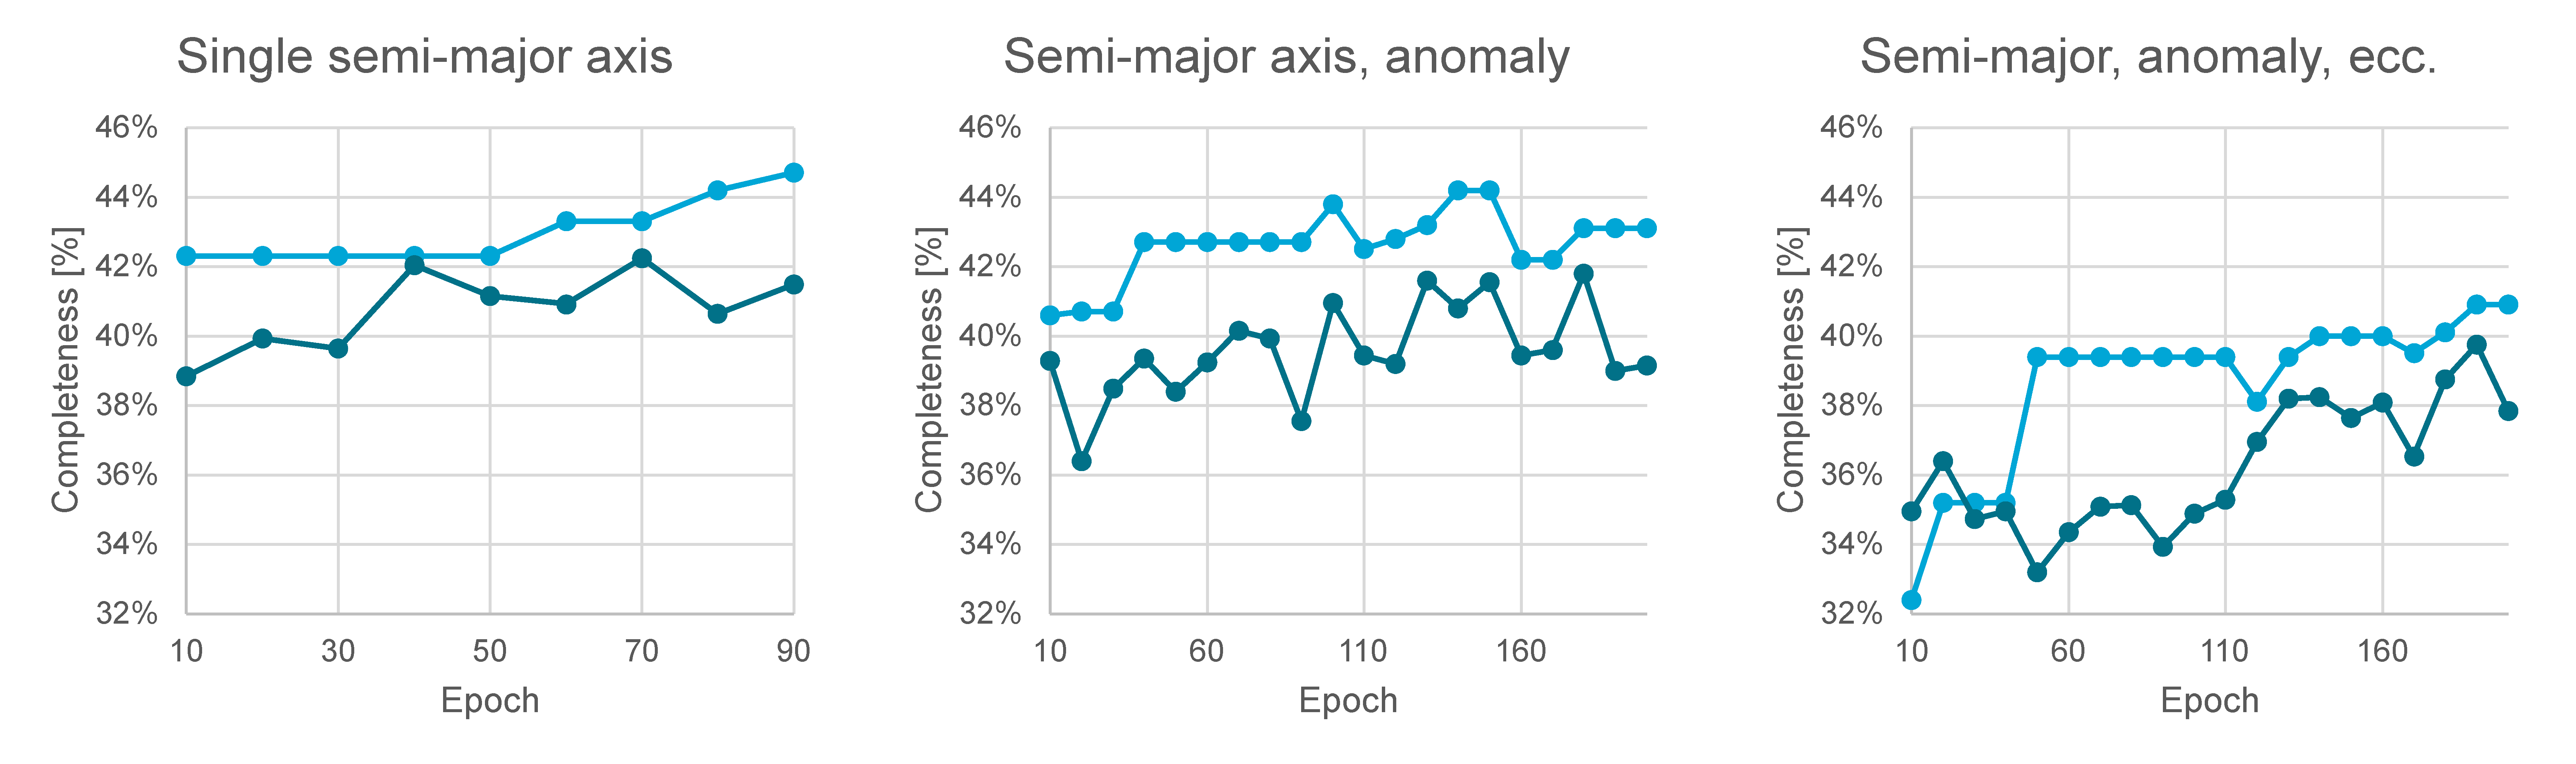
\includegraphics[width=1.0\textwidth]{img/val_orbits_6.pdf}
 \caption{Learning/validation results for systems with six spacecraft.}
 \label{fig:val_orbits_6}
\end{figure}

\begin{table}[htbp]
\centering
\caption{Optimization results for 6 spacecraft.}
\label{tab:opt_6}
\begin{tabulary}{1.0\textwidth}{L|LLL}
                             & $a$                                          & $e$                                          & $\theta$                                      \\ \hline
circular, co-orbital         & 1.170,   1.170, 1.170, 1.170, 1.170, 1.170 & 0.000, 0.000, 0.000, 0.000,   0.000, 0.000 & 0.000, 1.047, 2.094, 3.142,   4.189, 5.236 \\
circular, non-co-orbital     & 1.066,   1.154, 1.104, 1.444, 0.657, 1.510 & 0.000, 0.000, 0.000, 0.000,   0.000, 0.000 & 5.254, 2.511, 1.162, 2.496,   6.469, 2.533 \\
non-circular, non-co-orbital & 0.947,   1.117, 1.156, 0.558, 0.767, 1.194 & 0.051, 0.629, 0.119, 0.562,   0.533, 0.155 & 4.108, 1.860, 0.073, 2.158,   0.811, 5.757
\end{tabulary}
\end{table}

The second case to be examined is the case of six spacecraft. \autoref{fig:orbits_6} and \autoref{fig:val_orbits_6} show the orbits and learning curves, respectively, and \autoref{tab:opt_6} lists the found orbital parameters. As seen in the performance predictions earlier, both circular cases still yield good results for this number of spacecraft, although the non-circular case is starting to underperform. This can be seen in the learning curves. Not only does the non-circular, non-co-orbital system fail to obtain a good solution from the beginning - it's learning performance is also lower than the other two systems - the optimizer struggles to improve the solution through iteration. The resulting orbits provide some insight into what is happening: some of the spacecraft are still in useful positions, however a part is placed on highly eccentric orbits. It has been shown already that these orbits are not a positive addition to the system, and they are most likely the result of overfitting. When considering the circular, non-co-orbital system, interestingly it can be seen that the system still chooses to place some of the spacecraft in the same orbit. However, it also fails to find a solution which outperforms the co-orbital case. \\

\begin{figure}[htbp]
 \centering
 \includegraphics[width=1.0\textwidth]{img/orbits_11.png}
 \caption{Optimization results for systems with eleven spacecraft.}
 \label{fig:orbits_11}
\end{figure}
\begin{figure}[htbp]
 \centering
 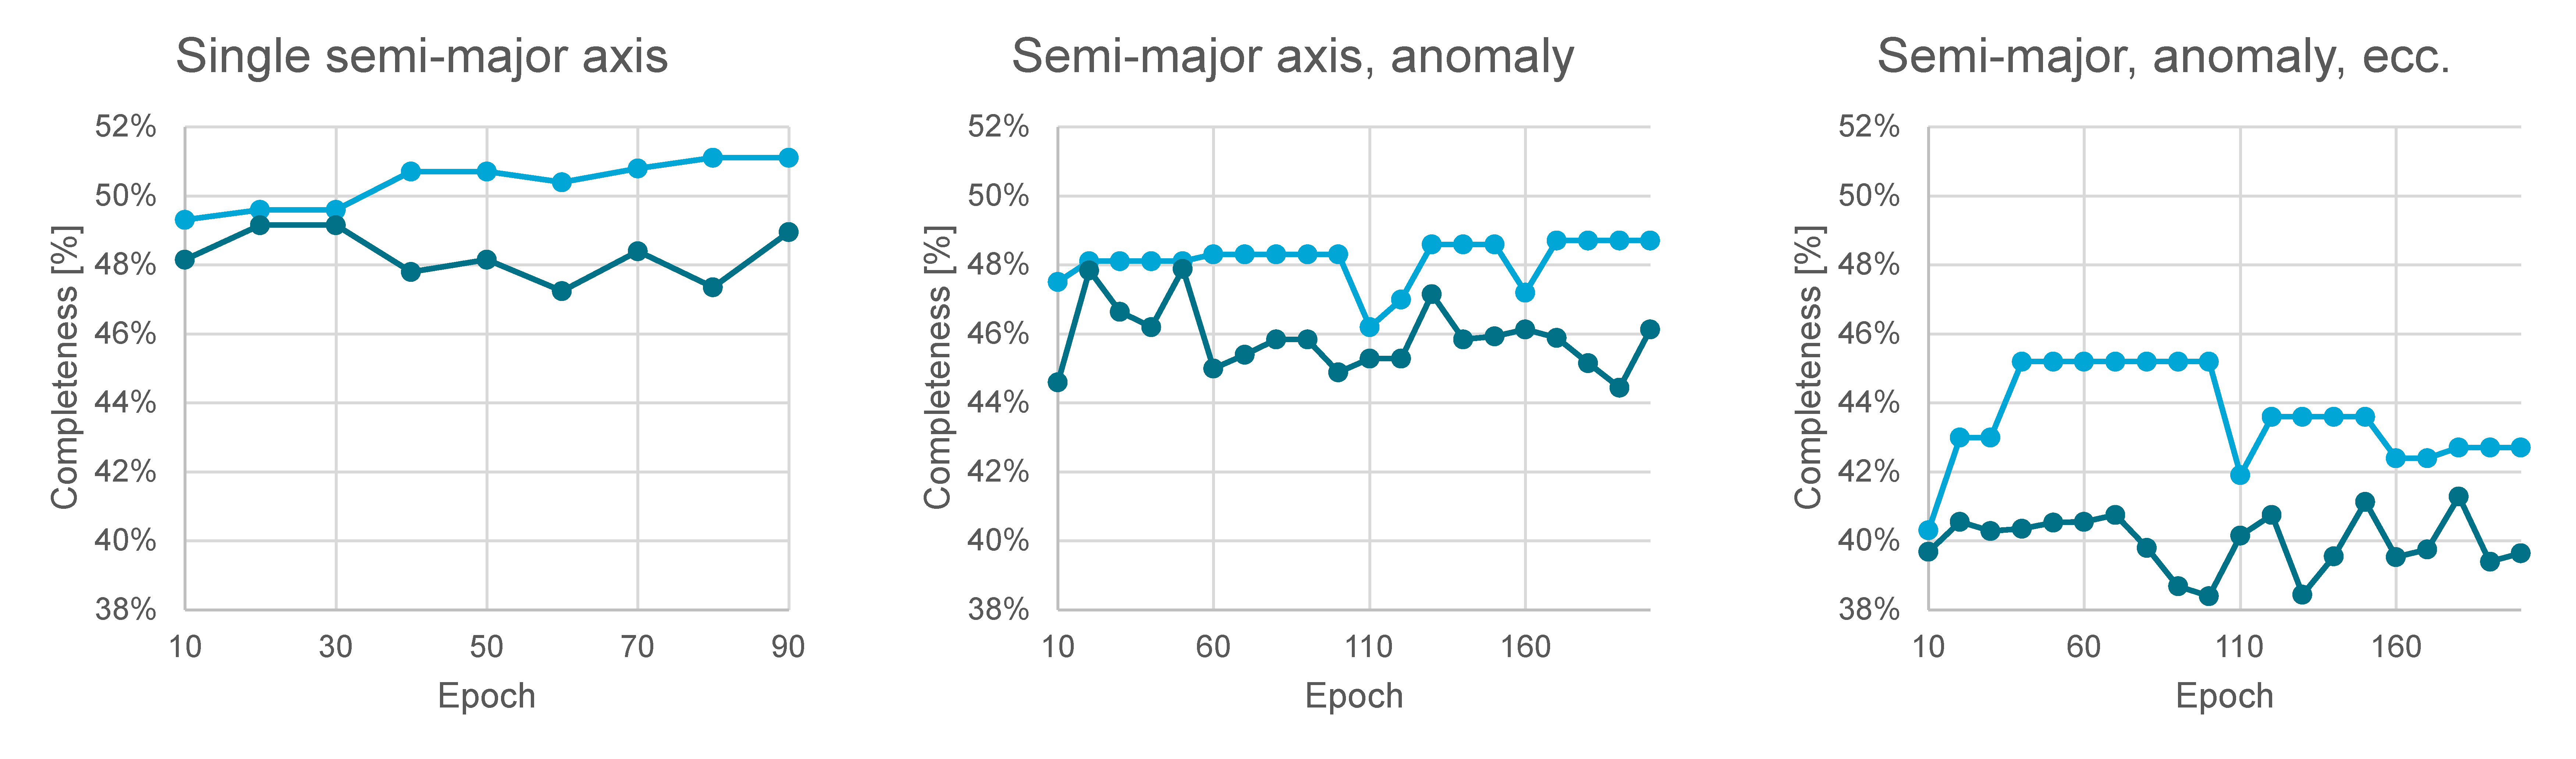
\includegraphics[width=1.0\textwidth]{img/val_orbits_11.pdf}
 \caption{Learning/validation results for systems with eleven spacecraft.}
 \label{fig:val_orbits_11}
\end{figure}

\begin{table}[htbp]
\centering
\caption{Optimization results for 11 spacecraft.}
\label{tab:opt_11}
\begin{tabulary}{1.0\textwidth}{L|LLL}
                             & $a$                                                                                    & $e$                                                                             & $\theta$                                                                         \\ \hline
circular, co-orbital         & 1.443,   1.443, 1.443, 1.443, 1.443, 1.443, 1.443, 1.443, 1.443, 1.443, 1.443        & 0.000, 0.000, 0.000, 0.000,   0.000, 0.000, 0.000, 0.000, 0.000, 0.000, 0.000 & 0.000, 0.571, 1.142, 1.714,   2.285, 2.856, 3.427, 3.998, 4.570, 5.141, 5.712 \\
circular, non-co-orbital     & 0.870,   0.822, 1.220, 1.020, 1.447, 0.480, 0.217, 1.124, 1.714, 1.278, 1.573        & 0.000, 0.000, 0.000, 0.000,   0.000, 0.000, 0.000, 0.000, 0.000, 0.000, 0.000 & 2.062, 4.858, 2.753, 2.168,   2.834, 2.050, 0.609, 5.915, 1.006, 2.057, 2.701 \\
non-circular, non-co-orbital & 1.054,   1.416, 2.065, 1.132, 0.216, 0.191, 0.729, 1.267, 1.100, 1.588, 1.189, 0.248 & 0.190, 0.313, 0.519, 0.683,   0.438, 0.047, 0.817, 0.754, 0.586, 0.084, 0.155 & 2.86, 1.921, 5.046, 4.659,   5.717, 0.094, 4.036, 7.140, 4.715, 6.327        
\end{tabulary}
\end{table}

The last case to be considered is the 11-spacecraft case. The corresponding results can be seen in \autoref{fig:orbits_11}, \autoref{fig:val_orbits_11} and \autoref{tab:opt_11}. The performance of the non-circular system has deteriorated even further: the optimizer loses performance through succesive optimization epochs. In addition the non-co-orbital circular case has also lost good performance. Instead of a well-structured system, the optimizer places the spacecraft in orbits spaced semi-uniformly, and spends significant of effort optimizing the anomaly at epoch. Of course, for a system with differing semi-major axis, the anomaly is a relatively unimportant parameter, and therefore the validation performance can be seen to decrease throughout the process.\\

Clearly, the optimizer is not ideal for obtaining the best solutions across larger dimensionalities. However, an important conclusion can still be drawn from this fact: For lower numbers of spacecraft, the initial performance of the optimizer is still adequate. However, the increase in freedom of placing the spacecraft does in no case yield a statistically significant increase in performance. Recall that the variance in the result when modelling the system is approximately 1-2\%. This then means that no increase in freedom of placing the spacecraft for the region where the optimizer is well-behaved ($n < 11$ for the circular, non-co-orbital case, or $n < 6$ for the non-circular, non-co-orbital case) results in a performance increase of more than 1-2\%. Else, the optimizer would be expected to find this solution at least part of the time. This phenomenon is not inherent to the functioning of the optimizer. It still manifested itself when using a uniform random sampling method, which is more independent of the function to be optimized. However, as mentioned previously, this result is unexpected: to proof that the optimizer functions fully correctly, would require obtaining the same solution for all cases, should the circular, co-orbital case be the best choice. Therefore it can be concluded that for these numbers of spacecraft, a solution in which each spacecraft has its own orbit is probably not statistically superior to a co-orbital solution as alluded to in the previous section, however, problems with the optimizer preclude reaching a definite conclusion on this part. \\

Note that this does not necessarily extrapolate to these solutions \textit{never} being useful. Perhaps research into more complex search strategies, as mentioned previously, could still provide interesting opportunities for such a setup. In addition, it might seem counterintuitive that such a system would not be able to perform better than a system with only a single semi-major axis. Therefore, in the next section, the driving factor behind the systems performance will be investigated.\\


\section{Predicted Performance and Implications for Missions Design}
\label{sec:results_performance}
The last sections treated the reasoning behind the observed performance and how to obtain it. However in addition, it is important to consider what that performance can be expected to be, and how this might affect the design of future NEA survey missions. Therefore, using the optimal solutions found in this chapter, modelling was done to predict what performance might be expected of such a survey. The predictions for performance can be seen in \autoref{fig:performance_prediction}. Here, the projected performance of a system of 1 - 6 spacecraft is shown relative to the current knowledge of the NEA population (per \cite{HarrisPopulation}) and the projected population due to current efforts (as per \cite{2017NEOSDT}). It should be noted that the ``PROJ''-curve relates to the expected completion, in case \textit{no new survey efforts are started}. Comparison of the 1 S/C system in this report, and in \cite{2017NEOSDT} is performed in \autoref{sec:vvperformance}. In addition, the performance relative to the projection is shown in \autoref{fig:performance_prediction_rel}. It can be seen that firstly, any deep space NEA survey will vastly increase the knowledge of the NEA population, increasing the completeness by around 15-20\% at all absolute magnitudes < 20. Additionally, a second spacecraft in the system will yield an additional increase roughly equal in magnitude. After two spacecraft, diminishing returns become a serious factor on the performance. As can be seen in \autoref{fig:performance_prediction_rel}, such systems will still exhibit a sizeable gain in completeness. However, this gain will be centered mostly around the smaller NEAs, i.e., the $21 < H < 24$-range. Note that this follows also from the theory mentioned in the \autoref{sec:results_explanation}: as the number of spacecraft increases, the observable volume for large NEAs barely increases; only an increase among the smaller NEAs is observed (see \autoref{fig:coverage_spread}).\\


\begin{figure}[htbp]
 \centering
 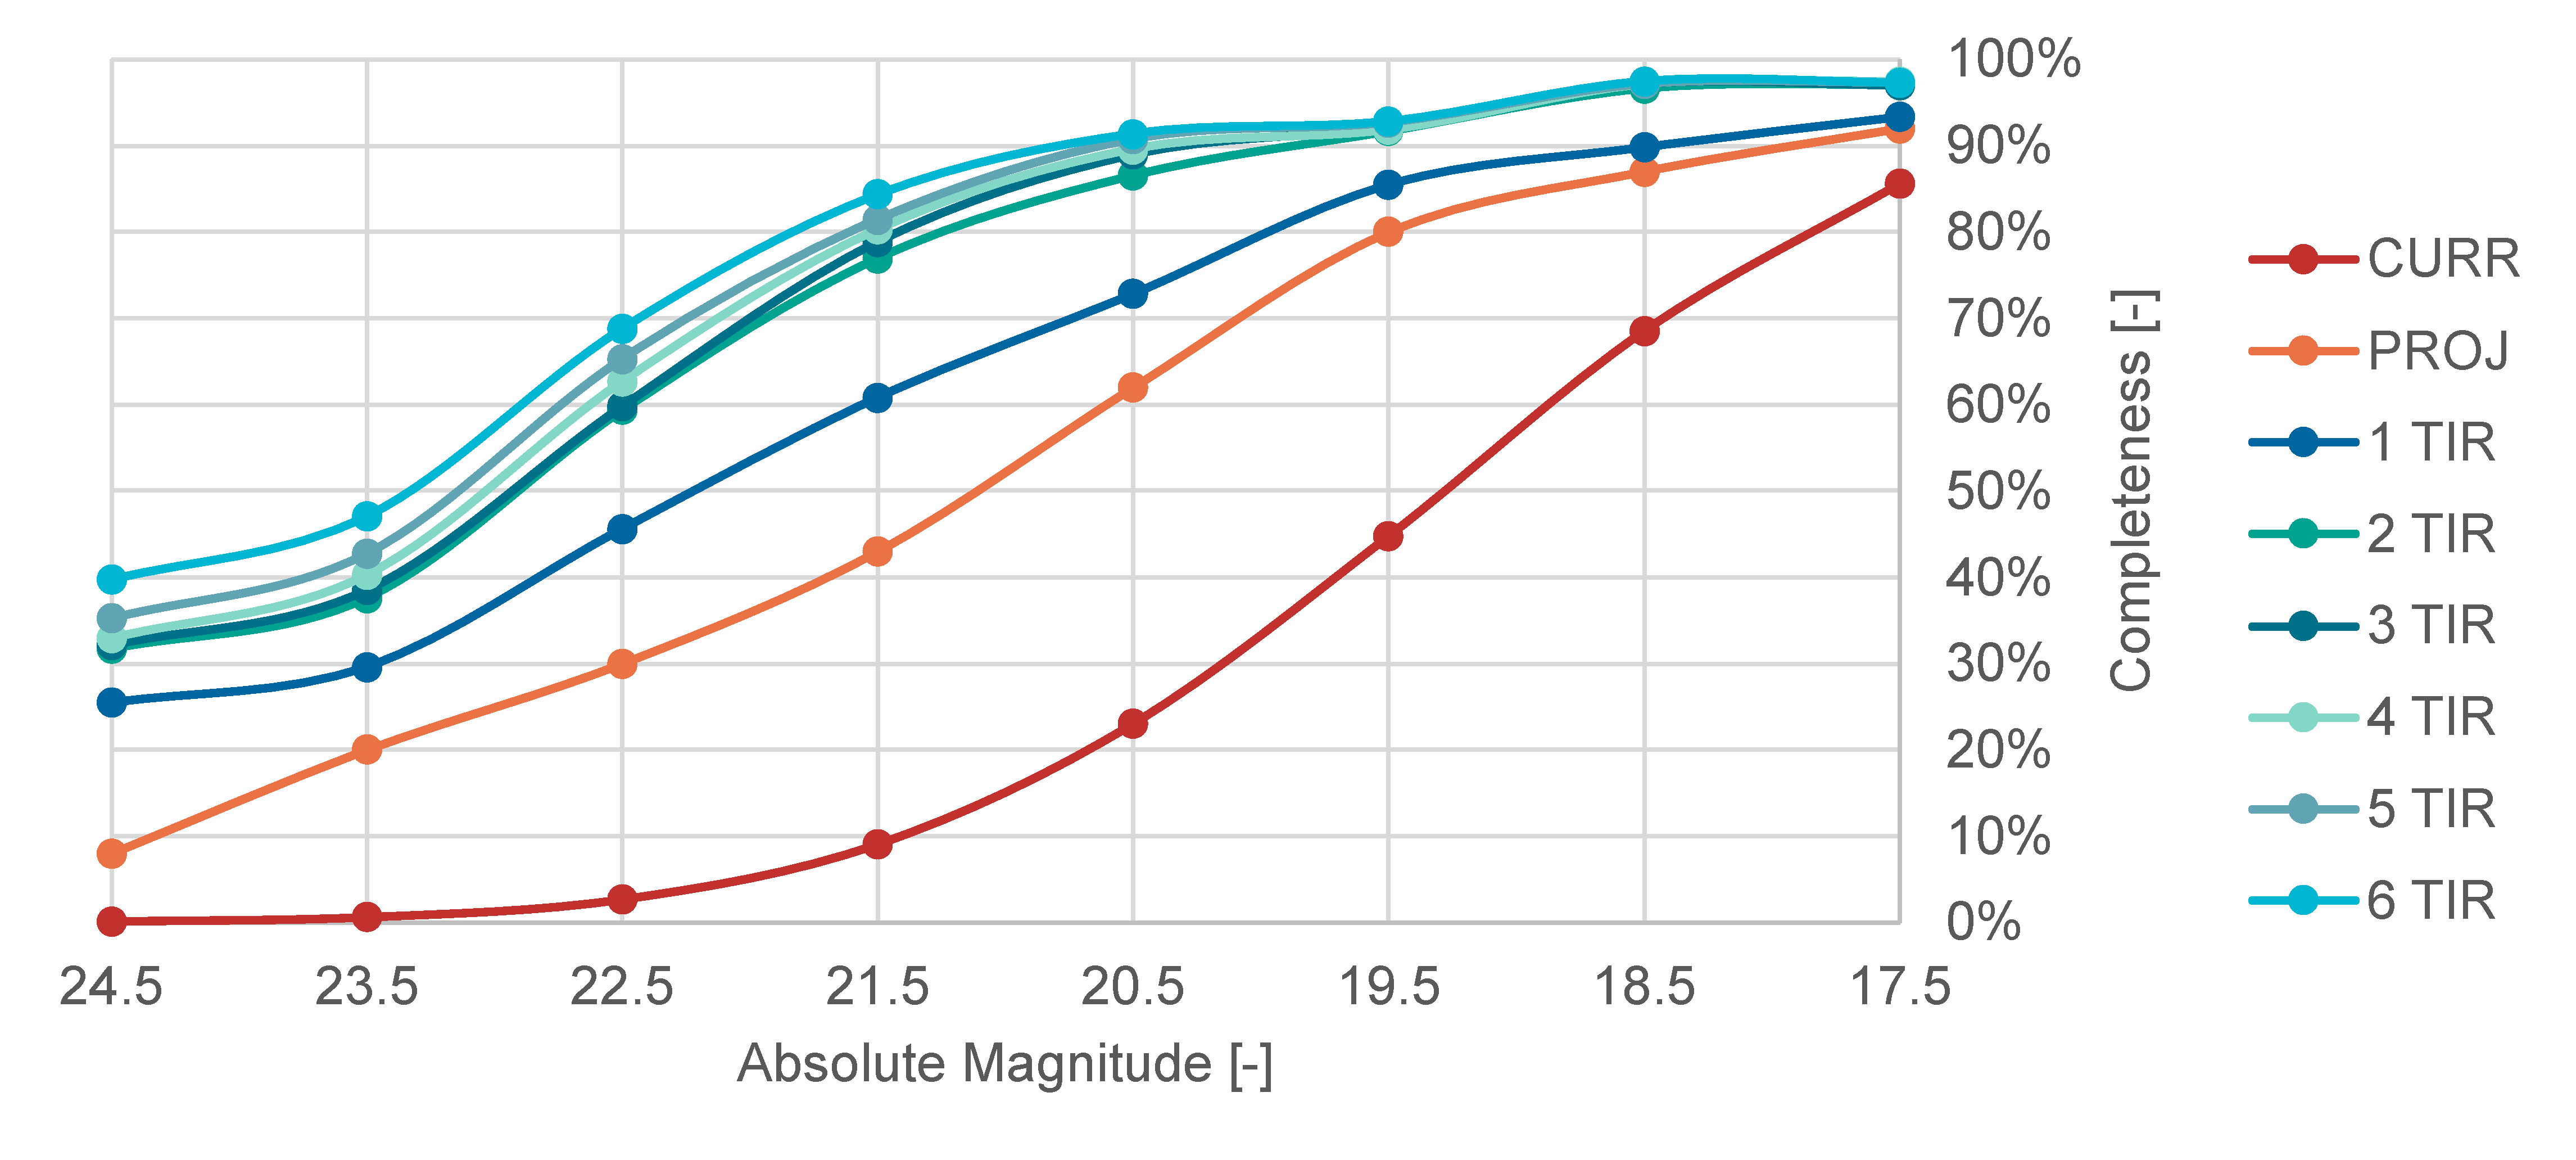
\includegraphics[width=0.9\textwidth]{img/performance_prediction.pdf}
 \caption{Prediction of performance}
 \label{fig:performance_prediction}
\end{figure}

\begin{figure}[htbp]
 \centering
 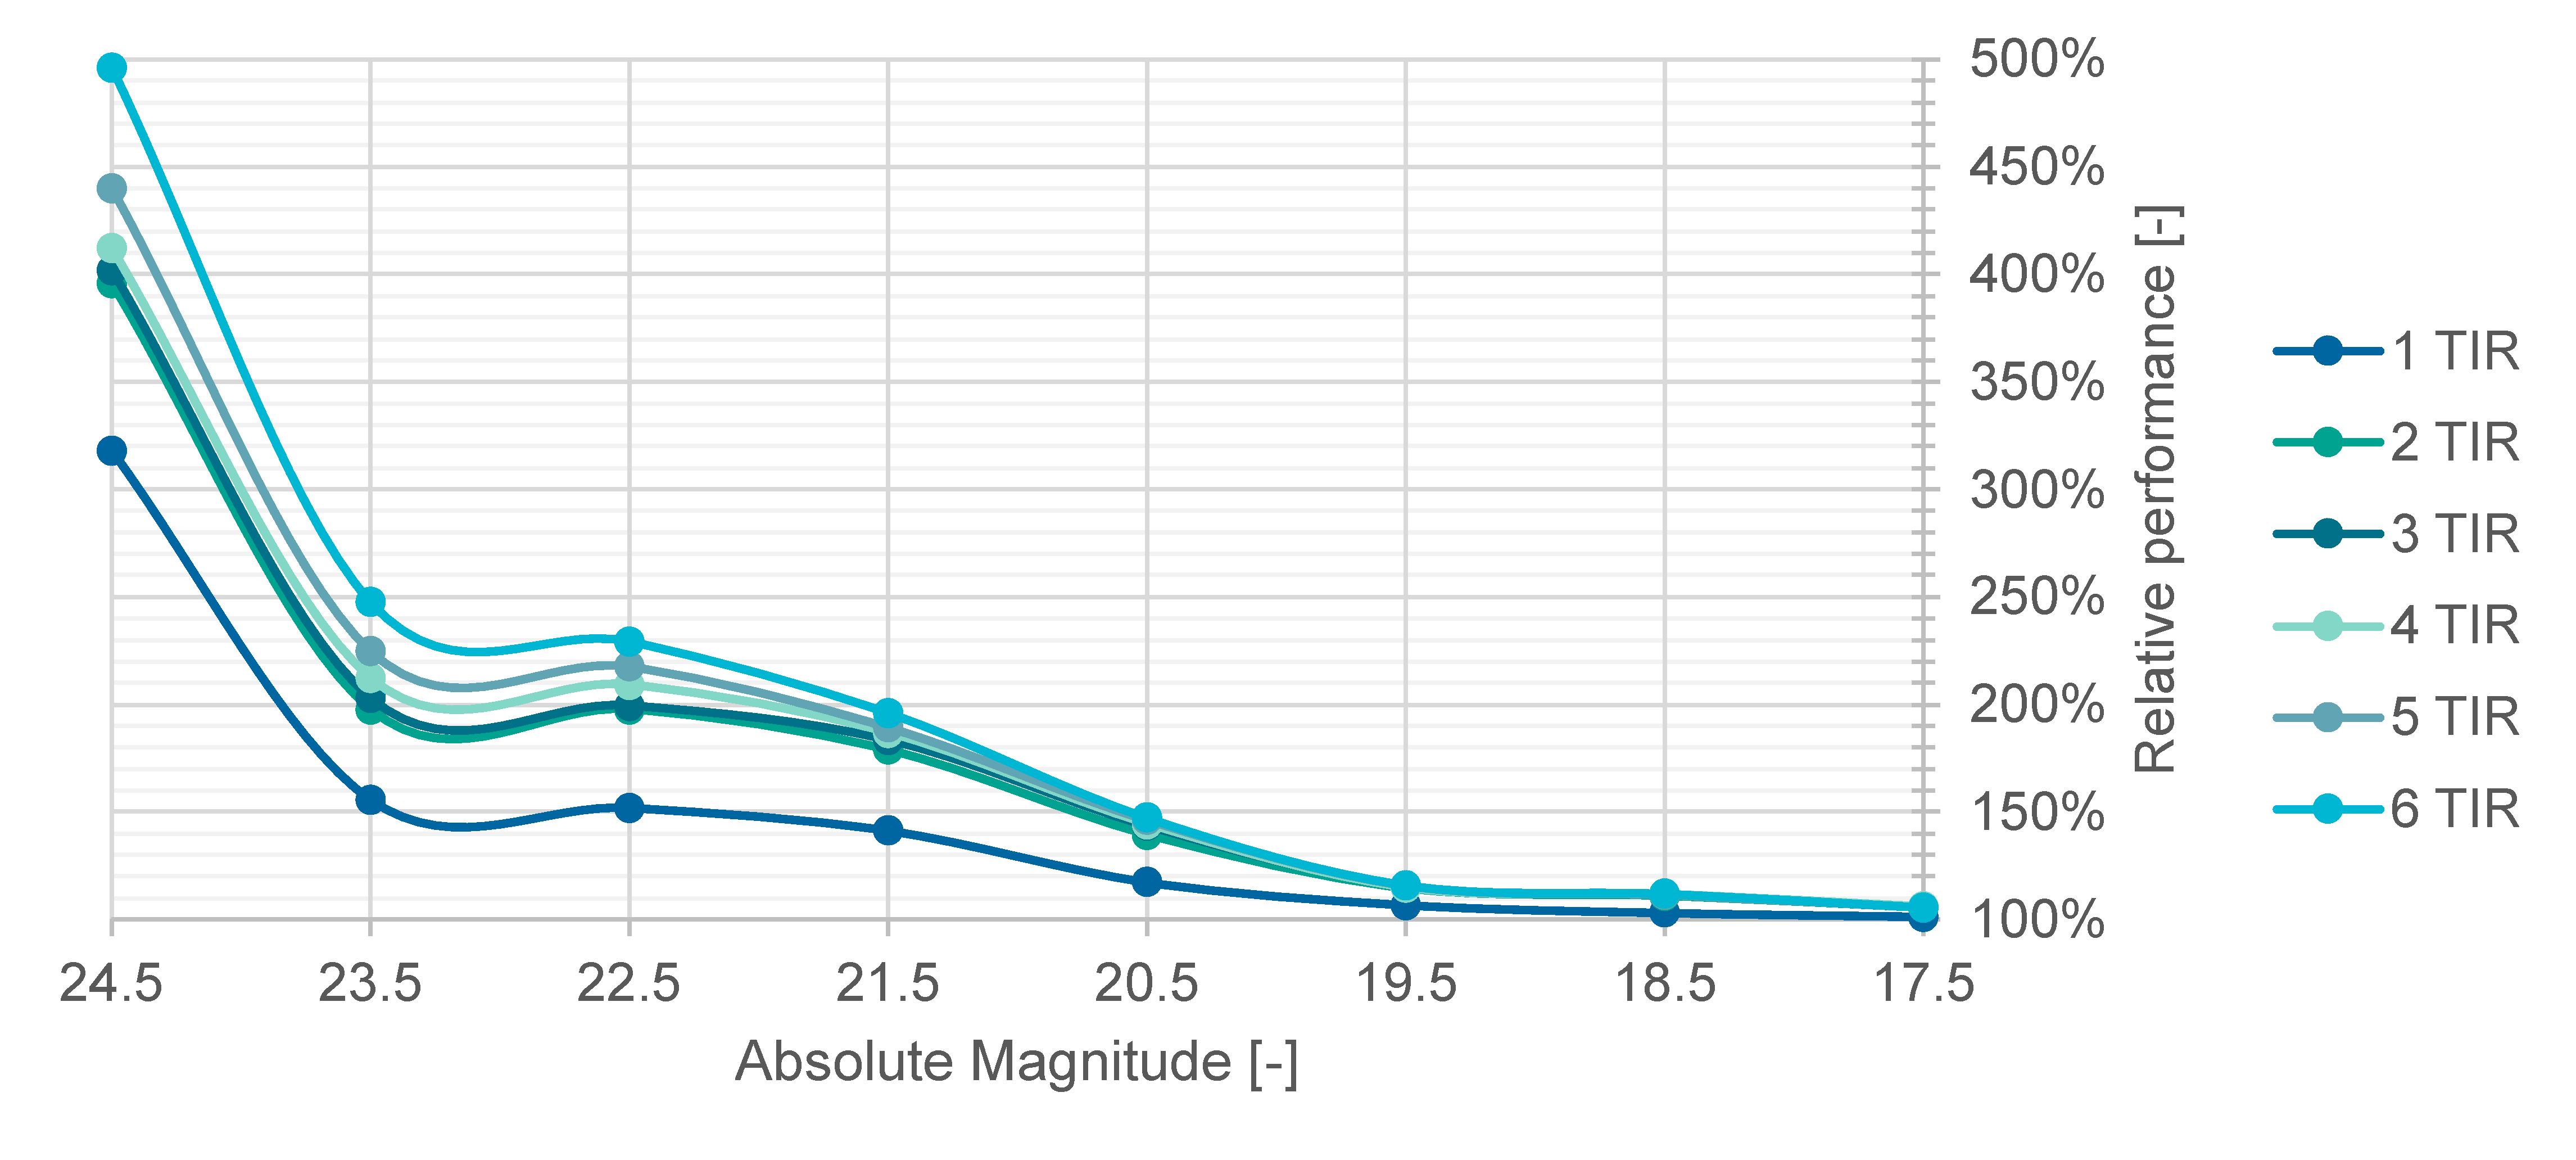
\includegraphics[width=0.9\textwidth]{img/performance_prediction_rel.pdf}
 \caption{Relative prediction of performance}
 \label{fig:performance_prediction_rel}
\end{figure}

Furthermore, a mission designer might be interested in what number of spacecraft would be required to reach a specific level of completeness across the NEA population. Reason for this is that, as seen in the past (e.g. \cite{2003NEOSDT}), objectives are often formulated in terms of a specific completeness level. For this reason, simulations were performed up to 200 spacecraft. The result of this was that the performance follows a roughly logarithmic progression, as can be seen in \autoref{fig:completeness_hypothetical}. Even for extremely large systems of more than 100 spacecraft, completeness nears only 70\%. This occurs as any synergistic benefits of a multi-spacecraft system, as explained in \autoref{sec:researchmultispacecraft} have been obtained at lower numbers of spacecraft already, and higher numbers of spacecraft only provide more frequent imaging capabilities. Therefore, this strong diminishing returns effect is observed. Obviously, such a large system will not be constructed in the near future, and therefore such a goal is seen as unfeasible considering current hardware and software capabilities. Numerically, the relevant values indicate that in order to reach 20\% completeness, 1 spacecraft suffices; for 30\%, a second spacecraft is sufficient. Then, to reach 40\% completeness requires a 6 spacecraft system. 50\% completeness is obtained at 15 spacecraft, 60\% at around 50 spacecraft and lastly, at 200 spacecraft, around 70\% completeness is achieveable. Although not simulated due to practical limitations, it is estimated that around 500 spacecraft would be required to reach 80\% completeness.

\begin{figure}[htbp]
 \centering
 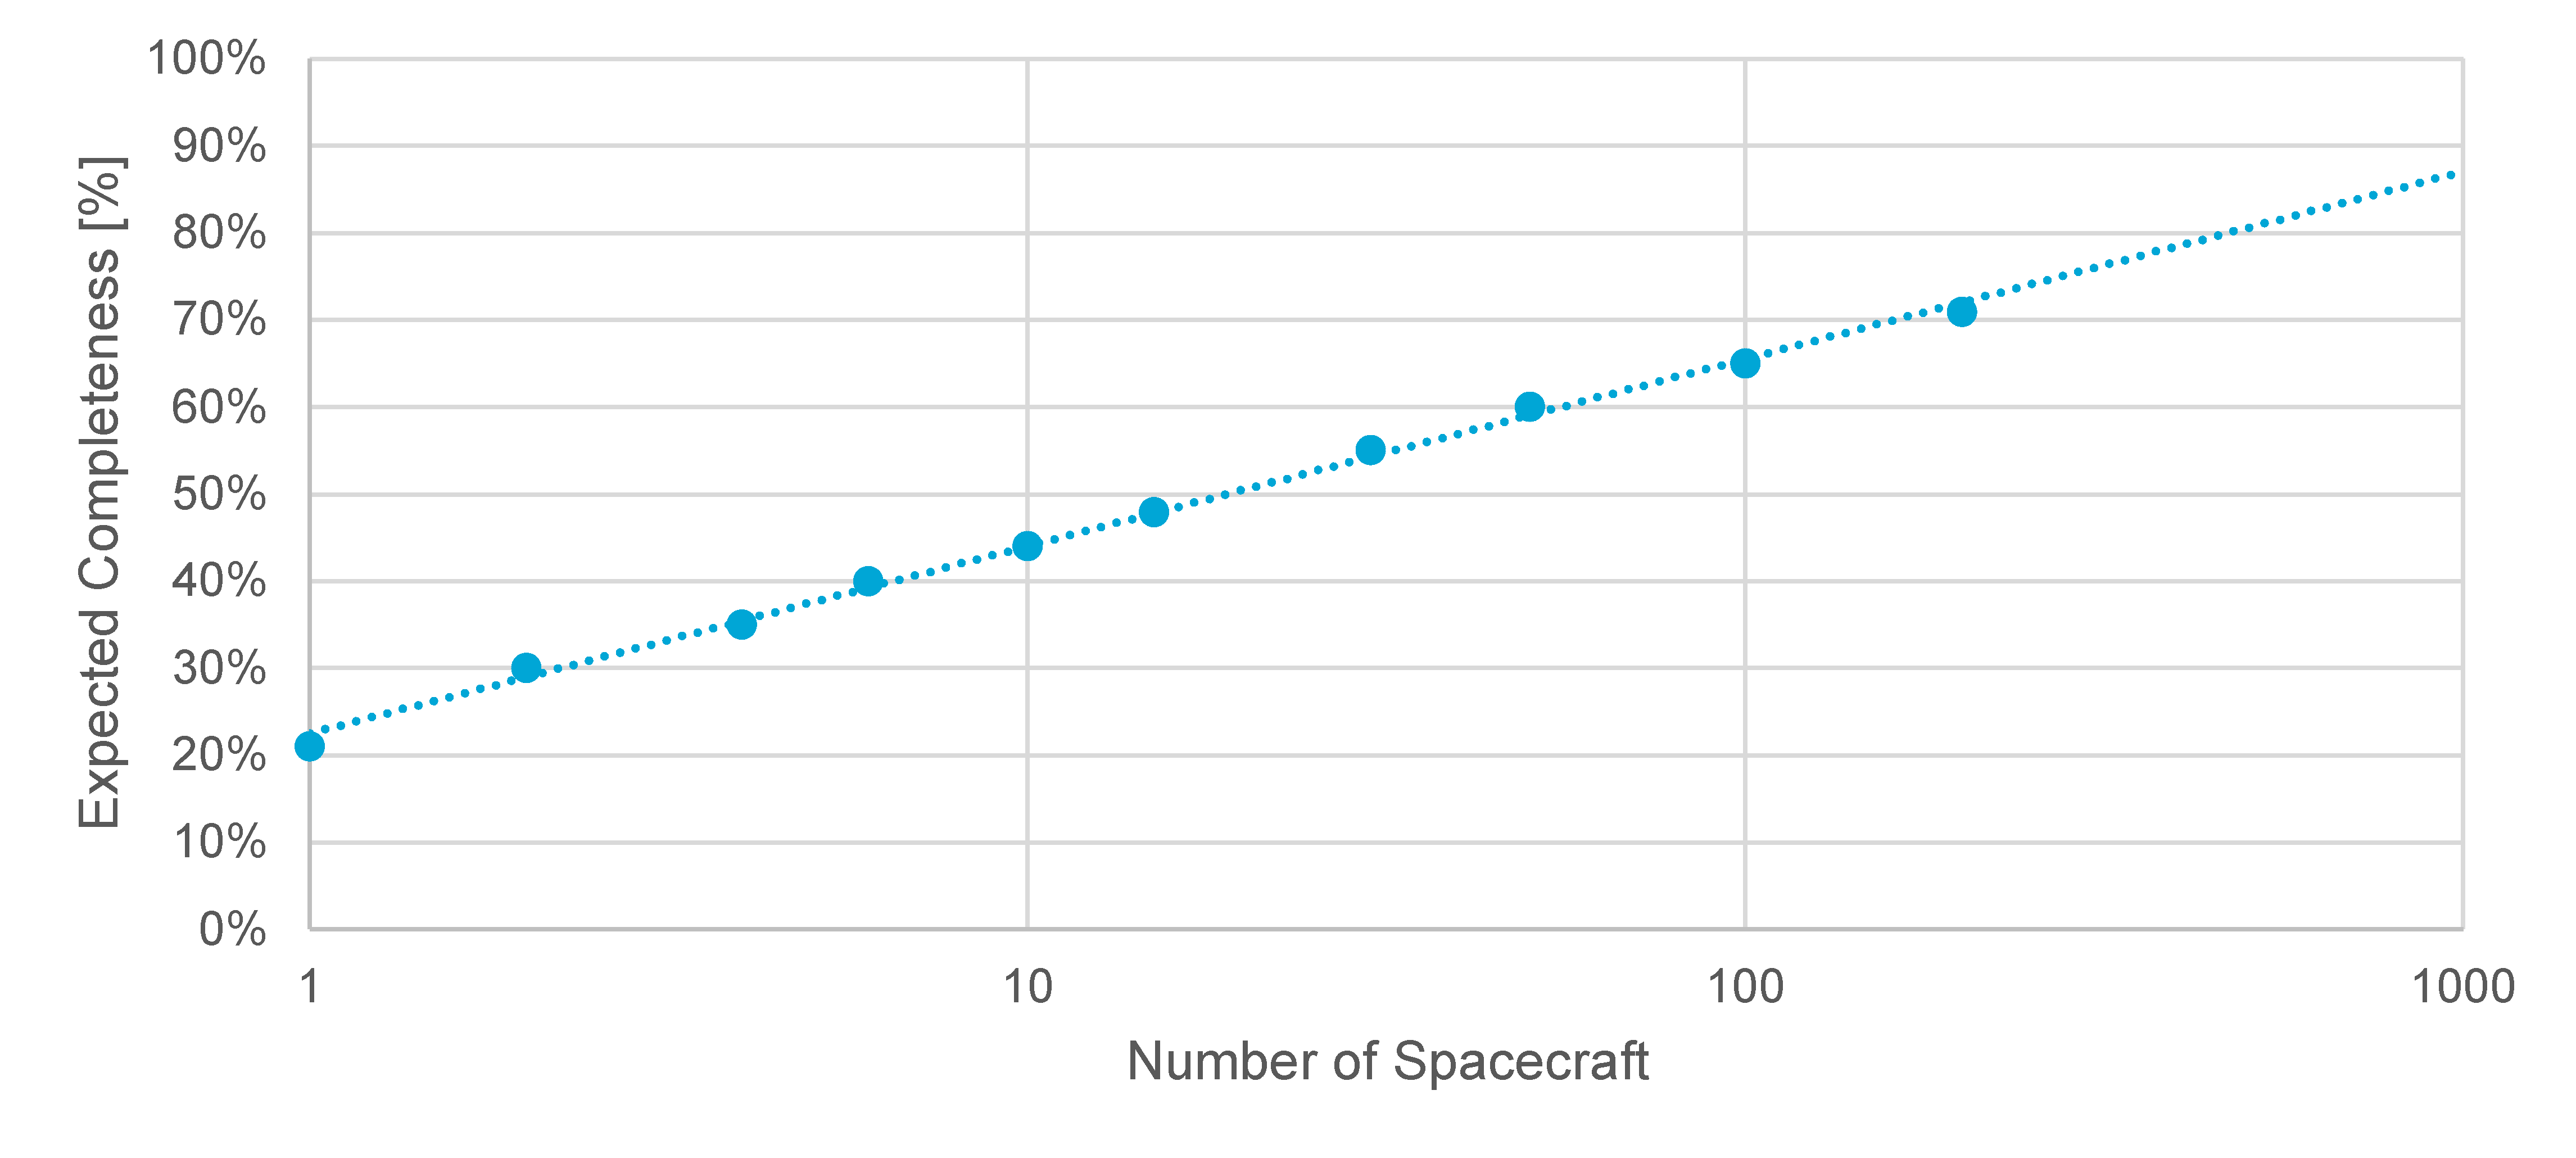
\includegraphics[width=0.8\textwidth]{img/completeness_hypothetical.pdf}
 \caption{Expected performance as a function of number of spacecraft.}
 \label{fig:completeness_hypothetical}
\end{figure}

In conclusion, using currently available search strategies and hardware, optimal solutions can be found by optimizing the system for a single semi-major axis, and spreading out the spacecraft equally throughout the orbit, as this maximizes the observable volume available to the system. The resulting increase of completeness from a single-spacecraft system is around 15-20\% across all NEA sizes smaller than $H=20$. Addition of a second spacecraft raises this performance by a large amount across all NEA sizes, and is defninitely worthy of consideration. Higher numbers of spacecraft only yield small increases in the lower NEA sizes as there is a strong presence of diminishing returns. Lastly, advances in hardware or software technology will be required to feasibly reach higher numbers of completeness in the future, should this be considered. In the next chapter, the accuracy of these results will be examined through the process of verification and validation.

\newpage
\chapter{Sensitivity Analysis}

\section{Expected Performance}

\section{Optimization Results}

\section{Hardware and Survey Properties}

\newpage
\chapter{Conclusion and Recommendations}
\label{ch:conclusion}
The aim of this report was to evaluate the possibilities and capabilities for surveying Near-Earth Asteroids using a system of multiple spacecraft. The main question to be answered was: ``What is the optimal position and composition for a system of spacecraft with the purpose of identifying and cataloguing previously unidentified Near-Earth Asteroids?''. To conclude the report, here the main question and associated subquestions will be answered, and conclusions will be drawn from these answers which can be used in the design of future NEA survey missions. In addition, during research several opportunities were found for further research to better understand the capabilities of multi-spacecraft NEA surveys and to further develop the technology required to realise them. These opportunities will be turned into recommendations for future research.

\section{Conclusions}
Before summarizing the conclusions of the report, concrete answers to the research questions drafted in \label{sec:researchquestions} will be provided. Firstly, the various subquestions can be adressed:

\begin{enumerate}
 \item \textbf{How can the population of NEAs be accurately modelled, and how can these models be adjusted for unidentified NEA's?}: Modelling the population of NEA's was performed using a model created with the aid of NEOWISE data, compensated for biases in observation. This model was published by \cite{GranvikPopulation}, and is publicly available. As research focussed on still unidentified NEA's, the population was corrected with completeness statistics calculated from NEOWISE data by \cite{HarrisPopulation}. 
 \item \textbf{How can surveys of NEA's by a system of spacecraft be accurately modelled?}: Surveys were modelled by explicit calculation of the important steps in the process. First, the positions of all asteroids and spacecraft are calculated according to Keplerian orbits. Then, the background signal and target signals are calculated. From this, using representative hardware parameters, the signal-to-noise ratio can be obtained. Lastly, a probabilistic detection model is used to establish detection, and integration of the system in time allows for establishing identification. Components of the system were found from various sources in peer-reviewed literature, and their implementation was thoroughly verified and validated. In addition, it was shown that the simulation yielded similar results as other, previously validated survey models.
 \item \textbf{How can the position and composition of the system be optimized?}: The main challenge involved in optimizing the system is the fact that no useful analytical properties, such as gradients, are available, and the fact that the survey model is computationally expensive. For this reason, an approach of surrogate optimization was implemented. It was shown that this optimization yielded results close to what was expected to be the optimum. However, when larger numbers of parameters were introduced into the optimization, overfitting reduced the accuracy of the results.
 \item \textbf{What is the effect of increasing the number of spacecraft on the process and performance of identifying and cataloguing NEA's?}: It was found that performance continuously increases with an increasing number of spacecraft. Initially, a second spacecraft yields very high improvements in performance - close to 50\% for thermal infrared systems - due to the possibility of performing triangulation, allowing for faster NEA identification. As the number of spacecraft further increases, the relative performance increase exponentially decreases. Therefore, systems with a large number of spacecraft will most likely not be cost-efficient compared to systems with less spacecraft, however addition of a second or third spacecraft will yield sizeable performance increases nonetheless.
 \item \textbf{How is the performance of possible payload compositions affected by the number of spacecraft, and what is the resulting optimal payload composition?}: It was shown that thermal infrared telescope payloads are the best choice for a future deep space NEA survey mission. Not only are thermal infrared telescopes superior to visual light telescopes for single spacecraft systems, the research presented in this report also shows that the relative performance increase of a thermal infrared system as the number of spacecraft is increased is higher than that of a visual light system. In addition, it was shown that for practical numbers of spacecraft, so-called ``hybrid'' systems with both visual light and thermal infrared telescopes did not provide enough synergistic benefits to outweight the worse performance of the visual light telescope.
 \item \textbf{How do the number of spacecraft and payload interact with the orbital parameters of the system?}: It was found that optimally, the spacecraft should be situated in a circular orbit, equally spaced out. The semi-major axis of said orbit increases as the number of spacecraft increases, because the spacecraft are placed closer together, introducing an inefficient overlap in their observation areas.
 \item \textbf{How effective is a system of multiple spacecraft at identifying and cataloguing previously unidentified NEA's compared to other current and future methods?}: A system of multiple spacecraft was shown to provide significant performance benefits to a single spacecraft system. Addition of a second spacecraft is expected to increase the improvement in completeness granted by a single spacecraft system by more than 50\% for asteroids in the tens to hundreds of meters in diameter. Further increases in the number of spacecraft will still yield improvements, however as the number of spacecraft increases, the majority of improvement will occur in the small, sub-100m diameter ranges.
\end{enumerate}

After answering the subquestions, the main research question can be adressed: ``What is the optimal position and composition for a system of spacecraft with the purpose of identifying and cataloguing previously unidentified Near-Earth Asteroids?'' Through the research, it was found that the optimal NEA survey using multiple spacecraft should utilize the following:
\begin{itemize}
 \item \textbf{Number of spacecraft}: The number of spacecraft is dependent on the desired performance. It was shown that increasing the number of spacecraft will continue to increase the performance of the system, even when the system contains tens to hundreds of spacecraft. However, diminishing returns quickly set it and economic considerations should be included if an optimum is to be found.
 \item \textbf{Orbit}: The optimal orbit for the system was found to be a circular orbit, with the spacecraft spread out over the full circle of the orbit. In this way, the total volume of space effectively covered by the spacecraft is maximized, and does not vary in time.
 \item \textbf{Orbital radius}: The semi-major axis of the orbit should increase with increasing number of spacecraft, to reduce the overlap in spacecraft observation coverage as the distance between spacecraft reduces. Initially, for a single spacecraft, the optimum is found around 0.8 AU. For 2 or 3 spacecraft systems, the optimum lies around 1.0 AU. For a 4 to 5 spacecraft system, the optimal radius increases to around 1.1 AU. Further spacecraft will yield further increase of the semi-major axis. It was also found that the semi-major axis is not a very sensitive parameter for the performance, and deviation of up to 0.1 AU from the optimum will result in no statistically significant degradation of performance.
 \item \textbf{Payload}: Lastly, the system should be composed of spacecraft using telescopes built for imaging in the thermal infrared spectrum. As already shown by previous research, thermal infrared is preferred over visual light systems, as the background signal is weaker, leading to better signal-to-noise ratios for small targets. In addition, this research has shown that the relative benefit of using multiple spacecraft is greater when using thermal infrared telescopes. In addition, it is expected that thermal infrared sensor technology will still improve substantially in the coming years, adressing current shortcomings such as small sensor field-of-views and long integration times. This will improve the performance even further.
\end{itemize}

In conclusion, an analysis was provided of the behavior, ideal parameters, and expected performance of a multi-spacecraft NEA survey. Through answering the research question, a set of guidelines was obtained which can be used either directly in a design effort towards further surveying missions, or as a basis for future research. To facilitate in carrying out this research, the next section will provide some recommendations with regards to possible avenues to explore next.

\section{Recommendations for Further Research}
Throughout the research, several opportunities were identified to improve the understanding of multi-spacecraft NEA systems, or to further develop the necessary technologies. These form the basis of the recommendations listed below:
\begin{itemize}
 \item \textbf{NEA survey search strategies}: Currently, very little literature exists on the strategy that should be used for searching for NEA's. Although algorithms exists for single-spacecraft surveys, they are not extensively researched. In addition, no work has been done to exploit the possibilities of multi-spacecraft search strategies. For example, telescopes could focus their search effort in an area where another telescope has detected an NEA, or search strategies could be set up to maximize the occurence of triangulation, speeding up detection efforts significantly and helping to detect small, fast travelling NEA's.
 \item \textbf{On-board processing and communication limitations}: Throughout this report, it was assumed that spacecraft are capable of processing images from the telescopes and communicating within the system and to Earth. However, neither of these capabilities are currently proven (see \cite{LiteratureReview} for a full exploration). Therefore, work should be done on how a multi-spacecraft system can efficiently process and communicate the survey data.
 \item \textbf{Adressing the overfitting of the optimizer}: Detailed optimization efforts were hindered by a growing amount of overfit manifesting in the optimization efforts. As this thesis is not focussed on the topic of machine learning, and sufficient conclusions could be drawn, these results were left at that. However, to confirm the expectation that no significantly better solutions exists, it is suggested to attempt an optimization method which is less susceptible to noise in the signal. The recommendation would be to first attempt a different surrogate model, such as using an artificial neural network, instead of a classical machine learning approach, and possibly branching our further from that.
 \item \textbf{Investigation of the problem in non-Keplerian celestial mechanics}: Although the error in the solution is expected to be small, it is recommended to validate this by performing a three-body or n-body simulation of the problem. This might also interplay with advances in the search strategies, as more subtleties in the orbits of NEA's become important for the performance. In addition, non-Keplerian mechanics might allow exploitation of different orbital configurations for the system of spacecraft. In particular, utilization of Lagrange point could allow for implementation of differing semi-major axes per spacecraft, whilst still maintaining a constant distance between the spacecraft throughout their mission.
\end{itemize}

\newpage

%% Use letters for the chapter numbers of the appendices.
\appendix

\printbibliography

\chapter{Verification and Validation}

\section{Modelling of Observations}

\section{Survey-specific Properties}

\section{Survey Performance}

\section{Optimization}




\end{document}

